%%%%%%%%%%%%%%%%%%%%%%%%%%%%%%%%%%%%%%%%%%%%%%%%%%%%%%%%%%%%%%%%%%%%%%%%%%%%
% AGUJournalTemplate.tex: this template file is for articles formatted with LaTeX
%
% This file includes commands and instructions
% given in the order necessary to produce a final output that will
% satisfy AGU requirements, including customized APA reference formatting.
%
% You may copy this file and give it your
% article name, and enter your text.
%
% guidelines and troubleshooting are here: 

%% To submit your paper:
\documentclass[draft]{agujournal2019}
\usepackage{url} %this package should fix any errors with URLs in refs.
\usepackage{lineno}
\usepackage[inline]{trackchanges} %for better track changes. finalnew option will compile document with changes incorporated.
\usepackage{soul}
\linenumbers
%%%%%%%
% As of 2018 we recommend use of the TrackChanges package to mark revisions.
% The trackchanges package adds five new LaTeX commands:
%
%  \note[editor]{The note}
%  \annote[editor]{Text to annotate}{The note}
%  \add[editor]{Text to add}
%  \remove[editor]{Text to remove}
%  \change[editor]{Text to remove}{Text to add}
%
% complete documentation is here: http://trackchanges.sourceforge.net/
%%%%%%%

\draftfalse

%% Enter journal name below.
\journalname{JGR: Space Physics}


\begin{document}

%%%%%%%%%%%%%%%%%%%%%%%%%%%%%%%%%%%%%%%%%%%%%%%
%  TITLE
%
% (A title should be specific, informative, and brief. Use
% abbreviations only if they are defined in the abstract. Titles that
% start with general keywords then specific terms are optimized in
% searches)
%
%%%%%%%%%%%%%%%%%%%%%%%%%%%%%%%%%%%%%%%%%%%%%%%

% Example: \title{This is a test title}

\title{Propagation of Interplanetary Shocks in the Heliosphere}

%%%%%%%%%%%%%%%%%%%%%%%%%%%%%%%%%%%%%%%%%%%%%%%
%
%  AUTHORS AND AFFILIATIONS
%
%%%%%%%%%%%%%%%%%%%%%%%%%%%%%%%%%%%%%%%%%%%%%%%

\authors{M.~Lkhagvadorj\affil{1,2}, G.~Facsk{\'o}\affil{1,3,4,5}, A.~Opitz\affil{1}, P.~Kov{\'a}cs\affil{1}, D.~G.~Sibeck\affil{4}}

\affiliation{1}{Department of Space Physics and Space Technology, Wigner Research Centre for Physics}
\affiliation{2}{Faculty of Science, Eötvös Loránd University}
\affiliation{3}{Department of Informatics, Milton Friedman University}
\affiliation{4}{NASA Goddard Space Flight Center}
\affiliation{5}{the Catholic University of America}

\affiliation{1}{Konkoly-Thege Mikl{\'o}s {\'u}t 29-33., H$-$1121~Budapest, Hungary}
\affiliation{2}{P{\'a}zm{\'a}ny P{\'e}ter s{\'e}t{\'a}ny 1/A, H$-$1117~Budapest, Hungary}
\affiliation{3}{H-1039 Budapest, Kelta utca 2., Budapest, Hungary}
\affiliation{4}{8800 Greenbelt Rd, Greenbelt, MD 20771, USA}
\affiliation{5}{620 Michigan Ave NE, Washington, DC 20064, USA}

\correspondingauthor{G{\'a}bor Facsk{\'o}}{facsko.gabor@wigner.hu}



%%%%%%%%%%%%%%%%%%%%%%%%%%%%%%%%%%%%%%%%%%%%%%%
% KEY POINTS
%%%%%%%%%%%%%%%%%%%%%%%%%%%%%%%%%%%%%%%%%%%%%%%
%  List up to three key points (at least one is required)
%  Key Points summarize the main points and conclusions of the article
%  Each must be 140 characters or fewer with no special characters or punctuation and must be complete sentences

\begin{keypoints}
\item Wave dispersion of IP shocks cannot be observed in the range of 40\,million\,km.
\item The shape of two IP shocks is determined from conjugated spacecraft observations.
\item These IP shocks are developed from coronal interaction regions.
\end{keypoints}

\begin{abstract}
 Interplanetary shocks are one of the crucial dynamic processes in the Heliosphere. They accelerate particles into a high energy, generate plasma waves, and could potentially trigger geomagnetic storms in the terrestrial magnetosphere disturbing significantly our technological infrastructures. In this study, two IP shock events are selected to study the temporal variations of the shock parameters using magnetometer and ion plasma measurements of the STEREO$-$A and B, the Wind, Cluster fleet, and the ACE spacecraft. The shock normal vectors are determined using the minimum variance analysis (MVA) and the magnetic coplanarity methods (CP). During the May 7 event, the shock parameters and the shock normal direction are consistent. The shock surface appears to be tilted almost the same degree as the Parker spiral, and the driver could be a CIR. During the April 23 event, the shock parameters do not change significantly except for the shock $\theta_{Bn}$ angle, however, the shape of the IP shock appears to be twisted along the transverse direction to the Sun-Earth line as well. The driver of this rippled shock is SIRs/CIRs as well. Being a fast-reverse shock caused this irregularity in shape.
\end{abstract}


\section*{Plain Language Summary}
The Sun dominates the Solar System gravitationally, magnetically, and by a very fast magnetized flow, called solar wind. In this matter strong and steep waves are moving, so-called interplanetary (IP) shocks. The parameters of the solar wind, the density, the magnetic field, the solar wind speed, and the temperature jump when you pass these waves. These IP shocks are usually measured by a single spacecraft. Therefore, their shape is supposed to be a plane. Using various multiple probes we determine the shape of two IP shocks. Additionally, we check whether the parameters of shocks change temporarily. If you throw a stone into a lake circular waves are triggered on the surface of the water. During their propagation, the width of the wave increases because the waves are a branch of waves, the so-called wave package. The wave package consists of waves propagating at different speeds. This feature is called wave dispersion. You cannot see any sign of wave dispersion or temporal development of the IP shock in the range of 40\,million\,km. 


\section{Introduction}
\label{sec:intro}

The solar corona is hotter than the photosphere, the chromosphere, and the transient layers beneath it. As a result, the high temperatures ionize atoms, creating a plasma of free-moving electrons and ions, the so-called the solar wind. Historically, \cite{parker58:_dynam_inter_gas_magnet_field} predicted the existence of the solar wind and made the term. He deducted it based on German astronomer Ludwig Bierman's observation of how the comet tail always points away from the Sun \cite{biermann57:_solar}. The existence of the solar wind was confirmed by the Mariner 2 spacecraft \cite{snyder65:_inter_solar_wind_measur_marin_ii}. The solar wind is a collisionless plasma, and it flows at both supersonic and super-Alfvénic speed, meaning they exceed the Alfv{\'e}n speed, which is the speed of magnetohydrodynamic waves in a plasma. A shock wave is where a fluid changes from supersonic to subsonic speed. Therefore, the fast-moving solar wind tends to create a shock on its journey. Hence, interplanetary (IP) shocks are common through the heliosphere, which is a bubble-like region of space surrounding the Sun and extending far beyond the orbits of the planets and is filled with the solar wind. There are a few varieties of shocks such as planetary bow shocks, shocks that are risen due to the stream interaction regions (SIR), which is called co-rotation interaction region (CIR) when extending beyond 1 AU, and coronal mass ejection (CME) driven shocks. IP shocks are one of the main and efficient accelerators of energetic particles \cite{tsurutani85:_accel_au, keith21:_histor}. These accelerated particles can cause disturbances to the geomagnetic field and are hazardous to astronauts and satellites. (IP) shocks driven by CMEs triggers large geomagnetic storms \cite{gonzalez94:_what}. Large geomagnetic storms can damage oil and gas pipelines and interfere with electrical power infrastructures. GPS navigation and high-frequency radio communications are also affected by ionosphere changes brought on by geomagnetic storms \cite{cid14} and can cause internet disruptions around the world for many months \cite{jyothi21:_solar_super}. Therefore, IP shocks are important in determining and understanding space weather.

The main goal of this paper is to study and determine parameters such as IP shock normals, upstream and downstream plasma parameters (magnetic field, density, temperature, velocity), and how they vary in their temporal evolution. There are several methods for determining the shock normal vector \cite{schwartz98:_shock_discon_normal_mach_number_relat_param}. Here, the minimum variance analysis (MVA) and the magnetic coplanarity method (CP) are used. These two methods are primarily utilized because they require solely magnetic field data. The data are from NASA Solar Terrestrial Relations Observatory \cite<STEREO;>{kaiser08:_stereo_mission}, the Wind \cite{ogilvie95:_swe_compr_plasm_instr_wind_spacec}, and  Advanced Composition Explorer \cite<ACE;>{stone98:_advan_compos_explor}, and ESA Cluster fleet \cite{escoubet01:_introd}. The temporal resolution of the magnetometers of the spacecraft is significantly higher than the plasma instruments because the variations are quite slow in the heliosphere. Hence, any agreement between the two methods indicates relatively accurate shock normal vectors \cite{facsko08:_clust,facsko09:_clust,facsko10:_study_clust}.

Here, two events are studied, one is on May 7, 2007, and the other is on April 23, 2007. The year 2007, is special because it was the year when the twin STEREO$-$A and B spacecraft were closer to the Sun-Earth line until their gradual separation from each other in the following years. Later, the spatial separation is so high that it is hard to distinguish the spatial and temporal changes. Hence, shocks during this period are proper to study shock propagation and their temporal developments in the case of using these spacecraft.

 %Chapter 4 is about instrumentation, database, and methods. Chapter 5 presents the results and discusses them. Chapter 6 is the summary and conclusions. 

\section{Missions and instruments}
\label{sec:mis}

In this paper, STEREO A and B, Wind, ACE, and the Cluster spacecraft magnetic field, ion plasma, and spacecraft potential data are used. 

\subsection{The STEREO mission}
\label{sec:stereo}

The twin STEREO A and B spacecraft were launched on October 26, 2006, from Kennedy Space Center \cite{kaiser08:_stereo_mission}. In heliospheric orbit at 1 AU, STEREO$-$A (Ahead) leads while STEREO$-$B (Behind) trails Earth. The two spacecraft separate at $44^{\circ}$ from each other annually. Both spacecraft were equipped with the complement of four scientific instruments, particularly two instruments and two instrument suites, with a total of 13 instruments on each spacecraft.

The PLAsma and SupraThermal Ion Composition (PLASTIC) instrument measures proton, the composition of heavy ions, and alpha particles in the solar wind plasma \cite{galvin08:_plasm_suprat_ion_compos_plast}. The In-situ Measurements of Particles and CME Transients magnetic field experiment (IMPACT) suite of instruments consists of seven instruments, and three of them are located on the 6-meter boom as shown while the others are in the main hull of the spacecraft \cite{acuna08:_stereo_impac_magnet_field_exper}. The IMPACT measures protons, heavy ions, and electrons, and the MAG magnetometer sensor in it measure the in situ magnetic fields in a range of $\pm 512\,nT$ with 0.1\,nT accuracy \cite{kaiser07:_stereo}. 

We downloaded all data from NASA's Coordinated Data Analysis Web (CDAWeb, \url{https://cdaweb.gsfc.nasa.gov/}). We obtained the STEREO$-$A and B magnetic field observation and the ion plasma data from the STEREO IMPACT with the time resolution of 100 ms and the STEREO PLASTIC instruuments, respectively. The magnetic field and the plasma data of the STEREO$-$A and B are in the RTN spacecraft coordinate system, where R is radially outward from the Sun, T is along the planetary orbital, and N is northward direction.

\subsection{The Wind mission}
\label{sec:wind}

NASA's Wind spacecraft was launched on November 1, 1994, \cite{wilson21:_quart_centur_wind_spacec_discov}. The Wind was initially planned sent to $L_1$ Lagrange point, however, was delayed to study the magnetosphere and lunar environment. Following a sequence of orbital adjustments, the Wind spacecraft was positioned in a Lissajous orbit close to the $L_1$ Lagrange point in early 2004 for studying the incoming solar wind \cite{team20:_wind_spacec}.

The spacecraft is equipped with the eight instruments, however, we used only the Magnetic Field Investigation \cite<MFI;>{lepping95:_wind_magnet_field_inves} and the Solar Wind Experiment \cite<SWE;>{ogilvie95:_swe_compr_plasm_instr_wind_spacec} measurements in this study. The MFI consists of two magnetometers at the 12-meter boom, its measurement capability is 4$\,$nT, 65536$\,$nT, and measures vector magnetic field up in a time resolution of 22 or 11 vectors per second for the calibrated high-resolution data and primary science data is in time resolutions of three seconds, one minute and one hour \cite{team22:_wind_data_sourc}. The SWE measures the solar wind key parameters such as velocity, density, and temperature. 

From CDAWeb, we got Wind magnetic and plasma data from the MFI instrument with a time resolution of 3\,s and SWE instrument with a time resolution of 1\,min, respectively. The magnetic field and the plasma data of the Wind are in the Geocentric Solar Ecliptic System (GSE) coordinate system, where X-axis is pointing to the Sun from the Earth, Y-axis is in the ecliptic plane against the planetary motion, and Z-axis is northward direction.

\subsection{The ACE mission}
\label{sec:ace}

NASA's ACE spacecraft was launched on August 25, 1997, \cite{stone98:_advan_compos_explor}. The spacecraft is located at $L_1$ Lagrangian point as well as the Wind spacecraft. The spacecraft is equipped with nine primary scientific instruments and one engineering instrument. We used in the study the measurements of the Magnetometer \cite<MAG;>{smith98:_ace_magnet_field_exper}, and  the Solar Wind Electron, Proton and Alpha Monitor \cite<SWEPAM;>{mccomas98:_solar_wind_elect_proton_alpha}. The MAG consists of twin triaxial flux-gate magnetometers such that magnetometer sensors have between 3 and 6 vectors $s^{-1}$ resolutions for continuous observation of the interplanetary magnetic field \cite{smith98:_ace_magnet_field_exper}. 

From CDAWeb, we downloaded the ACE magnetic and plasma data from the ACE MAG with a time resolution of 1\,s SWEPAM with the time resolution of 64\,s, respectively. The magnetic field and the plasma data are in both the RTN and GSE coordinate systems.

\subsection{The Cluster fleet}
\label{sec:cluster}

ESA's Cluster constellations consist of four satellites, which were launched on 16 July and 9 August 2000 \cite{escoubet01:_introd}. The Cluster satellites orbit in a tetrahedral formation around Earth. The orbits feature perigees close to four Earth radii ($R_E$) and apogees approximately 19.6\,$R_E$ away \cite{zhang10:_emic_he}. The four satellites are each equipped with 11 instruments. We used the data of the Cluster Ion Composition \cite<CIS;>{reme97:_clust_ion_spect_exper}, the Fluxgate Magnetometer \cite<FGM;>{balogh97:_clust_magnet_field_inves},  and the Electric field and waves \cite<EFW;>{gustafsson97:_elect_field_wave_exper_clust_mission} instruments in this study .

The FGM is composed of two tri-axial fluxgate magnetometers, which are installed on one of the two 5-meter radial booms. It measures in the dynamic range $\pm 65,536$\,nT. At the highest dynamic level, the resolution is  $\pm8$\,nT, and the time resolution is 100 vectors per second \cite{balogh97:_clust_magnet_field_inves,organization21:_fluxg_magnet_fgm}. The CIS instrument measures three-dimensional ion distribution, and it is composed of two distinct sensors: the Composition Distribution Function (CODIF) sensor and the Hot Ion Analyzer (HIA) sensor \cite{reme97:_clust_ion_spect_exper}. The CIS experiment is not operational for Cluster-2 and the HIA sensor is switched off for Cluster-4 due to a problem with the high voltage of the electrostatic analyzer \cite{team21:_clust_activ_archiv}. Hence, for Cluster-2 and Cluster-4, the EFW instrument measurement is useful \cite{gustafsson97:_elect_field_wave_exper_clust_mission}.

As the spacecraft travels through the plasma environment, it acquires an electric charge as a result of contact with charged particles. This charging process results in an electrical potential discrepancy between the spacecraft and the plasma around it, a phenomenon referred to as spacecraft potential.  The EFW instrument measures the spacecraft potential and the electron density of the plasma could be calculated using an empirical formula.
\begin{equation}\label{eq:empdens}
N_{e}=200(V_{sc})^{-1.85},
\end{equation}
where $N_{e}$ is the calculated electron density and $V_{sc}$ is the Cluster EFW spacecraft potential \cite{sandhu16:_clust,trotignon10:_whisp_relax_sound_clust_activ_archiv,trotignon11:_calib_repor_whisp_measur_clust}. 

From CDAWeb, we acquired the magnetic data of Cluster satellites from the Cluster FGM with a time resolution of 4\,s for all the four Cluster satellites, ion data from the Cluster CIS with a time resolution of 4\,s for the Cluster~SC1 and SC3 satellites, and the spacecraft potential data from EFW with a time resolution of 4\,s for the Cluster~SC2 and SC4 satellites where CIS measurements were not available. All the Cluster data were in the GSE coordinate system.  

\section{IP shock events and transformations}
\label{sec:ipshock}

IP shock candidates are chosen from the shock lists in the Database of Heliospheric Shock Waves maintained at the University of Helsinki \url{http://www.ipshocks.fi/}. For the event selection we chose the year 2007 because STEREO$-$A and STEREO$-$B were closer to each other as well as to the Sun-Earth line. Therefore, the two events are from this year, particularly on May 07, 2007, and April 23, 2007. In the first event, May 07 of 2007, the selected spacecraft are STEREO$-$A, STEREO$-$B, Wind, and the four Cluster satellites.  For the second event, April 23, 2007, the spacecraft are STEREO$-$A and B, ACE, and Wind.

After choosing the shock candidates and obtaining the data, we transformed the coordinate system transformation in such a way that all the coordinate systems are changed to the Heliocentric Earth Ecliptic (HEE) coordinate system, where the X-axis is toward the Earth from the Sun, Z-axis is northward direction. This system is fixed with respect to the Sun-Earth line. To transform from the RTN and the GSE coordinate systems to the HEE coordinate system, we used Transformation de REp{\`e}res en Physique Spatiale (TREPS; \url{http://treps.irap.omp.eu/}) online tool. The TREPS tool, which is developed by the French Plasma Physics Data Centre (CDPP), the national data center in France for the solar system plasmas, is based on SPICE (Spacecraft, Planet, Instrument, C-matrix, and Events) information system kernels created by National Aeronautics and Space Administration (NASA)/Navigation and Ancillary Information Facility (NAIF) tool \cite{genot18:_treps}.


\section{Analysis methods}
\label{sec:methods}

We use Minimum Variance Analysis (MVA) and magnetic co-planarity (CP) to determine the IP shock normals \cite{sonnerup98:_minim_maxim_varian_analy, schwartz98:_shock_discon_normal_mach_number_relat_param}. The coplanarity methods are based on the magnetic coplanarity theorem, which stated that both sides of the magnetic field vectors on the shock and the shock normal lie in the same plane. Similarly, the velocity on both sides or, in other words, the velocity jump through the shock also lie in the same plane. The method of magnetic coplanarity is straightforward to implement and, it only necessitates the use of a magnetic field data \cite{paschmann98:_analy_method_multi_spacec_data}.

By comparing the two methods, the upstream and downstream time intervals of the magnetic field measurements are set. We set up the following requirements to accept the results:
\begin{enumerate}
 \item The angle between the vectors defined by the minimum variance analysis (MVA) and the magnetic coplanarity method must be less than  $15^{\circ}$.
 \item The ratio between the intermediate eigenvalue and the smallest eigenvalue should be greater than 2, the same for more data points and greater than 10 for data points less than 50 or the ratio between the smallest eigenvalue to the intermediate eigenvalue should be smaller than 1/3, which is in reverse means greater than 3. 
 \end{enumerate}
 These conditions above have been used in previous studies \cite{facsko08:_clust,facsko09:_clust,facsko10:_study_clust,shan13:_compar_mva_venus,sonnerup67:_magnet_struc_attit_explor_obser}.


 \section{Observations}
\label{sec:obs}
 
With the visual inspection of the magnetic field and plasma data, I identified jumps in magnetic field ($\mathbf{B}$, speed ($\mathbf{V}$, density (N), and temperature (T). Using these quantities, I determined the times when shocks occurred for each spacecraft data set in each event. From the plots, the shocks detected by the spacecraft in each event are believed to be propagation of the same shock due to their timing and the similarities of the magnetic field and plasma data profile with one another.

The following case studies of two events are not orderly defined for one another. First, I analyzed the shock event on May 7, 2007, and then the event on April 23, 2007. Hence, the order follows this fashion.

\subsection{Event May 7, 2007}
\label{sec:event20070507}

On May 7, 2007, the Wind spacecraft first detected the shock at {07:02:30} (UTC). After that, the STEREO$-$A spacecraft detected the shock at {08:11:30} (UTC), and then the STEREO$-$B spacecraft detected the shock at {09:42:00} (UTC). The four Cluster satellites detect the shock as well. Cluster SC1 detected the shock at {08:27:55} (UTC), and the Cluster SC3 detected the shock at {08:28:00} (UTC). The magnetic field and the plasma plot are shown in Figure~\ref{fig:WindIP0507} for the Wind, in Figure~\ref{fig:staIP0507} for the STEREO$-$A, in Figure~\ref{fig:stbIP0507} for the STEREO$-$B, in Figure~\ref{fig:cl10507} for the Cluster SC1, in Figure~\ref{fig:cl30507} for the Cluster SC3. There is no indication that Cluster SC2 and SC4 detected a shock in the shock database list. But the four Cluster satellites are much closer together, so they must have detected the shock. Without plasma data on Cluster SC2 and SC4 satellites, a shock cannot be confirmed based solely on the magnetic field data. However, using the empirical formula described in Section~\ref{sec:cluster} the electron density could be estimated using EFW spacecraft potential data. Therefore, comparing the magnetic field and the electron plasma density profile, the shock is determined. The Cluster-2 spacecraft detected the shock at 08:28:10 (UTC). Figure~\ref{fig:cl20507} shows the magnetic field and density plot. The Cluster-4 spacecraft detected the shock at 08:28:10 (UTC). Figure~\ref{fig:cl40507} shows the magnetic field and density plot. Similarly, The electron density parameter is obtained by the empirical formula (Eq.~\ref{eq:empdens}).

Here we list all magnetic field observations of the spacecraft for the event and apply the MVA and the CP methods on them. The upstream and downstream time intervals that most agree between the MVA and the CP for all the spacecraft are shown in Table~\ref{tab:timeintervalsmay}, and their corresponding Figures are \ref{fig:WindB} for the Wind, \ref{fig:staB} for the STEREO$-$A, \ref{fig:stbB} for the STEREO$-$B, \ref{fig:cl1b} for the Cluster SC1, \ref{fig:cl3b} for the Cluster SC3, \ref{fig:cl2b} for the Cluster SC2, and \ref{fig:cl4b} for the Cluster SC4. Table~\ref{tab:timeintervalsmay} also shows the ratio between the smallest eigenvalue $\lambda_{3}$ and the intermediate eigenvalue $\lambda_{2}$ as well as the angle between the MVA normal and CP normals in the determined upstream and downstream time intervals for each spacecraft. 

The accepted upstream and downstream time intervals are highly accurate considering the angle difference between the two methods is minimal and the eigenvalue criteria are sufficient for each spacecraft data. Using the determined time intervals, the calculations of the ratio between the upstream and downstream magnetic fields, densities, and temperatures as well as the bulk speed, and shock $\theta_{Bn}$ angle are made. These parameters, the MVA normal, and the magnetic CP normals are shown in Table~\ref{tab:core1}~and~\ref{tab:core2}. The shock parameters fulfill the necessary shock criteria \cite{lumme17:_datab_helios_shock_waves}. The results of the additional parameters calculations are shown in Table~\ref{tab:core3}~and~\ref{tab:core4}.

Using the results, the 2D sketches of the IP shocks that were detected by the spacecraft are shown in Figure~\ref{fig:05072D}. In these 2D sketches, the shock propagation and normal vector orientation are shown in a temporal development manner. Since four Cluster satellites are relatively close to one another, their averaged position as well as normal vectors are shown in the general 2D and 3D sketches. For explicitly showing normal vector directions and positions of all Clusters satellites, it is suitable to change their coordinates and normal vectors into a GSE coordinate system with the positions in the Earth radii ($R_{E}$) unit, see Figure~\ref{fig:clustertogether}.

The 3D sketch is shown in \ref{fig:05073D}, and in the 3D sketch, the STEREO$-$A, and B, and averaged Clusters positions are time-shifted to the Wind's position to see the overall shape of this IP shock. From the 3D sketch, the overall shape of the IP shock is a planner and can be fitted with a plane (Figure~\ref{fig:05073D}, bottom). 


\subsection{Event April 23, 2007}
\label{sec:event20070423}

In this specific event STEREO$-$A spacecraft detected a shock first at 06:53:35 (UTC), then the ACE spacecraft detected the shock at 08:57:00 (UTC), and the Wind spacecraft detected the shock at 09:12:00 (UTC). The magnetic field and the plasma data are shown in Figure~\ref{fig:staIP0423} for the STEREO$-$A, in Figure~\ref{fig:aceIP0423} for the ACE, and in Figure~\ref{fig:WindIP0423} for the Wind. 

STEREO$-$A and B have identical instruments, therefore, STEREO$-$B must have detected the shock on that day even though there is no detected IP shock for STEREO$-$B in the shock lists database mentioned in Section~\ref{sec:ipshock}. So, by using the average solar wind speed, 400\,km/s, we concluded that the shock detection time for STEREO$-$B should be around 13:00 to 15:00. Considering this, a could-be shock signature from STEREO$-$B is found around 13:21:30 even though it is a faint signature. The magnetic field and the plasma plot are shown in Figure~\ref{fig:stbIP0423}.

Here we list all magnetic field observations of the spacecraft for the event and apply the MVA and the CP methods to them. In this event, the order between upstream and downstream is swapped because it is a fast-reverse (FR) shock event, which means the shock is up against its driver. The upstream and downstream time intervals that most agree between the MVA and the CP for all the spacecraft are shown in Table~\ref{tab:timeintervalsapril} and their corresponding Figures are \ref{fig:staB0423} for the STEREO$-$A, \ref{fig:aceB0423} for the ACE, \ref{fig:windB0423} for the Wind, and \ref{fig:stbB0423} for the STEREO$-$B. Table~\ref{tab:timeintervalsapril} also shows the ratio between the intermediate eigenvalue $\lambda_{2}$ and the smallest eigenvalue $\lambda_{3}$ as well as the angle between the MVA normal and CP normals in the determined upstream and downstream time intervals for each spacecraft. 

Similarly to the event about, the upstream and downstream time intervals are highly accurate as well, considering the angle difference between the two methods is minimal and the eigenvalue criteria are fulfilled for each spacecraft data.  Also, using the determined time intervals, the estimations of the ratio between the upstream and downstream magnetic field, densities, and temperatures as well as the bulk speed, and shock $\theta_{Bn}$ angle are made. These parameters, the minimum variance analysis normal and the magnetic coplanarity normal are shown in Table~\ref{tab:coreapril1},~\ref{tab:coreapril2}, where also the solar wind bulk speed and the downstream to upstream ratios for the shock criteria are fulfilled \cite{lumme17:_datab_helios_shock_waves}, and the STEREO$-$B ratios are compatible with the shock criteria, proving that the STEREO$-$B did detect the shock. However, the shock detected by the STEREO$-$B appears to become quasi-parallel a few hours after the shock detection times of STEREO$-$A, ACE, and the Wind based on the shock $\theta_{Bn}$ angle, see Table~\ref{tab:coreapril3}~\ref{tab:coreapril4}, where the calculated results of additional parameters are shown. 

The sketches of the IP shocks that were detected by the spacecraft are shown on Figure~\ref{fig:04232D}. In these 2D sketches, the shock propagation and normal vector orientation are shown in a temporal development manner.  The 3D sketch of the IP shock is shown on Figure~\ref{fig:04233D}, and in the 3D sketch, the Wind, ACE, and STEREO$-$B positions are time-shifted to the STEREO$-$A's position to see the overall shape of this IP shock.

\section{Discussion}
\label{sec:disc}

The IP shock parameters did not change significantly from STEREO A to B in neither case (Table~\ref{tab:core1}, \ref{tab:core2}, \ref{tab:core3}, \ref{tab:core4},~\ref{tab:coreapril1}, \ref{tab:coreapril2}, \ref{tab:coreapril3}, \ref{tab:coreapril4}). There is no sign of wave dispersion on the scale of 40\,million\,km. Therefore, this paper is continued as case study based on conjugated multi-spacecraft observation of two IP shcok events.  

\subsection{Event May 7, 2007}
\label{sec:disc20070507}

The IP shock fitted plane is tilted $56.42^{\circ}$ with respect to the Sun-Earth line according to Figure~\ref{fig:05073D} (bottom). The tilt appears to be almost the same degree as the Parker spiral impacting the Earth from the dawn side. Hence, it is the reason why the Wind detected the shock first even though STEREO$-$A's position is relatively closer to the Sun's direction. This period, 2007, was during the solar minimum phase, and stream interaction region (SIR) or co-rotating stream interactions (CIR) were dominant \cite{opitz14:_solar_stereo}, and this further proves the result, see Figure~\ref{fig:cirpaper}. Furthermore, to see a correlation between fast-forward shock and geomagnetic activity, we determined the $K_{p}$-index \cite[\url{https://www.swpc.noaa.gov/noaa-scales-explanation}]{bartels49:_index_ks_planet_kp_iatme_bull,rostoker72:_geomag,matzka21:_geomag_kp_index_deriv_indic_geomag_activ} on May 07, 2007, as shown in Figure~\ref{fig:kp0507}. It appears that this forward shock-leading event disturbed the magnetosphere, causing a G1-minor geomagnetic storm with the $K_{p}$- index peaking around 15:00 (UTC). The geomagnetic substorm happened about 6 hours after the detection of the shock by the STEREO$-$B spacecraft.    

\subsection{Event April 23, 2007}
\label{sec:disc20070423}

On Figure~\ref{fig:04233D} it seems that the shape of the shock is not uniform and is twisted from the STEREO$-$A spacecraft to the other three spacecraft in the Z-axis along the transverse direction (Y-axis) to the Sun-Earth line, see Figure~\ref{fig:04233D}, (top right). As seen from Figure~\ref{fig:04233D} (bottom), the STEREO$-$A alone is on the dusk (left) side of the Sun-Earth line while the Wind, the ACE, and the STEREO$-$B are on the dawn (right). In this XY-plane view, the shock normal vectors appear to be changing or slightly rotating their direction from the STEREO$-$A to the Wind, the ACE, and the STEREO$-$B along Y-axis, and the shock is changing from the quasi-perpendicular to quasi-parallel based on the shock $\theta_{Bn}$ angle. This IP shock is a fast reverse shock, meaning it travels toward the Sun even though the shock propagates away from the Sun with the solar wind. The shock detection time between the STEREO$-$A and the Wind/ACE is about two hours while the between STEREO$-$A and B is almost six hours, yet the shock orientation is significantly changed from the STEREO$-$A to the other three spacecraft indicating the change is spatial, not temporal. So, due to this nature, the IP shock could be a local ripple. The ripples on the shock surface are known for being caused by ICME (interplanetary coronal mass ejections) shock drivers as they do not propagate into homogeneous interplanetary medium \cite{acuna08:_stereo_impac_magnet_field_exper}. However, the source of this event is a stream-interaction region (SIR) as listed here \url{https://stereo-ssc.nascom.nasa.gov/pub/ins_data/impact/level3/STEREO_Level3_Shock.pdf}.

We determined the $K_{p}$-index of this event as seen in Figure~\ref{fig:kp0423}. Similar to the fast-forward shock event of May 07, 2007, a G1-minor g
eomagnetic storm occurred on this day, but the beginning of the geomagnetic storm happened three hours before the shock detection time of the STEREO$-$A while the ending of the storm was partially at the same time as the STEREO$-$A. As stated before, SIR/CIRs form when the fast-moving solar wind catches the slow-moving solar wind \cite{richardson18:_solar}. This sometimes forms a pair of shocks, one leading as a fast-forward shock while a rarefied shock trails the solar wind as a fast-reverse shock but oftentimes as just sole fast-forward or fast reverse shocks \cite{jian19:_solar_terres_relat_obser_stereo}. Nevertheless, since it always involves the fast-moving solar wind, it makes total sense why the G1-minor geomagnetic storm with a $K_{p}$-5 index happened before the detection of the shock because it seems the fast-moving solar wind caused the minor storm before the fast-reverse shock finally arrived at the spacecraft positions.

The normal orientation inconsistency can also be explained by the argument that this shock is a fast-reverse shock because SIRs have characteristic tilts such that forward waves direct towards the solar equatorial plane while the reverse waves tend to move in the direction of the solar poles \cite{kilpua15:_proper_earth}. Therefore, this tilting nature may explain the XZ component tilted orientation between the STEREO$-$A and the other three spacecraft -- the Wind, the ACE, and the STEREO$-$B. 
 
\section{Summary and conclusions}
\label{sec:summary}

In this paper, two conjugated multi-spacecraft studies of the interplanetary (IP) shock propagation are presented. Its purpose is to determine how IP shocks are developing and evolving in spatial and temporal propagation. For this purpose, two methods are implemented, namely the minimum variance analysis of the magnetic field (MVA) and the magnetic coplanarity methods (CP) for the determination of upstream and downstream time intervals. The two methods use magnetic field measurement data, which is known for its high resolutions compared to those of plasma data concerning their respective heliospheric variational rates. To acquire data, we used the Coordinated Data Analysis Web (CDAWeb) of NASA for each spacecraft. Data are in the first event case – from early morning to noon in on May 7, 2007 for seven different spacecraft, namely Wind, Stereo A and B, and 4 Cluster satellites. 

The second event case, similarly, - from early morning to noon in April 23, 2007 for four different spacecraft, namely Wind, STEREO$-$A and B, and ACE.  After acquiring data, we tranformed the data to the HEE coordinate system so that it is easy to compare the data and how the shock parameters change when propagating through space. However, near Earth, vectors are changed to the GSE coordinate system. For accepting the upstream and downstream time intervals, two criteria are made such as the $\theta$ angle differences between MVA and the magnetic coplanarity must be considerably small, $<15^{\circ}$, and the ratio between the intermediate eigenvalue to the smallest eigenvalue must be greater than 3. For both case studies, we found such upstream and downstream intervals, indicating the results are highly accurate. Hence, pinpointing the shock formations has been very successful due to using the two methods to determine the shock normal vectors.

The two event studies are not timely ordered. First, the Event May 7, 2007, is studied, and then the Event April 23, 2007, is followed. Therefore, the Event May 7 is referred to as the first event and the Event April 23 is the second event. The first event is a fast-forward (FF) shock event, the shock propagating away from the Sun in the solar wind frame of reference in addition to the solar wind on which it propagates is also traveling away from the Sun. The shock parameters agree within the errors. From the 2D sketches as well as the 3D sketch, on which the positions of the STEREO$-$A and B, and 4 Clusters spacecraft are time-shifted to the shock detection time of the Wind spacecraft to see the geometry of the shock, the shock appears planar and tilted $56.42^{\circ}$ to the Sun-Earth line, explaining why the Wind first detected the IP shock even though its location is behind the STEREO$-$A in respect to the Sun-Earth line. The tilt of this planar shock surface is almost identical to the usual propagation of the Parker spiral impacting the Earth. Consequently, this indicates the origin of the shock is co-rotating stream interactions (CIRs), which agrees with the detected CIR on that day.  There is no sign of temporal change in this scale. In the spatial range of 40 million km, no change was observable.  The G1-minor geomagnetic storm happened after this shock was detected, indicating this shock event caused the geomagnetic storm on that day.
 
The second event is the fast reverse (FR) shock event, the shock propagates toward the Sun in the solar wind frame of reference although the shock propagates away from the Sun with its carrier solar wind. There are several peculiarities with this shock event, it appears the shape of the shock is not uniform and twisted from the STEREO$-$A spacecraft to the other spacecraft along the transverse direction to the Sun-Earth line. The shock normal vectors also were observed to be changing along Y-axis. A G1-minor geomagnetic storm occurred on this day, similar to the fast-forward shock event of May 7, 2007. Intriguingly, the onset of this storm took place three hours prior to the shock detection time recorded by STEREO$-$A. The termination of the storm partially coincided with the STEREO$-$A detection time. The formation of Stream Interaction Regions/Corotating Interaction Regions (SIR/CIRs) occurs when a faster solar wind stream encounters a slower one. The source of this shock is SIR/CIR.

Given the involvement of fast-moving solar wind, it's logical that the G1-minor geomagnetic storm, with a $K_{p}$-5 index, began before the shock detection. It appears that the fast-moving solar wind instigated the minor storm prior to the arrival of the fast-reverse shock at the spacecraft's position.

 The orientation irregularity can be potentially accounted for by the characteristic tilts of SIRs. The forward waves of SIRs tend to propagate towards the solar equatorial plane, while the reverse waves lean towards the solar poles. This inherent tilting could explain the tilted orientation of the XZ component observed between the STEREO$-$A and the other three spacecraft – Wind, ACE, and STEREO$-$B. Even without this characteristic tilting, the fast-reverse shock is being compressed, which, given its defining nature, could explain the irregularities.  


%%% End of body of article


%%%%%%%%%%%%%%%%%%%%%%%%%%%%%%%%%%%%%%%%%%%%%%%
%
% DATA SECTION and ACKNOWLEDGMENTS
%
%%%%%%%%%%%%%%%%%%%%%%%%%%%%%%%%%%%%%%%%%%%%%%%

\acknowledgments
 We would also like to acknowledge NASA CDAWeb, the STEREO$-$A and B IMPACT, PLASTIC, the Wind MFI, SWE, ACE MAG, SWEPAM, and the Cluster FGM, CIS, EFW teams for providing data, comprehensive Heliospheric Shock Database (ipshocks.fi) developed and hosted at University of Helsinki for the main data selection process, and TREPS, designed and developed by the French Plasma Physics Data Centre (CDPP), for coordinate transformations for this study.  This work was partially financed by the National Research, Development, and Innovation Office (NKFIH) FK128548 grant. ML was supported by the Stipendium Hungaricum Scholarship. 

%%%%%%%%%%%%%%%%%%%%%%%%%%%%%%%%%%%%%%%%%%%%%%%
% REFERENCES and BIBLIOGRAPHY
%
%
%%%%%%%%%%%%%%%%%%%%%%%%%%%%%%%%%%%%%%%%%%%%%%%

\pagebreak
 
\bibliography{jgr-2023-ipshocks-tx}

\vfill

\pagebreak

\begin{table}[h]
\centering
% \caption{Implementation of the methods on the event May 07, 2007}
\caption{Here, $\Delta t_{up}$ denotes the defined upstream and $\Delta t_{down}$ denotes the defined downstream time intervals with minimum variance (MVA) and magnetic co-planarity (CP) analysis methods. $\lambda_{2}/\lambda_{3}$ indicates the ratio between the intermediate eigenvalue $\lambda_{2}$ and the smallest eigenvalue $\lambda_{3}$, and $\Delta\theta_{MVA-CP}$ is the angle between the MVA and CP normals.\label{tab:timeintervalsmay}}
\begin{tabular}{ccccc}
\hline 
Spacecraft & $\Delta t_{up}$ & $\Delta t_{down}$ & $\lambda_{2}/\lambda_{3}$ & $\Delta\theta_{MVA-CP}$\\
& [hh:mm:ss-hh:mm:ss] & [hh:mm:ss-hh:mm:ss] &  & $\left[{}^{\circ}\right]$\\
\hline
Wind & 06:59:00 - 07:01:47 & 07:03:50 - 07:05:50 & 14.82 & 0.38\\ 
STEREO$-$A & 08:08:00 - 08:10:05& 08:12:30 - 08:13:50& 3.16 & 0.37\\ 
STEREO$-$B & 09:37:00 - 09:40:35& 09:42:57 - 09:43:38& 9.51 & 1.10\\ 
Cluster-1 & 08:26:10 - 08:27:00& 08:28:00 - 08:29:00& 167.90 & 0.21\\ 
Cluster-3 & 08:26:30 - 08:27:10& 08:29:00 - 08:29:47& 22.43 & 1.92\\ 
Cluster-2 & 08:26:56 - 08:27:40& 08:28:32 - 08:29:37& 91.56 & 0.10\\ 
Cluster-4 & 08:26:25 - 08:27:10& 08:28:45 - 08:29:40& 238.63 & 2.49\\
\end{tabular}
\end{table}

\pagebreak

\begin{table}[h]
  \centering
\caption{Resulting core parameters of studying the data of the Wind, STEREO$-$A, B, and Cluster spacecraft. Here $\theta_{Bn}$ is the shock $\theta$ angle. The values with the asterisk (*) symbol indicate the parameters with indefinite uncertainties because the determined intervals of the upstream and downstream magnetic fields are smaller than the resolution of the plasma data. Due to the CIS experiment is not operational for Cluster SC2, and the CIS HIA subinstrument being switched off for Cluster SC4 spacecraft, the plasma parameters are not available for these satellites. The Cluster CIS HIA instruments SC1 and SC3 provide parallel ($T_{\parallel}$) and perpendicular ($T_{\perp}$) temperatures, respectively. \label{tab:core1}}
\begin{tabular}{cccccc}
\hline
 Spacecraft & $B_{d}/B_{u}$  & $N_{d}/N_{u}$ & $T_{d}/T_{u}$ & $\Delta V$ & $\theta_{Bn}$ \\
 & & & & [km/s] & ${}^{\circ}$\\
 \hline
Wind    & $1.86\pm 0.10$   & $1.78$* & $1.33$*  & $29.60$* & 70.80 \\
 STEREO$-$A   & $1.89\pm 0.02$     & $2.18\pm 0.90$ & $3.21\pm 2.4$ & $36.00\pm 6.00$   &81.83 \\
STEREO$-$B   & $1.90\pm 0.07$ & $1.90\pm 0.6$ & $2.90\pm 6.00$ & $40.25\pm 11.00$ & 59.45 \\
 Cluster 1   & $1.53\pm 0.04$ & $1.63\pm 0.09$ & $1.10_{\parallel}\pm 1.30_{\parallel}$ & $31.20\pm 3.10$ & 86.62 \\
 &&&$1.40_{\perp}\pm 0.32_{\perp}$ & &\\
 Cluster 3   & $1.57\pm 0.05$ & $1.69\pm 0.08$ & $1.20_{\parallel}\pm 1.50_{\parallel}$ & $30.50\pm 2.80$ & 89.74 \\
 &&&$1.40_{\perp}\pm 0.40_{\perp}$&&\\
 Cluster 2   & $1.53\pm 0.03$ & $1.42\pm 0.18$ & NaN & NaN & 88.19 \\
 Cluster 4   & $1.57\pm 0.05$ & $1.49\pm 0.19$ & NaN & NaN & 86.55 \\
\end{tabular}
\end{table}

\pagebreak

\begin{table}[h]
 \centering
 \caption{Resulting core parameters of studying the data of the Wind, STEREO$-$A, B and, Cluster spacecraft. Here $\Delta\theta_{MVA-CP}$ is difference of the normals provided by the minimum variance analysis (MVA) and the co-planarity (CP) methods.\label{tab:core2}}
\begin{tabular}{cccc}
\hline
Spacecraft & MVA & CP & $\Delta\theta_{MVA-CP}$\\
 \hline
Wind & [-0.76, -0.63, -0.14] & [-0.76, -0.63, -0.15] & 0.37 \\
STEREO$-$A & [0.89, 0.44, 0.14] & [0.89, 0.44, 0.144] & 0.38 \\
STEREO$-$B & [-0.85 -0.51 -0.09] &   [-0.86 -0.50 -0.08] & 1.10  \\
Cluster-1 & [0.85 0.53 -0.03] &   [-0.85 -0.53 -0.03] & 0.21  \\
Cluster-3 & [0.75 0.64 0.15] &   [-0.76 -0.63 -0.12] & 1.92  \\
 Cluster-2 & [0.84 0.54 0.01] &   [-0.84 -0.54 -0.01] & 0.10  \\
 Cluster-4 & [0.86 0.51 -0.08] &   [0.84 0.53 0.11] & 2.49  \\
 \end{tabular}
\end{table}

\pagebreak

\begin{table}[h]
\centering
\caption{Resulting additional parameters of studying the data of the three spacecraft. $V_{sh}$ is the shock speed, $C^{up}_s$ is the upstream sound speed, $V^{up}_A$ is the upstream Alfvén speed, and $C^{up}_{ms}$ is the upstream magnetosonic speed. \label{tab:core3}}
\begin{tabular}{cccccc}
\hline
Spacecraft & $V_{sh}$ [km/s] & $C^{up}_s$ [km/s]  & $V^{up}_A$ [km/s] & $C^{up}_{ms}$ [km/s]  \\
 \hline
Wind & 313.60 & $47.20\pm 1.60$     & $18.70\pm 6.08$      & $50.78\pm 2.70$  \\
 STEREO$-$A  & 352.41 & $46.27\pm 3.30$     & $34.89\pm 15.00$      & $57.95\pm 9.41$ \\
STEREO$-$B & 354.91 & $46.89\pm 5.85$     & $31.95\pm 7.33$      & $56.74\pm 6.35$ \\
  Cluster 1  & 342.02 & $43.88\pm 3.09$     & $25.59\pm 7.70$      & $51.31\pm 3.99$  \\
  Cluster 3  & 308.11 & $43.88\pm 2.63$     & $26.80\pm 7.64$  & $51.42\pm 3.98$  \\
\end{tabular}
\end{table}

\pagebreak

\begin{table}[h]
\centering
\caption{Resulting additional parameters of studying the data of the three spacecraft. Plasma $\beta_{up}$ based on upstrem parameters, Alfvén-Mach ($M_{A}$), and Magnetosonic-Mach ($M_{ms}$) numbers are shown. \label{tab:core4}}
\begin{tabular}{cccc}
\hline
Spacecraft & Plasma $\beta_{up}$ & $M_{A}$ & $M_{ms}$ \\
\hline
Wind & $7.60\pm 4.90$      & $4.14\pm 1.72$ & $1.50\pm 0.40$ \\
STEREO$-$A & $2.11\pm 1.80$   & $2.19\pm 1.12$ & $1.32\pm 0.42$ \\
STEREO$-$B & $2.58\pm 1.34$    & $2.76\pm 1.07$ & $1.55\pm 0.52$ \\
Cluster-1 & $3.26\pm 1.89$   & $3.84\pm 1.40$ & $1.99\pm 0.46$ \\
Cluster-3 & $3.21\pm 1.83$   & $3.72\pm 1.35$ & $1.93\pm 0.46$ \\
\end{tabular}
\end{table}

\pagebreak

\begin{table}[h]
\centering
% \caption*{Implementation of the methods on the event April 23, 2007}
\caption{Here, $\Delta t_{down}$ denotes the defined downstream and $\Delta t_{up}$ denotes the defined upstream time intervals with minimum variance (MVA) and co-planarity (CP) analysis methods. $\lambda_{3}/\lambda_{2}$ indicates the ratio between the intermediate eigenvalue $\lambda_{2}$ and the smallest eigenvalue $\lambda_{2}$, and $\Delta\theta_{MVA-CP}$ is the angle between the MVA and CP normals.\label{tab:timeintervalsapril}}
\begin{tabular}{ccccc}
\hline
 Spacecraft & $\Delta t_{down}$ & $\Delta t_{up}$ & $\lambda_{2}/\lambda_{3}$ & $\Delta\theta_{MVA-CP}$ \\
& [hh:mm:ss-hh:mm:ss] & [hh:mm:ss-hh:mm:ss] &  & $\left[{}^{\circ}\right]$\\
\hline
STEREO$-$A & (06:46:00 - 06:52:23) & (06:57:03 - 07:02:34) & 3.29 & 1.07\\ 
ACE & (08:51:30 - 08:56:30)& (09:03:00 - 09:07:00)& 4.22 & 3.43\\ 
Wind & (09:04:00 - 09:10:00)& (09:12:20 - 09:13:15)& 3.38 & 1.46\\ 
STEREO$-$B & (13:15:45 - 13:20:00)& (13:24:00 - 13:26:00)& 8.18 & 1.67\\ 
\end{tabular}
\end{table}

\pagebreak

\begin{table}[h]
  \centering
  \caption{Resulting core parameters of studying the data of the STEREO$-$A, B, ACE, and Wind spacecraft. Here $\theta_{Bn}$ is the shock $\theta$ angle.\label{tab:coreapril1}}
\begin{tabular}{cccccc}
\hline
  Spacecraft & $B_d/B_u$  & $N_d/N_u$ & $T_d/T_u$ & $\Delta V $ & $\theta_{Bn}$\\
  & & & & [km/s] & ${}^{\circ}$\\
 \hline
STEREO$-$A   & $1.470\pm 0.16$     & $2.000\pm 0.70$ & $1.480\pm 0.50$ & $46.00\pm 13$ & 88.40 \\
ACE   & $1.410\pm 0.08$  & $1.440\pm 0.16$ & $1.220\pm 0.09$ & $23.720\pm 5.57$ & 46.2  \\
Wind    & $1.349\pm 0.06$ & $1.424\pm 0.40$ & $1.285\pm 0.7$ & $19.26\pm 0.13$ &61.85 \\
STEREO$-$B   & $1.730\pm 0.09$  & $1.980\pm 0.14$ & $1.340\pm 0.15$ & $21.20\pm 3.4$ & 29.39 \\
\end{tabular}
\end{table}

\pagebreak

\begin{table}[h]
  \centering
  \caption{STEREO$-$A, B, ACE, and Wind spacecrafts. $\theta_{MVA-CP}$ is the angle difference between the minimum variance (MVA) and the magnetic co-planarity (CP) normal vectors.\label{tab:coreapril2}}
\begin{tabular}{cccc}
\hline
  Spacecraft & MVA & Coplanarity & $\Delta\theta_{MVA-CP}$\\
  &&& ${}^{\circ}$\\
 \hline
STEREO$-$A & [-0.86,  0.02, -0.50] & [-0.86,  0.01, -0.51] & 1.07 \\
ACE & [0.87,  -0.19, -0.45] &   [0.87, -0.23, -0.43] & 2.65  \\
Wind & [-0.82,  0.43,  0.37] & [-0.81,  0.44,  0.39] & 1.35\\
STEREO$-$B & [-0.75,  0.59, 0.29] & [-0.73,  0.61, -0.30] & 1.67 \\
\end{tabular}
\end{table}

\pagebreak


\begin{table}[h]
  \centering
  \caption{Resulting additional parameters of studying the data of the three spacecraft. $V_{sh}$ is the shock speed, $C^{up}_s$ is the upstream sound speed, $V^{up}_A$ is the upstream Alfvén-speed and $C^{up}_{ms}$ is the upstream magnetosonic speed.\label{tab:coreapril3}}
\begin{tabular}{cccccc}
\hline
Spacecraft & $V_{sh}$ km/s & $C^{up}_s$ km/s  & $V^{up}_A$ km/s & $C^{up}_{ms}$ km/s \\
 \hline
STEREO$-$A  & 467.95 & $64.97\pm 7.74$     & $68.71\pm 29.20$      & $94.57\pm 21.85$ \\
ACE & 412.36  & $58.28\pm 4.94$     & $52.82\pm 15.90$      & $78.66\pm 11.26$  \\
Wind & 372.59  & $56.14\pm 5.36$     & $56.22\pm 14.71$      & $79.45\pm 11.08$ \\
STEREO$-$B  & 370.31 & $57.31\pm 5.38$     & $29.04\pm 12.28$      & $64.25\pm 07.34$ \\
\end{tabular}
\end{table}

\pagebreak


\begin{table}[h]
  \centering
 \caption{(Resulting additional parameters of studying the data of the three spacecraft. Plasma $\beta_{up}$, Alfvén$-$Mach number, and Magnetosonic Mach number are shown.\label{tab:coreapril4}} 
\begin{tabular}{ccccccccc}
\hline
Spacecraft & Plasma $\beta_{up}$ & Alfvén-Mach & Magnetosonic-Mach \\
 \hline
STEREO$-$A & $1.07\pm 0.94$      & $1.00\pm 0.67$ & $0.72\pm 0.41$ \\
ACE & $1.46\pm 0.91$   & $1.49\pm 0.56$ & $1.00\pm 0.27$ \\
Wind & $1.19\pm 0.66$    & $1.24\pm 0.52$ & $0.88\pm 0.31$ \\
STEREO$-$B & $4.67\pm 4.04$      & $1.69\pm 1.08$ & $0.76\pm 0.37$ \\
\end{tabular}
\end{table}


\pagebreak % ---------------------------------------------------------------------------------------------------------------------------

\begin{figure}[!t]
\centering
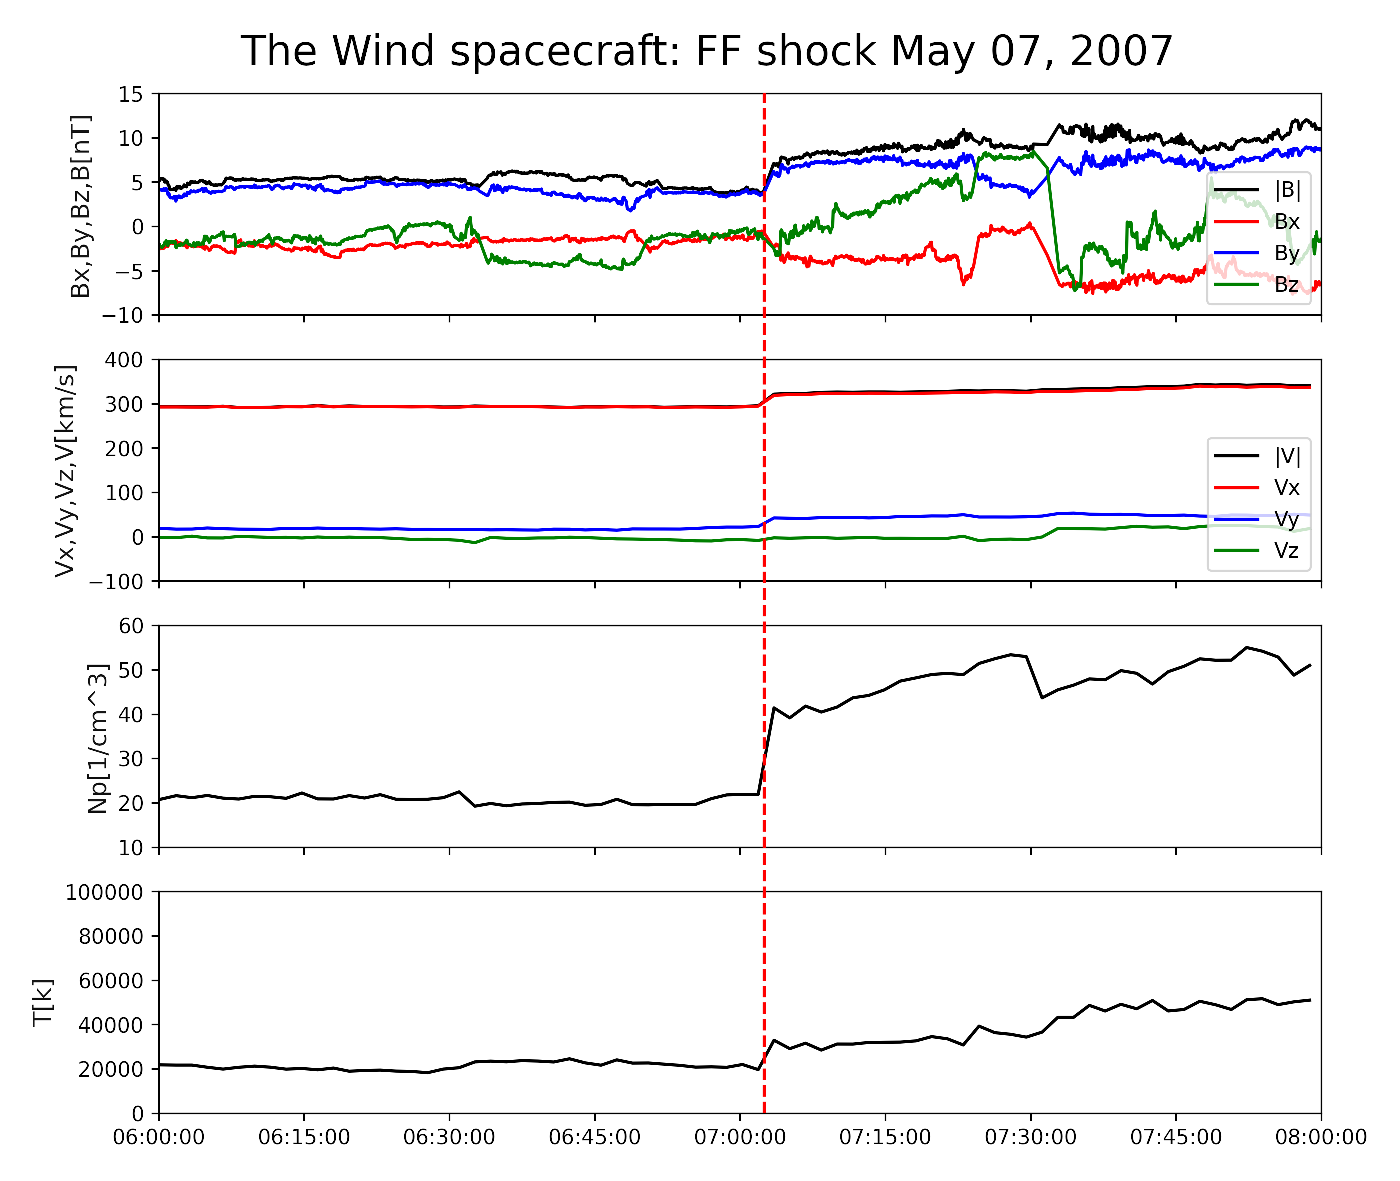
\includegraphics[width=1.\textwidth]{jgr-2023-ipshocks-f01.eps}
\caption{The plot of the shock detected by the Wind spacecraft on May 7, 2007, at 07:02:30 (UTC). FF stands for the fast forward shock, which means the shock is traveling away from its driver. The panels show from top to bottom, the magnetic field magnitude as well as its components, the total velocity, and its components, density, and temperature. The dashed red line represents the exact shock time. The duration of the plot is two hours.}
\label{fig:WindIP0507}
\end{figure}

\pagebreak

\begin{figure}[!t]
\centering
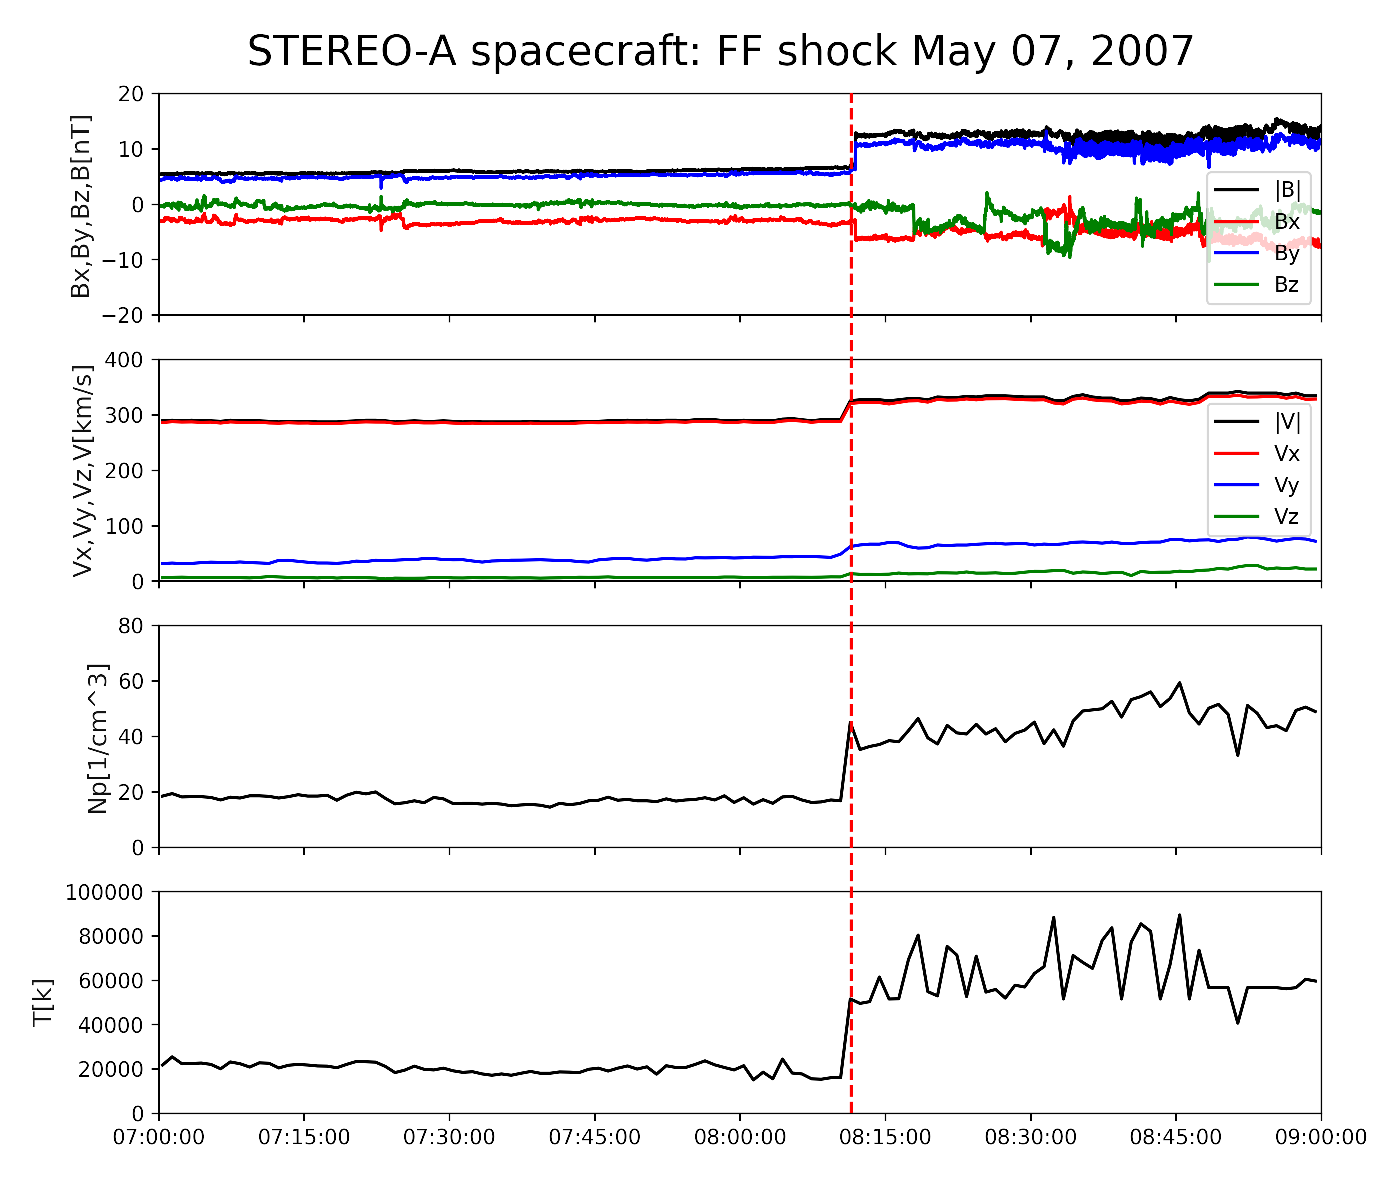
\includegraphics[width=1.\textwidth]{jgr-2023-ipshocks-f02.eps}
\caption{The plot of the shock detected by the STEREO$-$A spacecraft on May 7, 2007, at 08:11:30 (UTC). The symbols and details of the figures are the same as \ref{fig:WindIP0507}. The duration of the plot is two hours.}
\label{fig:staIP0507}
\end{figure}

\pagebreak

\begin{figure}[!t]
\centering
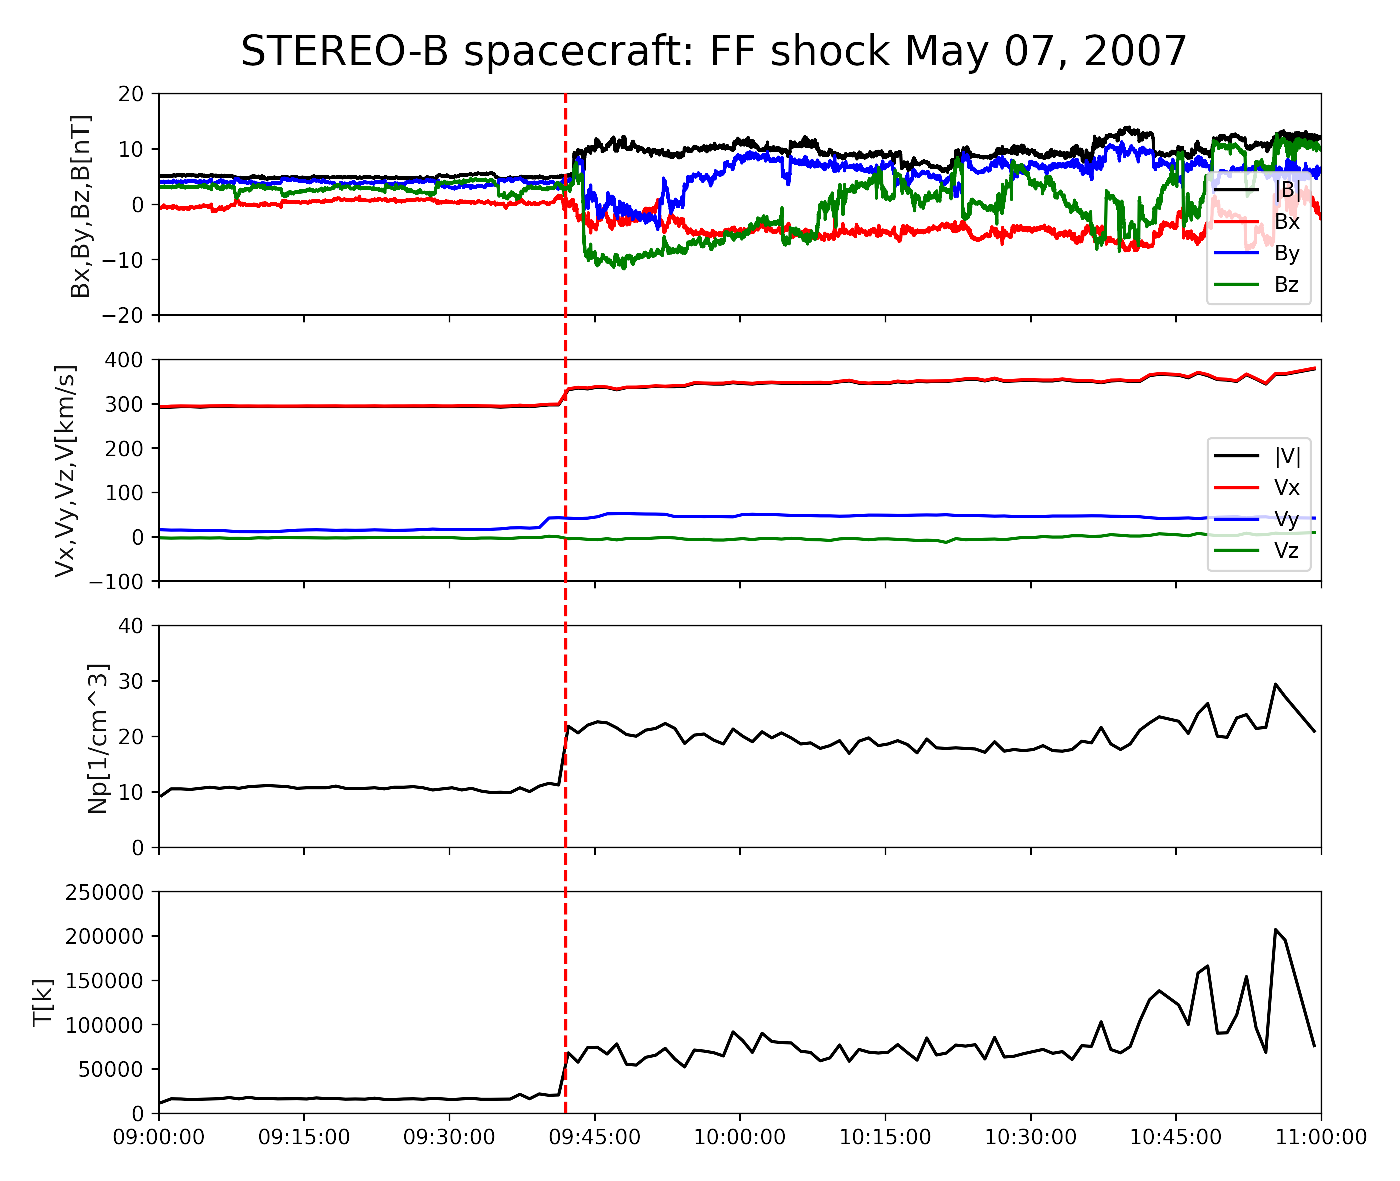
\includegraphics[width=1.\textwidth]{jgr-2023-ipshocks-f03.eps}
\caption{The plot of the shock detected by the STEREO$-$B spacecraft on May 7, 2007, at {09:42:00} (UTC). The symbols and details of the figures are the same as \ref{fig:WindIP0507}. The duration of the plot is two hours.}
\label{fig:stbIP0507}
\end{figure}

\pagebreak

\begin{figure}[!t]
\centering
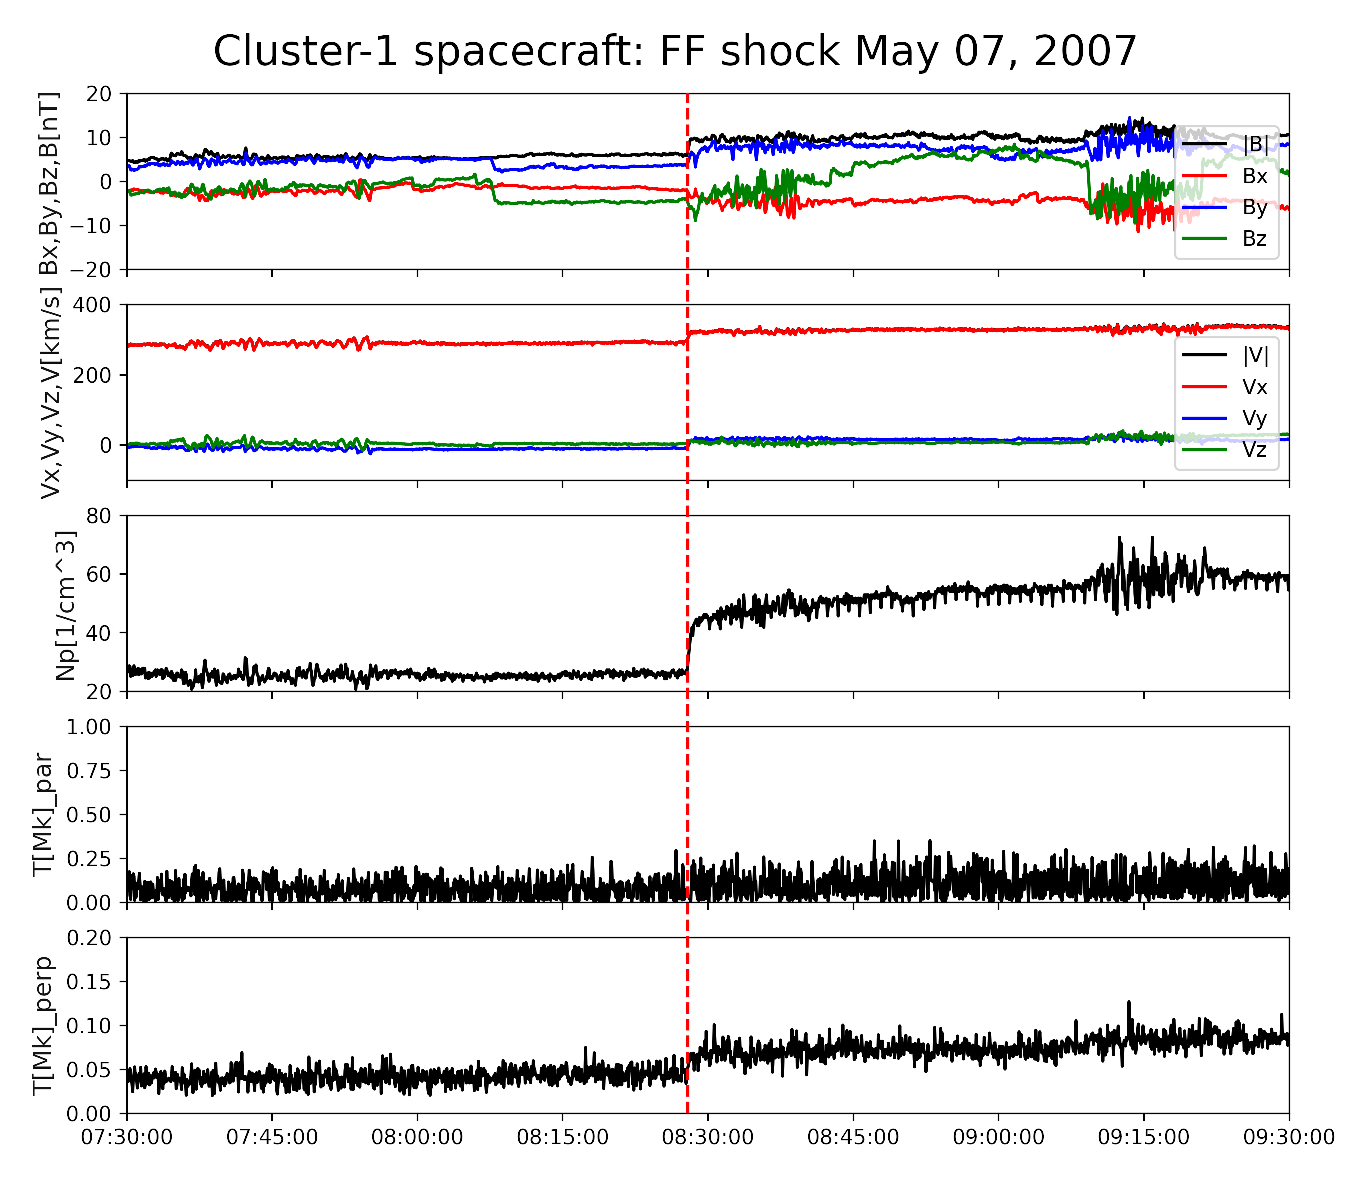
\includegraphics[width=1.\textwidth]{jgr-2023-ipshocks-f04.eps}
\caption{The plot of the shock detected by the Cluster SC1 on May 7, 2007, at 08:27:55 (UTC). The panels show from top to bottom, the magnetic field magnitude as well as its components, the total velocity, and its components, density, and parallel and perpendicular temperatures. The dashed red line represents the exact shock time. The duration of the plot is two hours.}
\label{fig:cl10507}
\end{figure}

\pagebreak

\begin{figure}[!t]
\centering
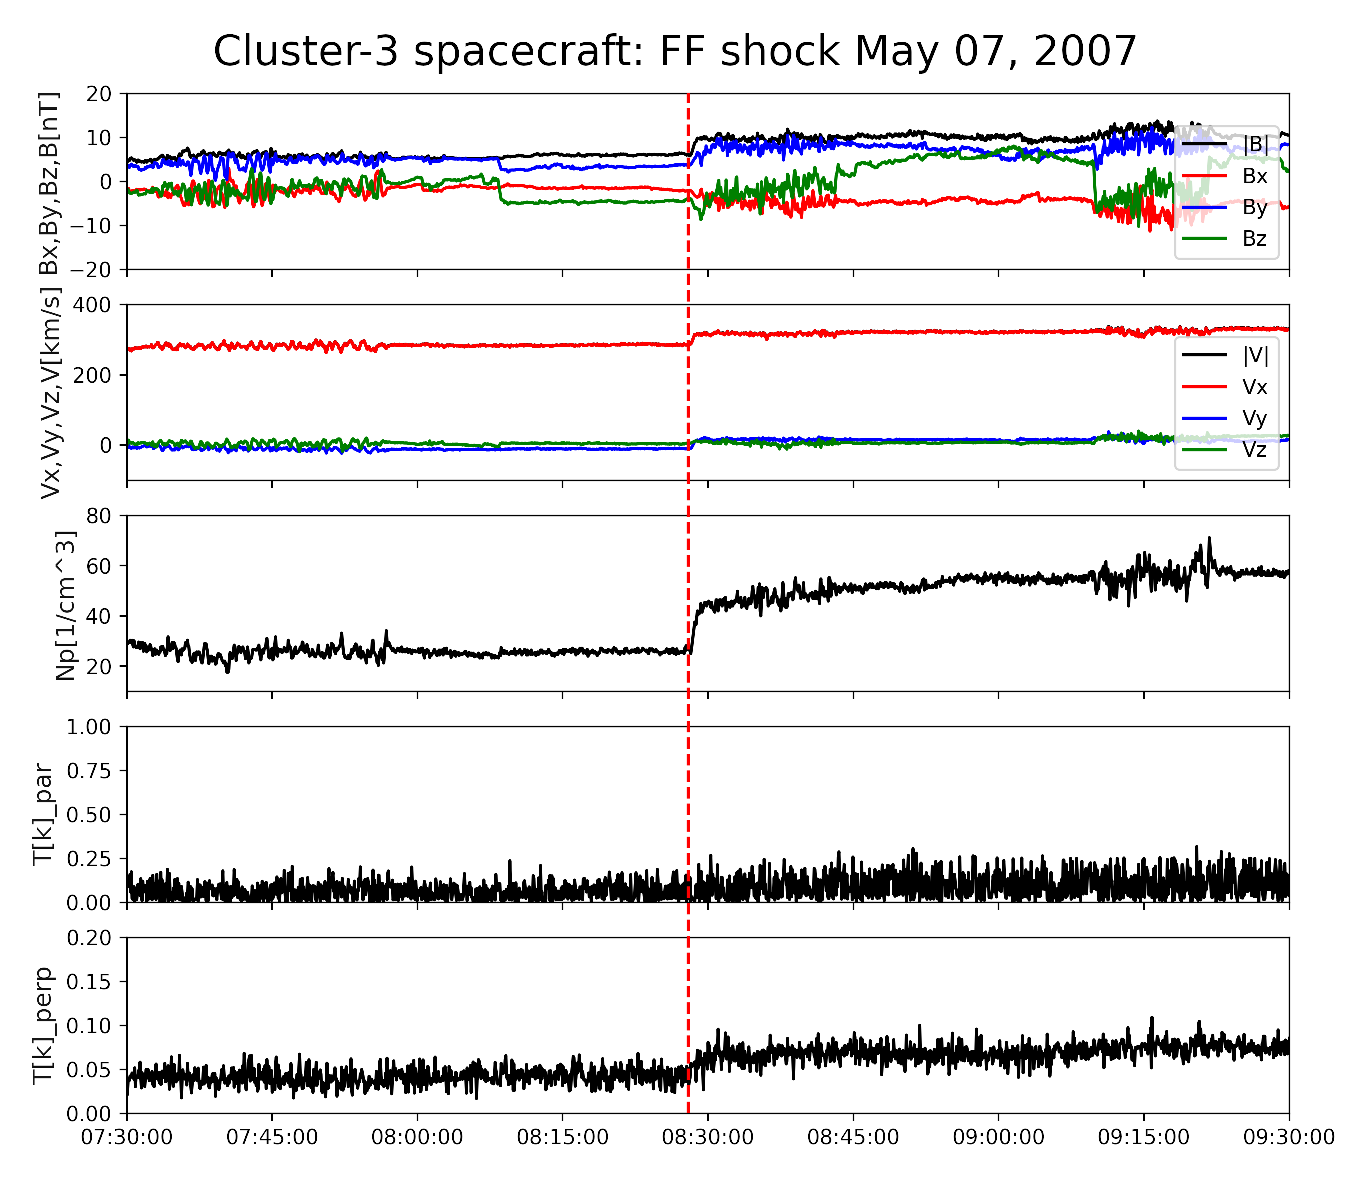
\includegraphics[width=1.\textwidth]{jgr-2023-ipshocks-f05.eps}
\caption{The plot of the shock detected by the Cluster SC3 on May 7, 2007, at 08:28:00 (UTC). The symbols and details of the figures are the same as \ref{fig:cl10507}. The duration of the plot is two hours.}
\label{fig:cl30507}
\end{figure}

\pagebreak

\begin{figure}[!t]
\centering
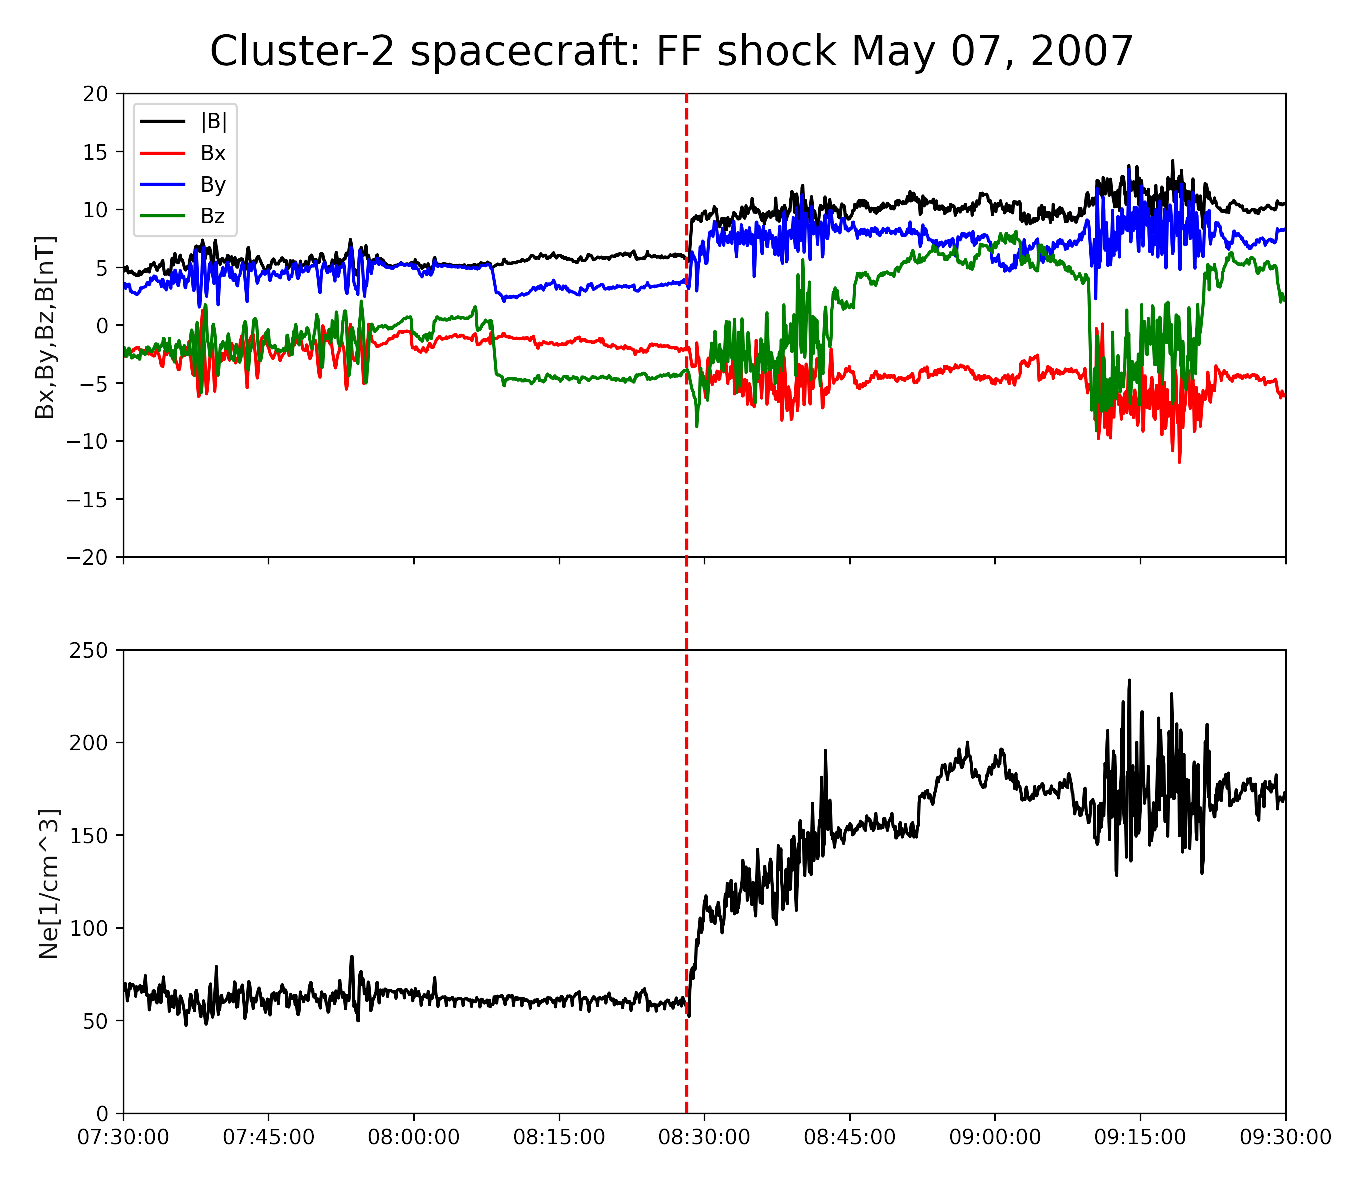
\includegraphics[width=1.\textwidth]{jgr-2023-ipshocks-f06.eps}
\caption{The plot of the shock detected by the Cluster SC2 on May 7, 2007, at 08:28:10 (UTC). The panels show from top to bottom, the magnetic field magnitude as well as its components, and the obtained electron density from the spacecraft potential. The dashed red line represents the exact shock time. The duration of the plot is two hours.}
\label{fig:cl20507}
\end{figure}

\pagebreak

\begin{figure}[!t]
\centering
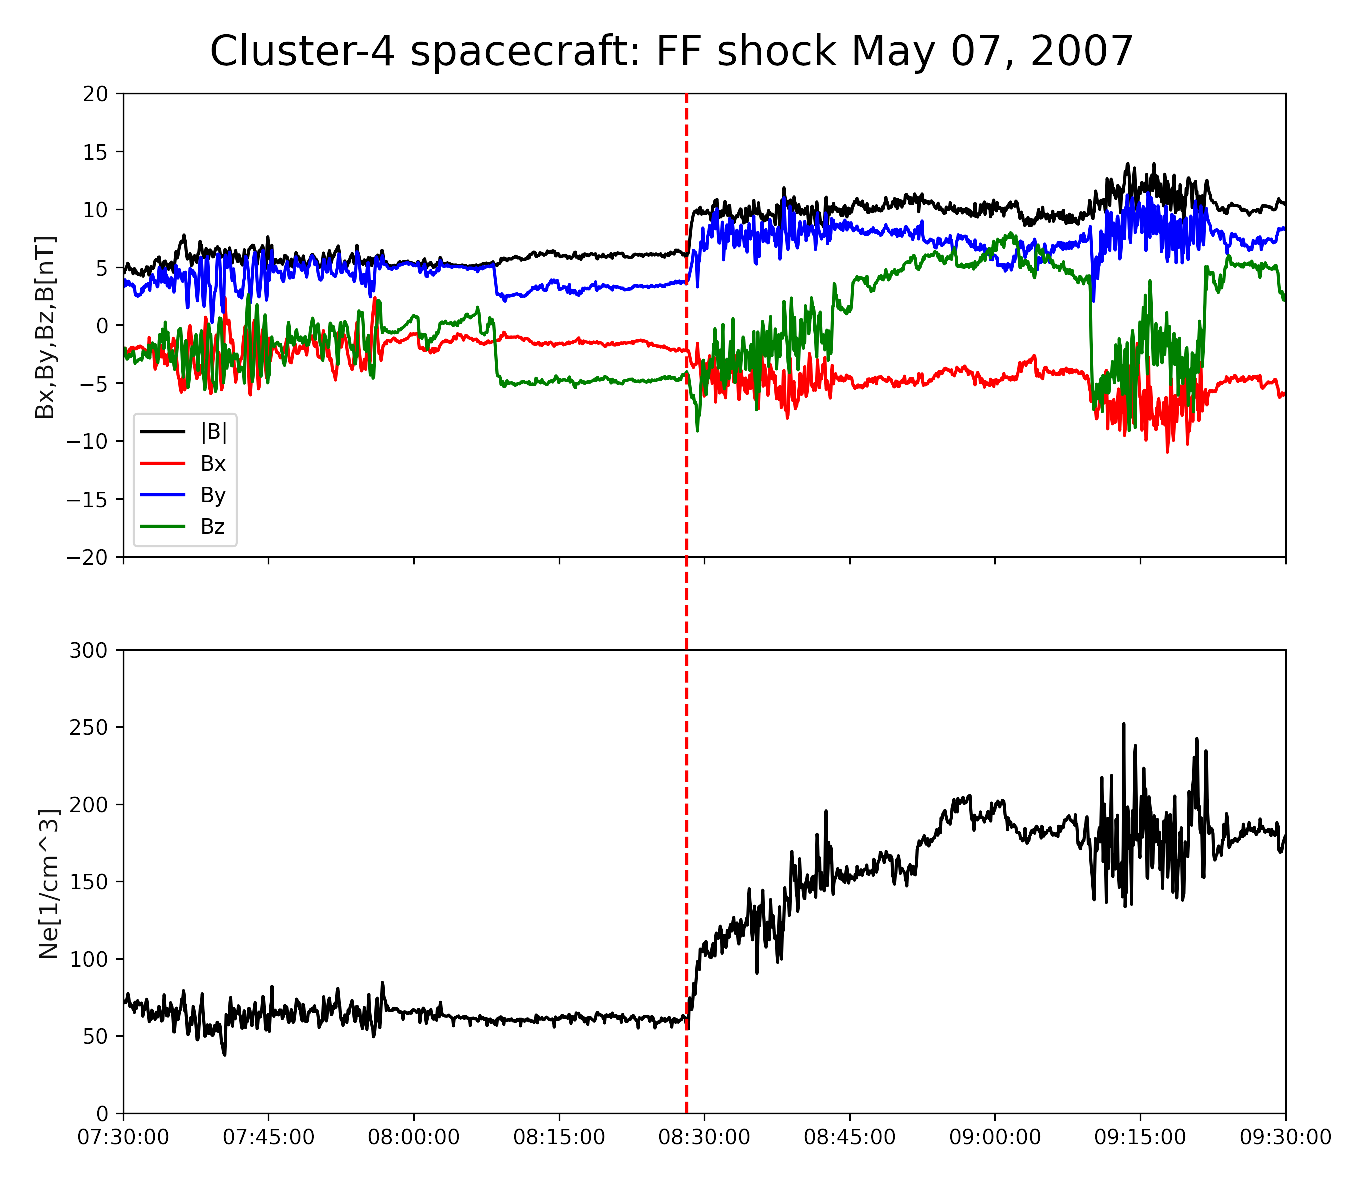
\includegraphics[width=1.\textwidth]{jgr-2023-ipshocks-f07.eps}
\caption{The plot of the shock detected by the Cluster SC4 on May 7, 2007, at 08:28:10 (UTC). The symbols and details of the figures are the same as \ref{fig:cl20507}. The duration of the plot is two hours.}
\label{fig:cl40507}
\end{figure}

\pagebreak

\begin{figure}[!t]
\centering
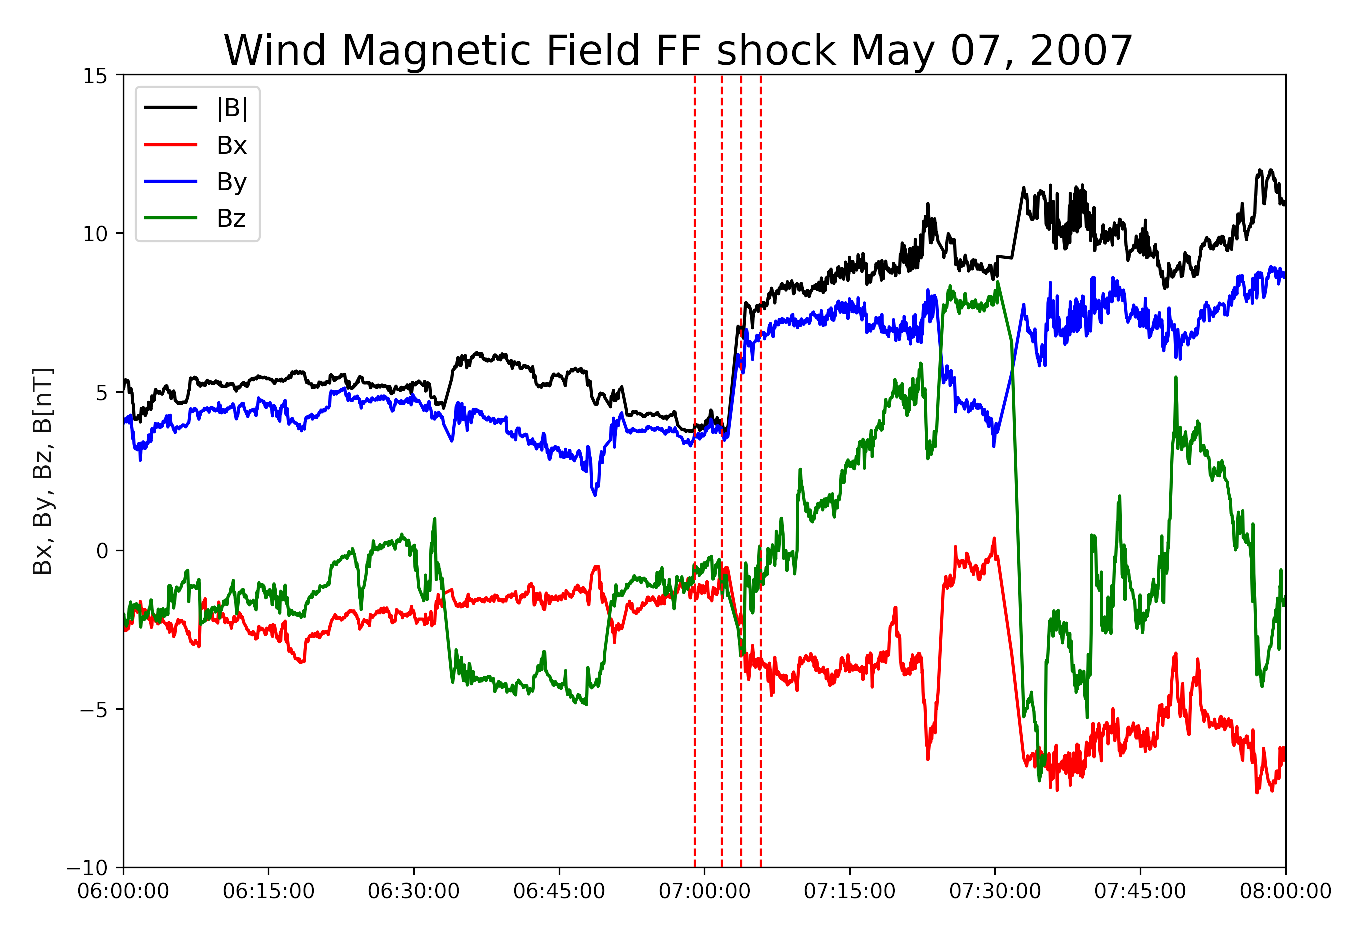
\includegraphics[width=1\textwidth]{jgr-2023-ipshocks-f08.eps}
\caption{The Wind magnetic field measurements. The upstream $\Delta t_{up}$ is between (06:59:00 - 07:01:47), and the downstream $\Delta t_{down}$ is between (07:03:50 - 07:05:50). FF stands for the fast forward shock, which means the shock is traveling away from its driver. The chosen intervals of the upstream and downstream magnetic field. The red dashed lines each represent the upstream starting time and ending time and the downstream starting time and ending time, respectively}
\label{fig:WindB}
\end{figure}

\pagebreak

\begin{figure}[!t]
\centering
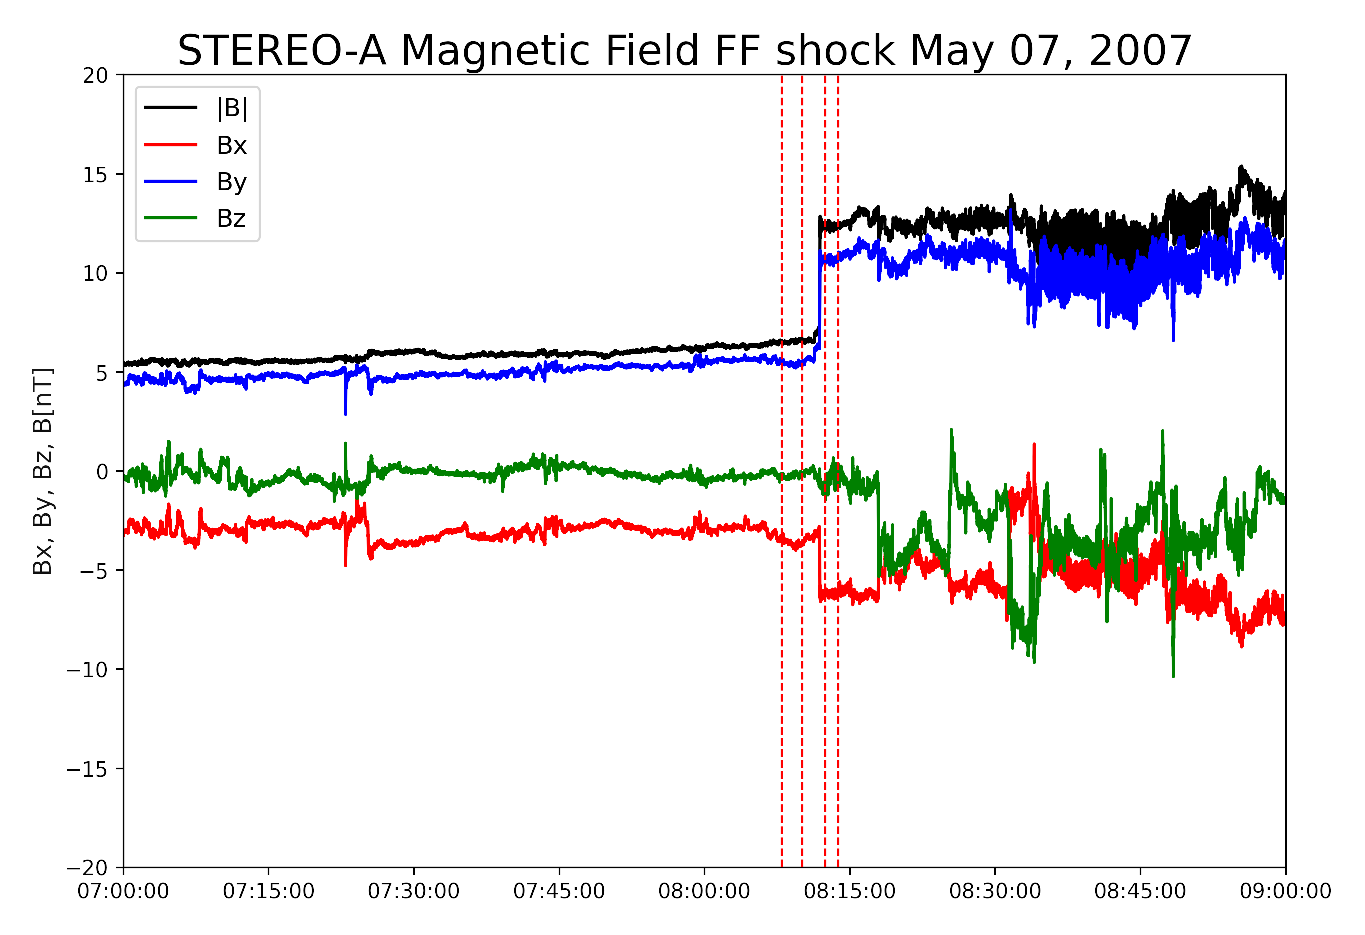
\includegraphics[width=1\textwidth]{jgr-2023-ipshocks-f09.eps}
\caption{The STEREO$-$A magnetic field measurements. The upstream $\Delta t_{up}$ is between (08:08:00 - 08:10:05), and the downstream $\Delta t_{down}$ is between (08:12:30 - 08:13:50). The symbols and details of the figures are the same as \ref{fig:WindB}}
\label{fig:staB}
\end{figure}

\pagebreak

\begin{figure}[!t]
\centering
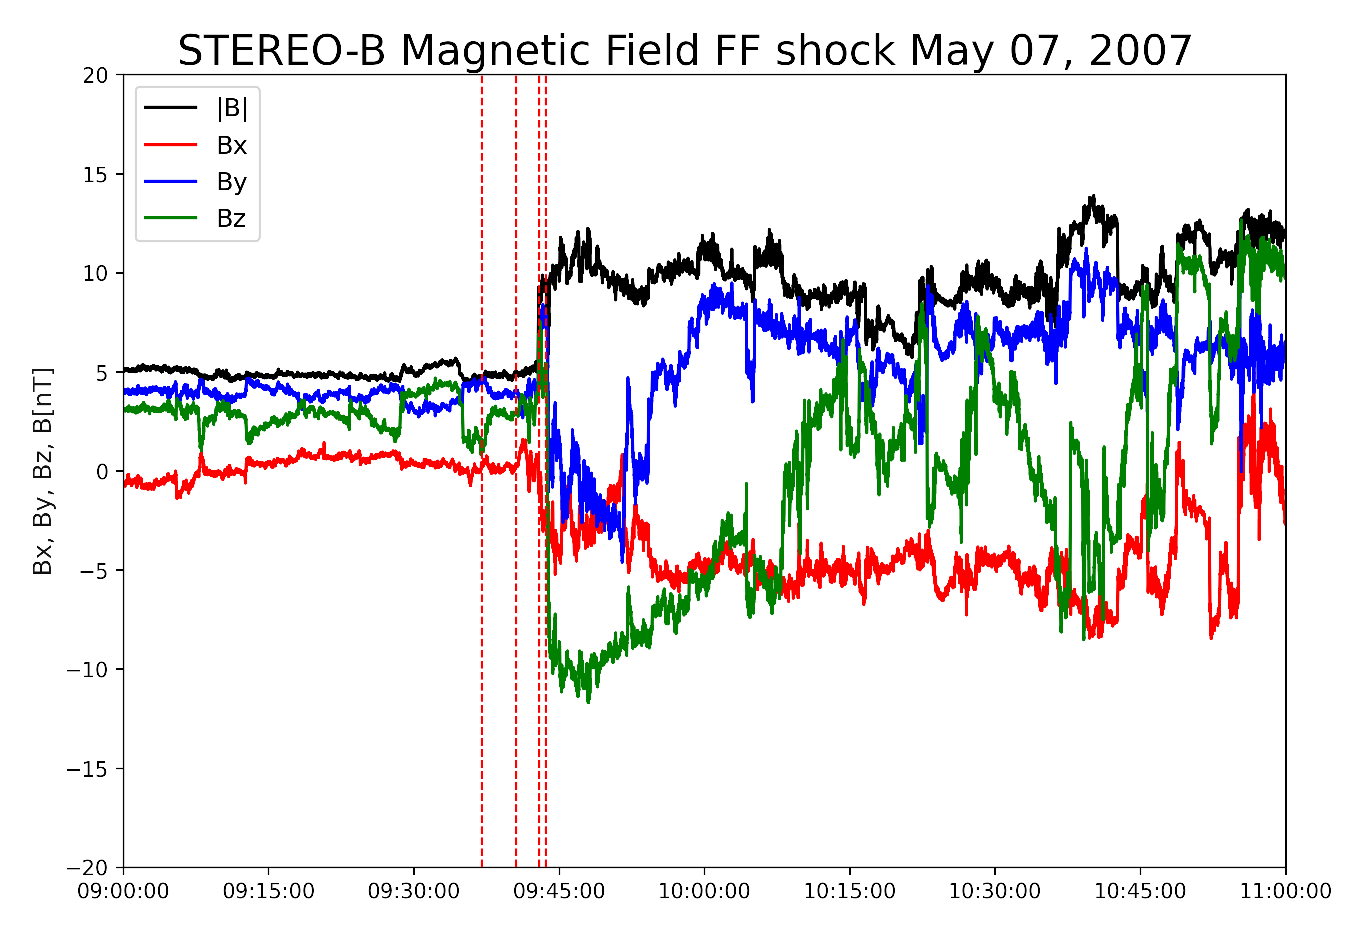
\includegraphics[width=1.\textwidth]{jgr-2023-ipshocks-f10.eps}
\caption{The STEREO$-$B magnetic field measurements. The upstream $\Delta t_{up}$ is between (09:37:00 - 09:40:35), and the downstream $\Delta t_{down}$ is between (09:42:57 - 09:43:38). The symbols and details of the figures are the same as \ref{fig:WindB}}
\label{fig:stbB}
\end{figure}

\pagebreak

\begin{figure}[!t]
\centering
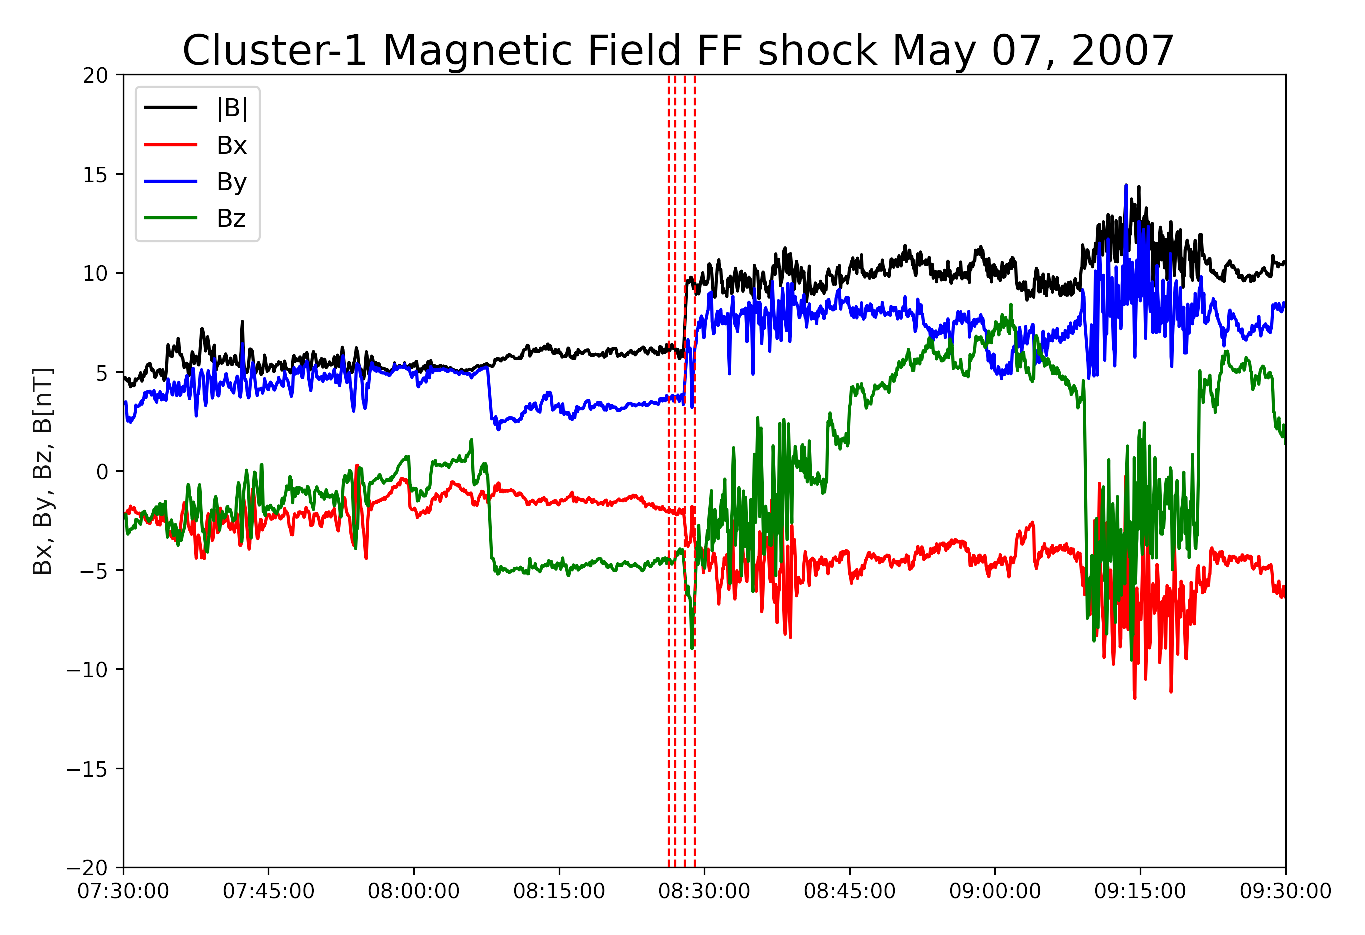
\includegraphics[width=1.\textwidth]{jgr-2023-ipshocks-f11.eps}
\caption{The Cluster-1 B magnetic field measurements. The upstream $\Delta t_{up}$ is between (08:26:10 - 08:27:00), and the downstream $\Delta t_{down}$ is between (08:28:00 - 08:29:00). The symbols and details of the figures are the same as \ref{fig:WindB}}
\label{fig:cl1b}
\end{figure}

\pagebreak

\begin{figure}[!t]
\centering
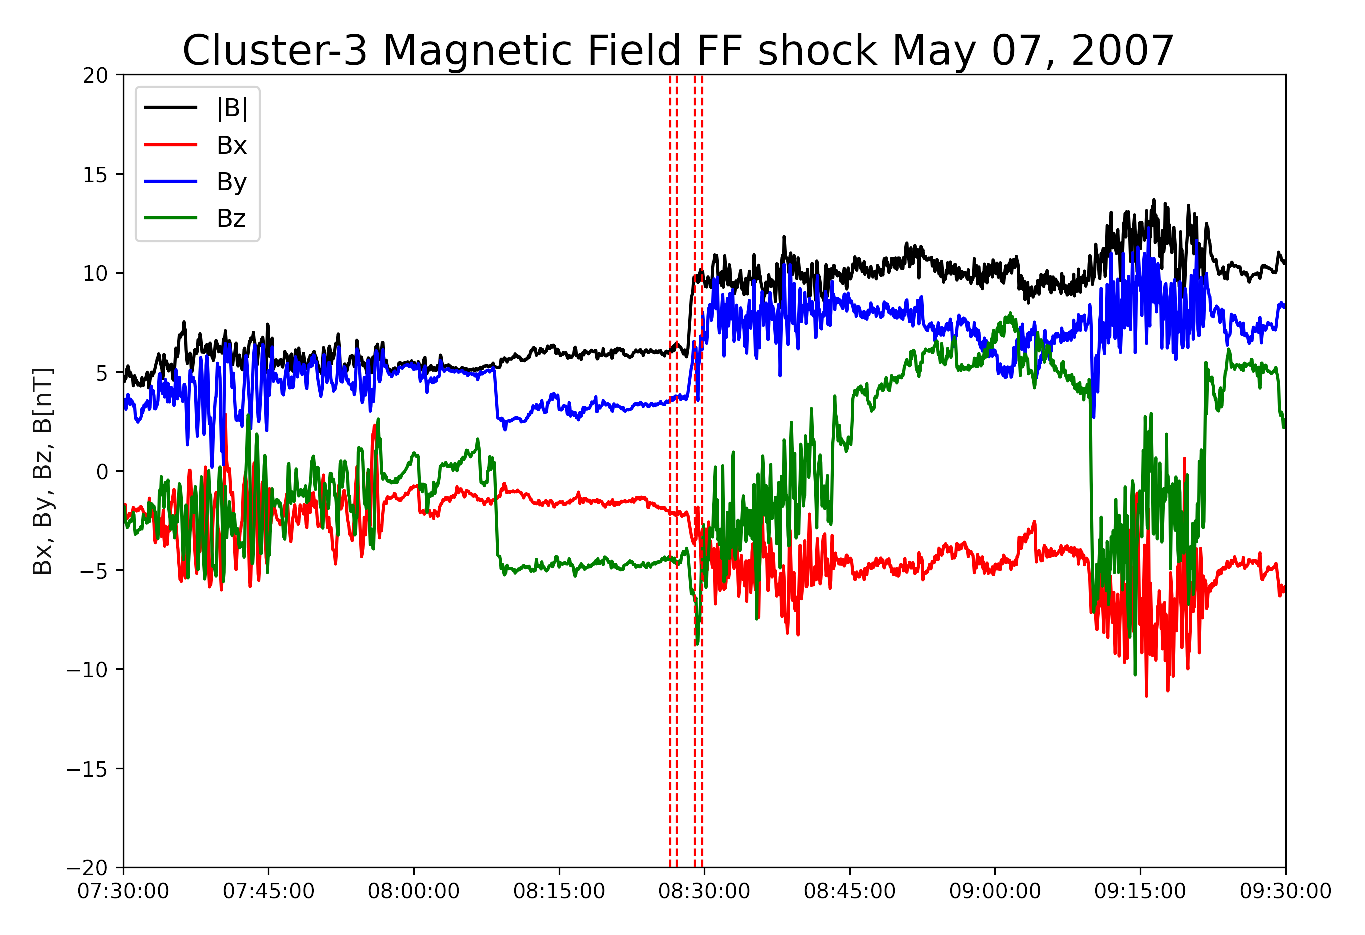
\includegraphics[width=1.\textwidth]{jgr-2023-ipshocks-f12.eps}
\caption{The Cluster-3 B magnetic field measurements. The upstream $\Delta t_{up}$ is between (08:26:30 - 08:27:10), and the downstream $\Delta t_{down}$ is between (08:29:00 - 08:29:47). The symbols and details of the figures are the same as \ref{fig:WindB}}
\label{fig:cl3b}
\end{figure}

\pagebreak

\begin{figure}[!t]
\centering
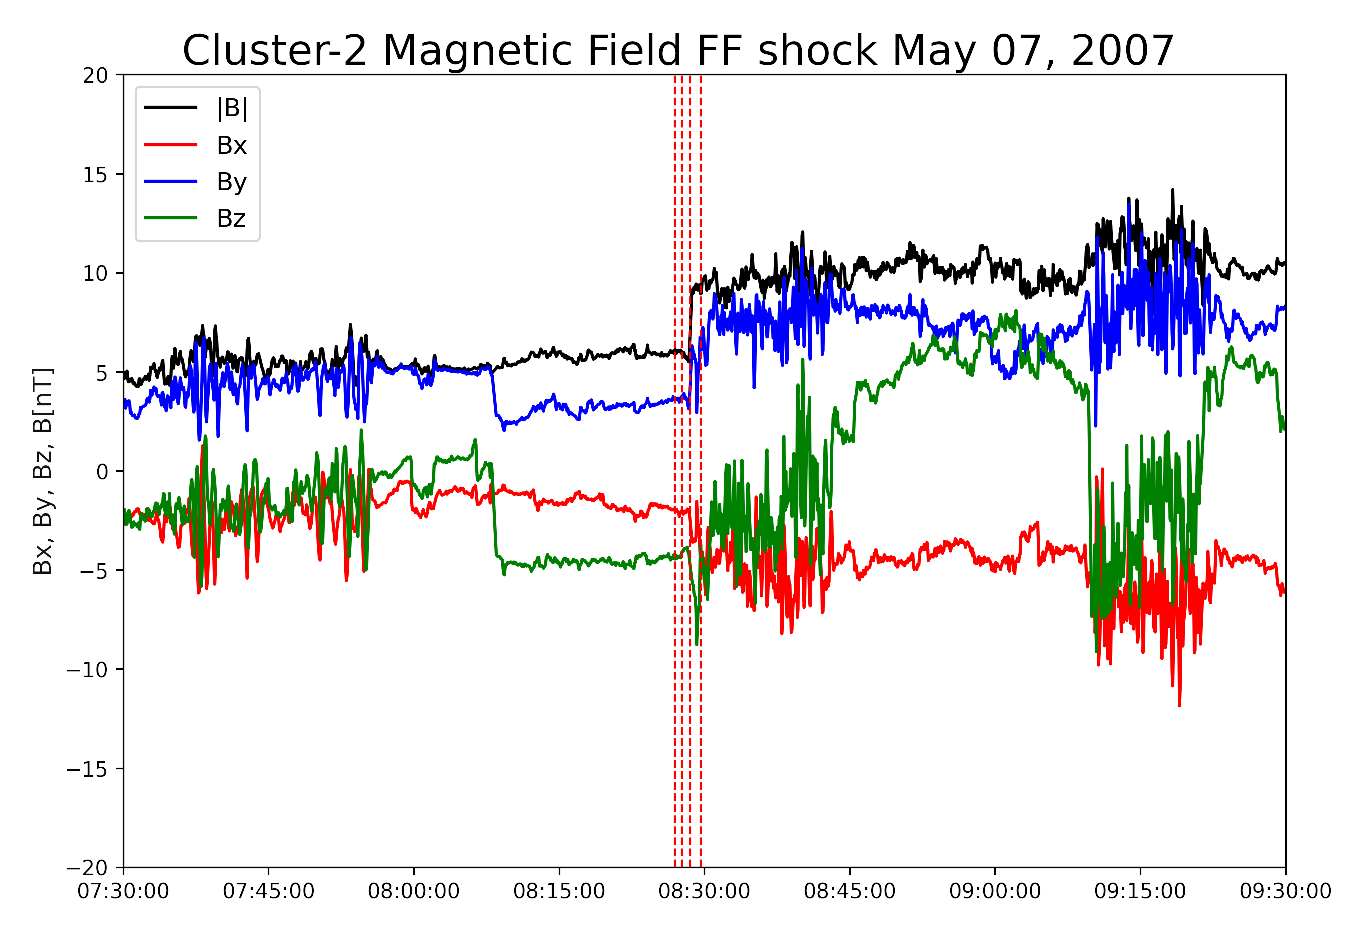
\includegraphics[width=1\textwidth]{jgr-2023-ipshocks-f13.eps}
\caption{The Cluster-2 B magnetic field measurements. The upstream $\Delta t_{up}$ is between (08:26:56 - 08:27:40), and the downstream $\Delta t_{down}$ is between (08:28:32 - 08:29:37). The symbols and details of the figures are the same as \ref{fig:WindB}}
\label{fig:cl2b}
\end{figure}

\pagebreak

\begin{figure}[!t]
\centering
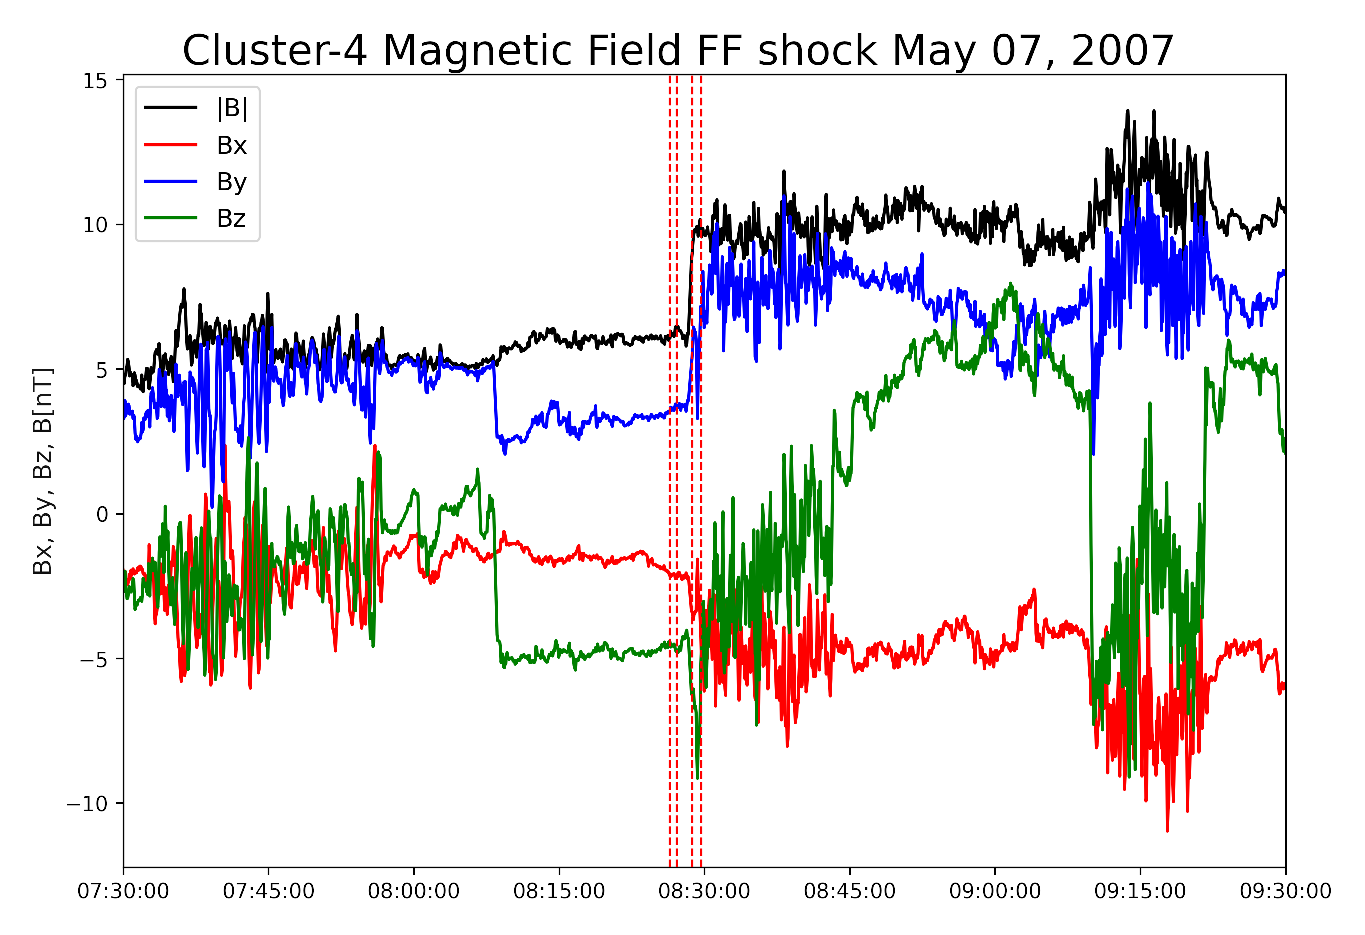
\includegraphics[width=1.\textwidth]{jgr-2023-ipshocks-f14.eps}
\caption{The Cluster-4 B magnetic field measurements. The upstream $\Delta t_{up}$ is between (08:26:25 - 08:27:10), and the downstream $\Delta t_{down}$ is between (08:28:45 - 08:29:40). The symbols and details of the figures are the same as \ref{fig:WindB}}
\label{fig:cl4b}
\end{figure}

\pagebreak


% \begin{figure}[!t]
%\centering
%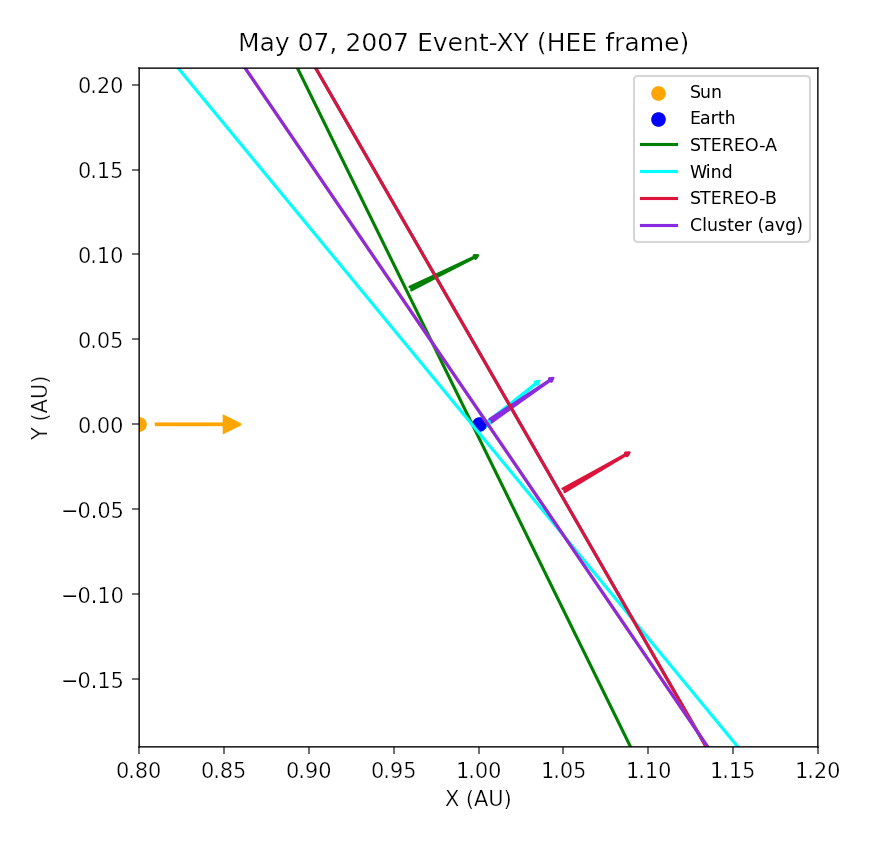
\includegraphics[width=.45\linewidth]{jgr-2023-ipshocks-f15a.eps}
%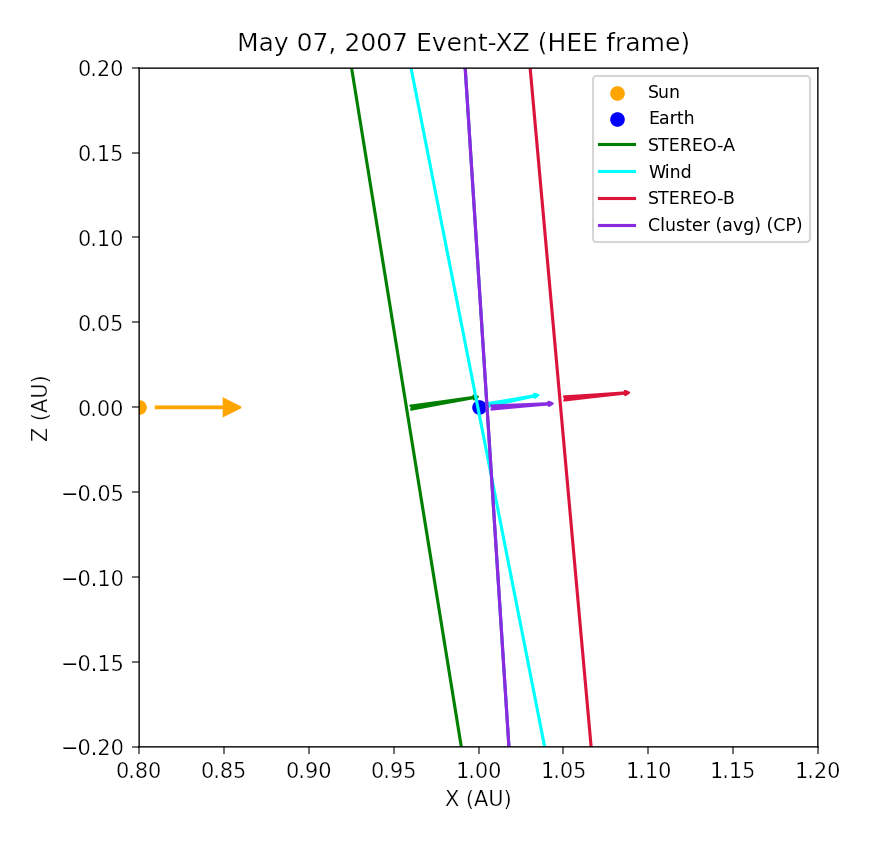
\includegraphics[width=.45\linewidth]{jgr-2023-ipshocks-f15b.eps}
%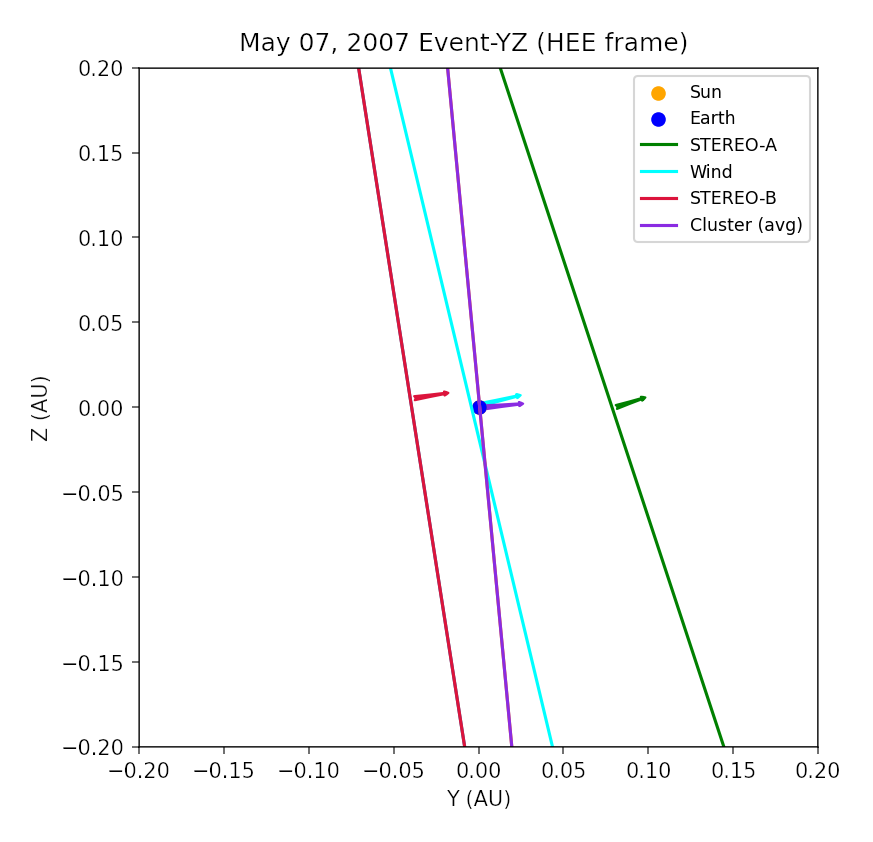
\includegraphics[width=.45\linewidth]{jgr-2023-ipshocks-f15c.eps}
%\caption{2D (Top left) XY, (Top right) XZ, and (Bottom) YZ sketches of the propagation of the IP shock through spacecraft-- Wind (light bluie), STEREO$-$A (green) and B (red), and average position of four Cluster satellites (purple). The orange arrow represents the Sun-Earth line direction. The arrows on spacecraft positions indicate the normal vector direction calculated from co-planarity method and the lines perpendicular to the normal vectors indicate the shock surface orientations. The sizes of the lines are arbitrary. The shock orientations for the four Cluster satellites are averaged.\label{fig:05072D}}
%\end{figure}

\begin{sidewaysfigure}
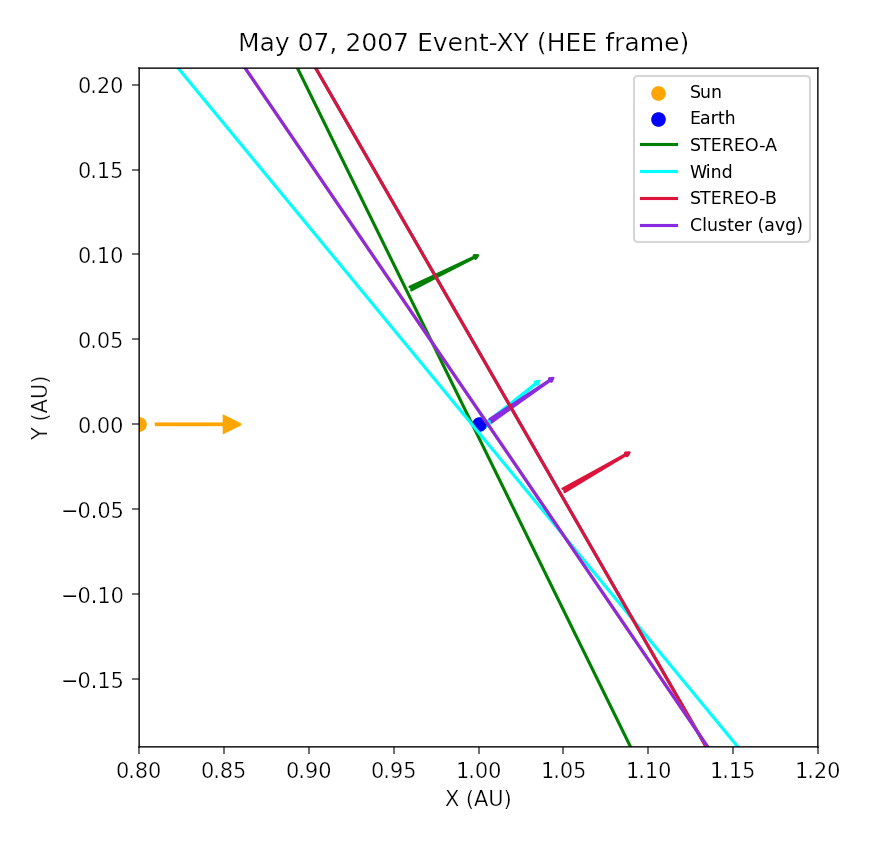
\includegraphics[width=.35\linewidth]{jgr-2023-ipshocks-f15a.eps}
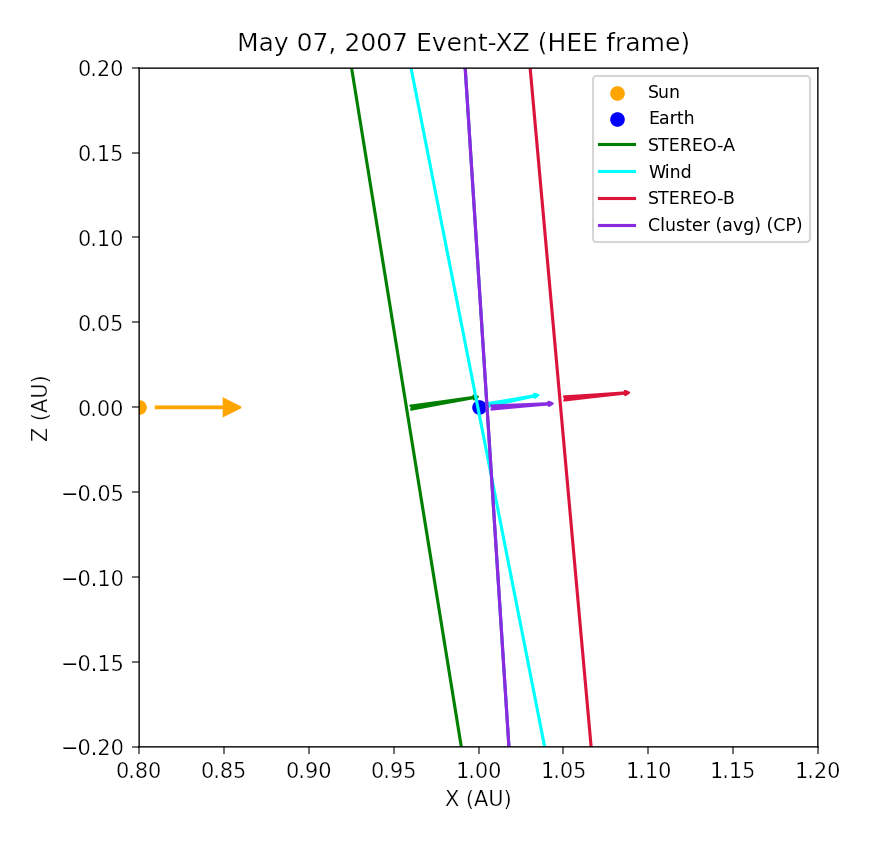
\includegraphics[width=.35\linewidth]{jgr-2023-ipshocks-f15b.eps}
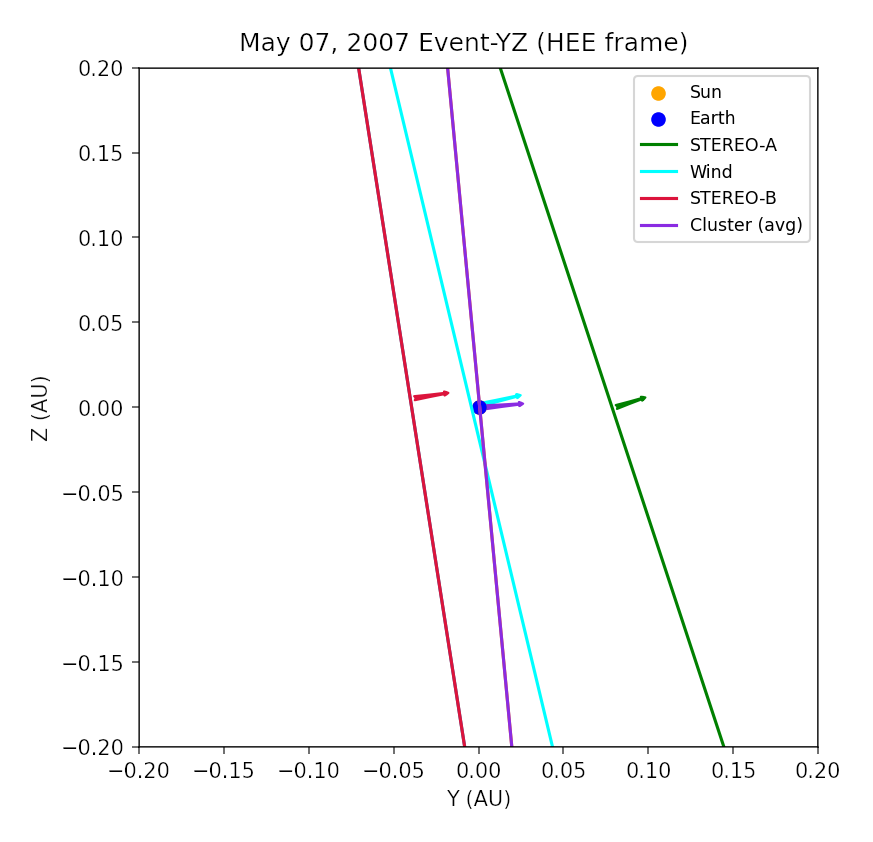
\includegraphics[width=.35\linewidth]{jgr-2023-ipshocks-f15c.eps}
\caption{2D (Top left) XY, (Top right) XZ, and (Bottom) YZ sketches of the propagation of the IP shock through spacecraft-- Wind (light bluie), STEREO$-$A (green) and B (red), and average position of four Cluster satellites (purple). The orange arrow represents the Sun-Earth line direction. The arrows on spacecraft positions indicate the normal vector direction calculated from co-planarity method and the lines perpendicular to the normal vectors indicate the shock surface orientations. The sizes of the lines are arbitrary. The shock orientations for the four Cluster satellites are averaged.\label{fig:05072D}}
\end{sidewaysfigure}

\pagebreak

% \begin{figure}[!t]
%\centering
%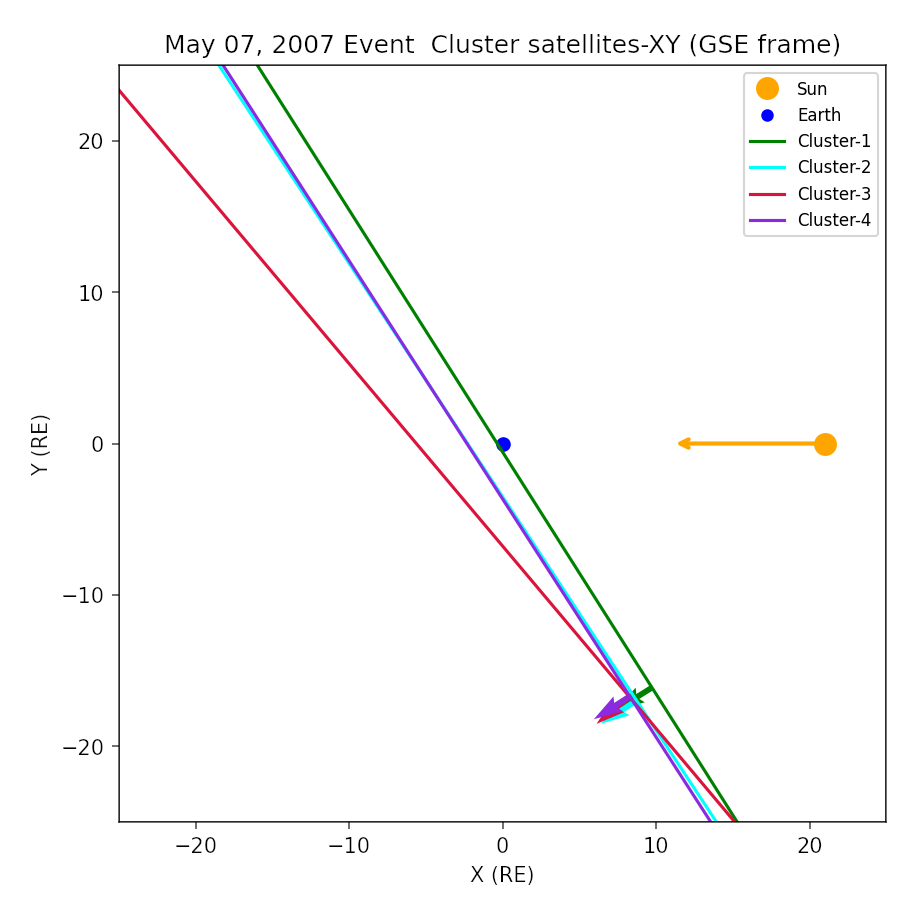
\includegraphics[width=.45\linewidth]{jgr-2023-ipshocks-f16a.eps}
%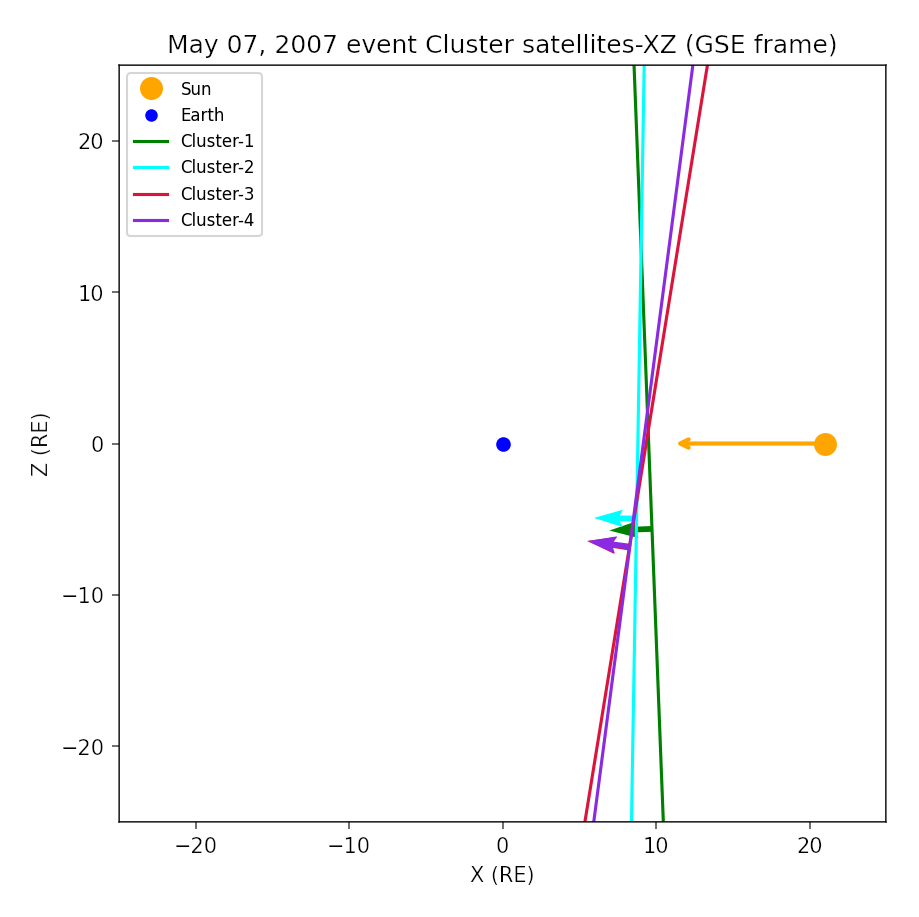
\includegraphics[width=.45\linewidth]{jgr-2023-ipshocks-f16b.eps}
%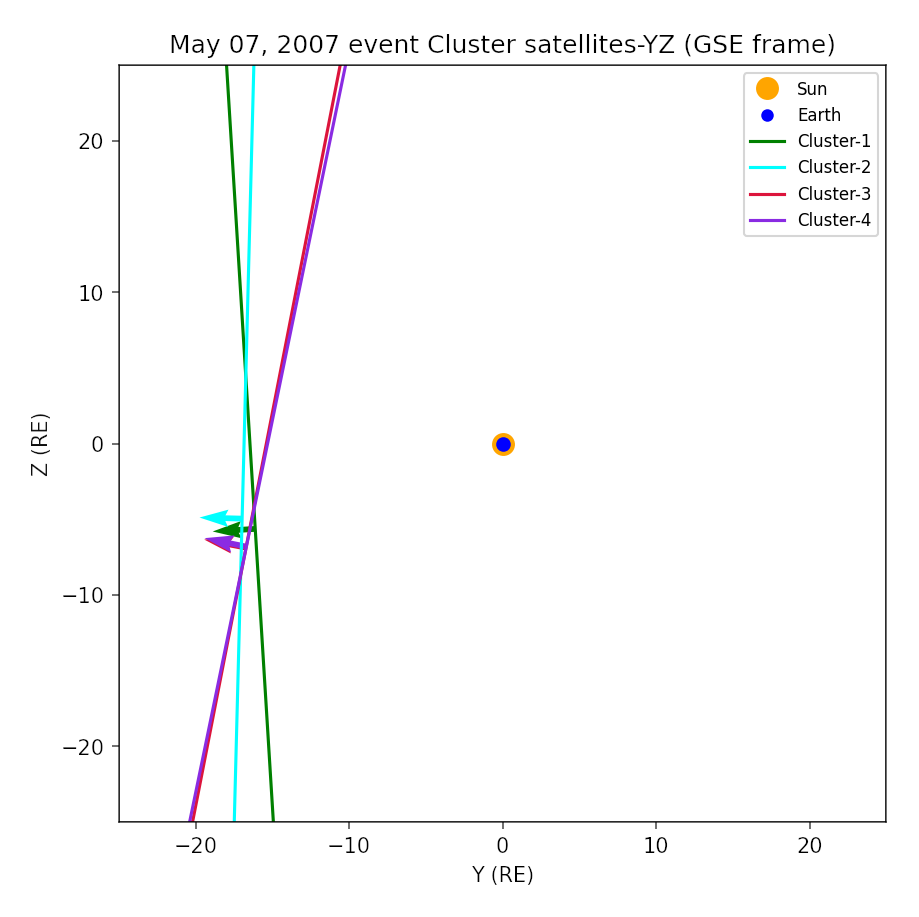
\includegraphics[width=.45\linewidth]{jgr-2023-ipshocks-f16c.eps}
%\caption{2D sketch in (Top left) XY, (Top right) XY, and (Bottom) YZ plans of the propagation of the IP shock through four Cluster satellites – SC1 (blue), SC2 (light blue), SC3 (purple), and SC4 (red). The orange arrow represents the Sun-Earth line direction. The arrows on spacecraft positions indicate the normal vector direction calculated from co-planaritiy and the lines perpendicular to the normal vectors indicate the shock surface orientations. The sizes of the lines are arbitrary.\label{fig:clustertogether}}
%\end{figure}

\begin{sidewaysfigure}
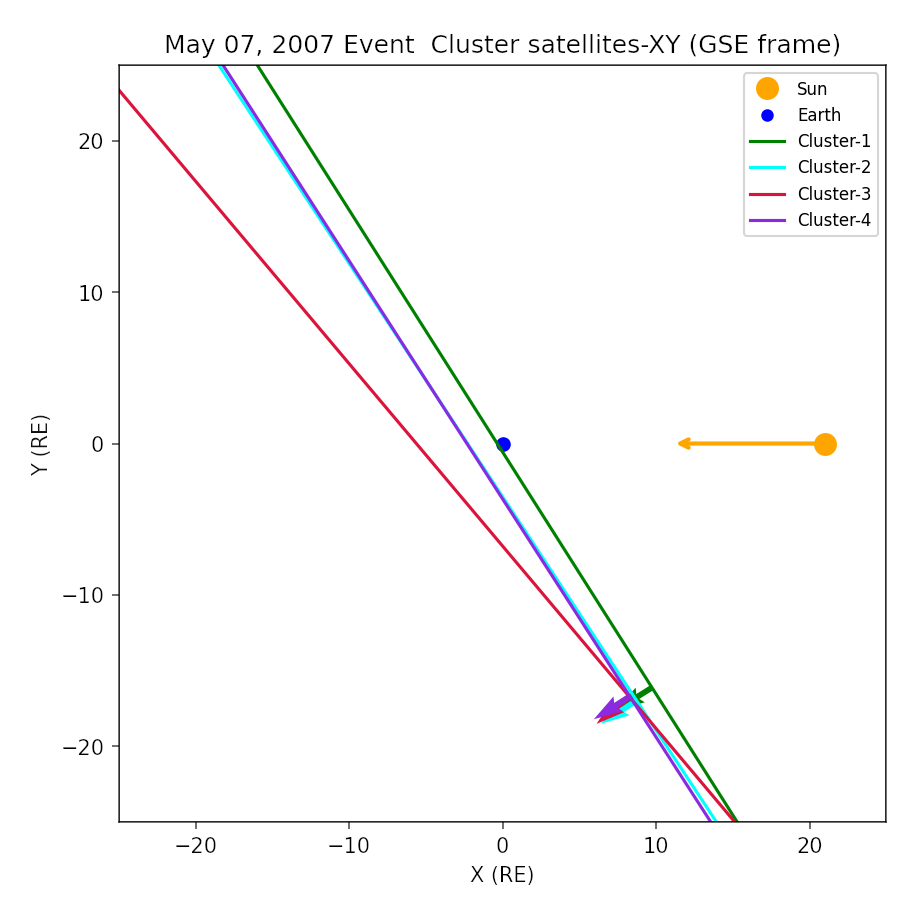
\includegraphics[width=.35\linewidth]{jgr-2023-ipshocks-f16a.eps}
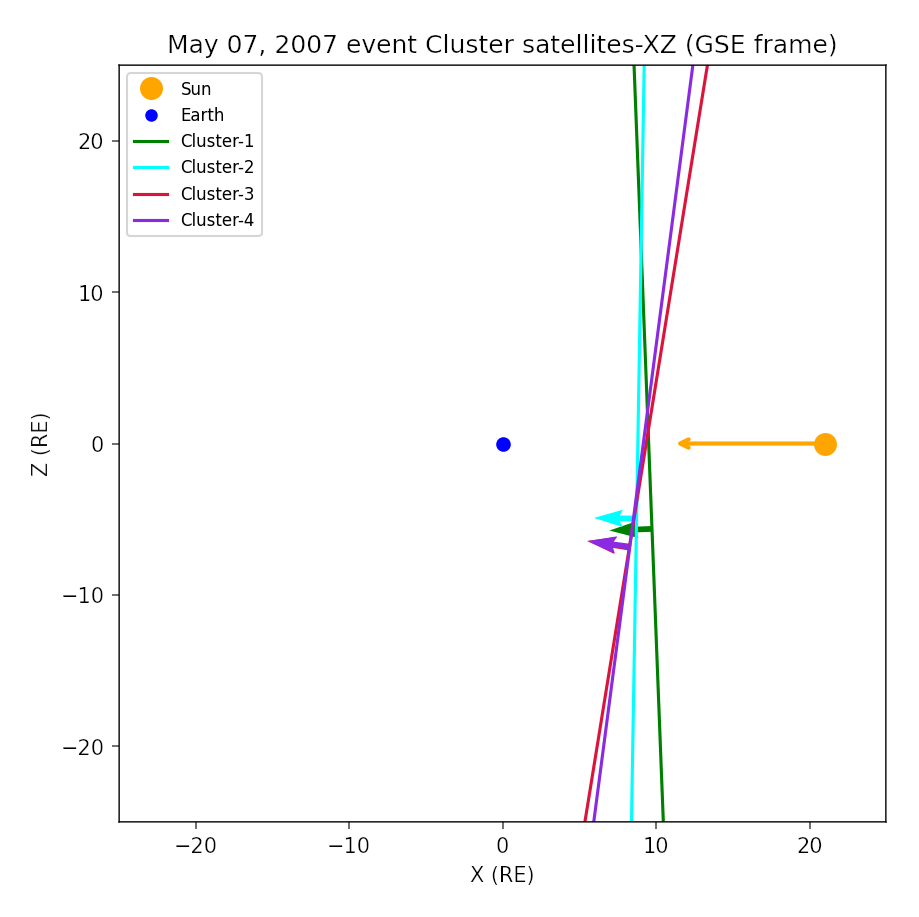
\includegraphics[width=.35\linewidth]{jgr-2023-ipshocks-f16b.eps}
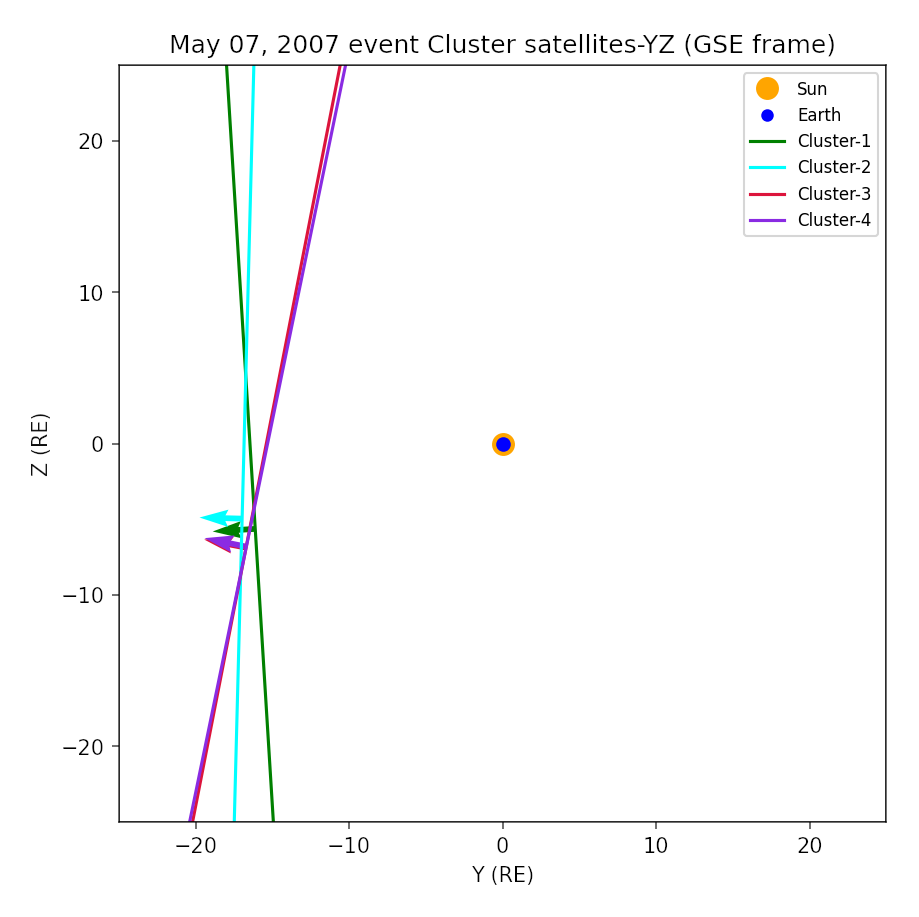
\includegraphics[width=.35\linewidth]{jgr-2023-ipshocks-f16c.eps}
\caption{2D sketch in (Top left) XY, (Top right) XY, and (Bottom) YZ plans of the propagation of the IP shock through four Cluster satellites – SC1 (blue), SC2 (light blue), SC3 (purple), and SC4 (red). The orange arrow represents the Sun-Earth line direction. The arrows on spacecraft positions indicate the normal vector direction calculated from co-planaritiy and the lines perpendicular to the normal vectors indicate the shock surface orientations. The sizes of the lines are arbitrary.\label{fig:clustertogether}}
\end{sidewaysfigure}

\pagebreak

% \begin{figure}[!t]
%\centering
%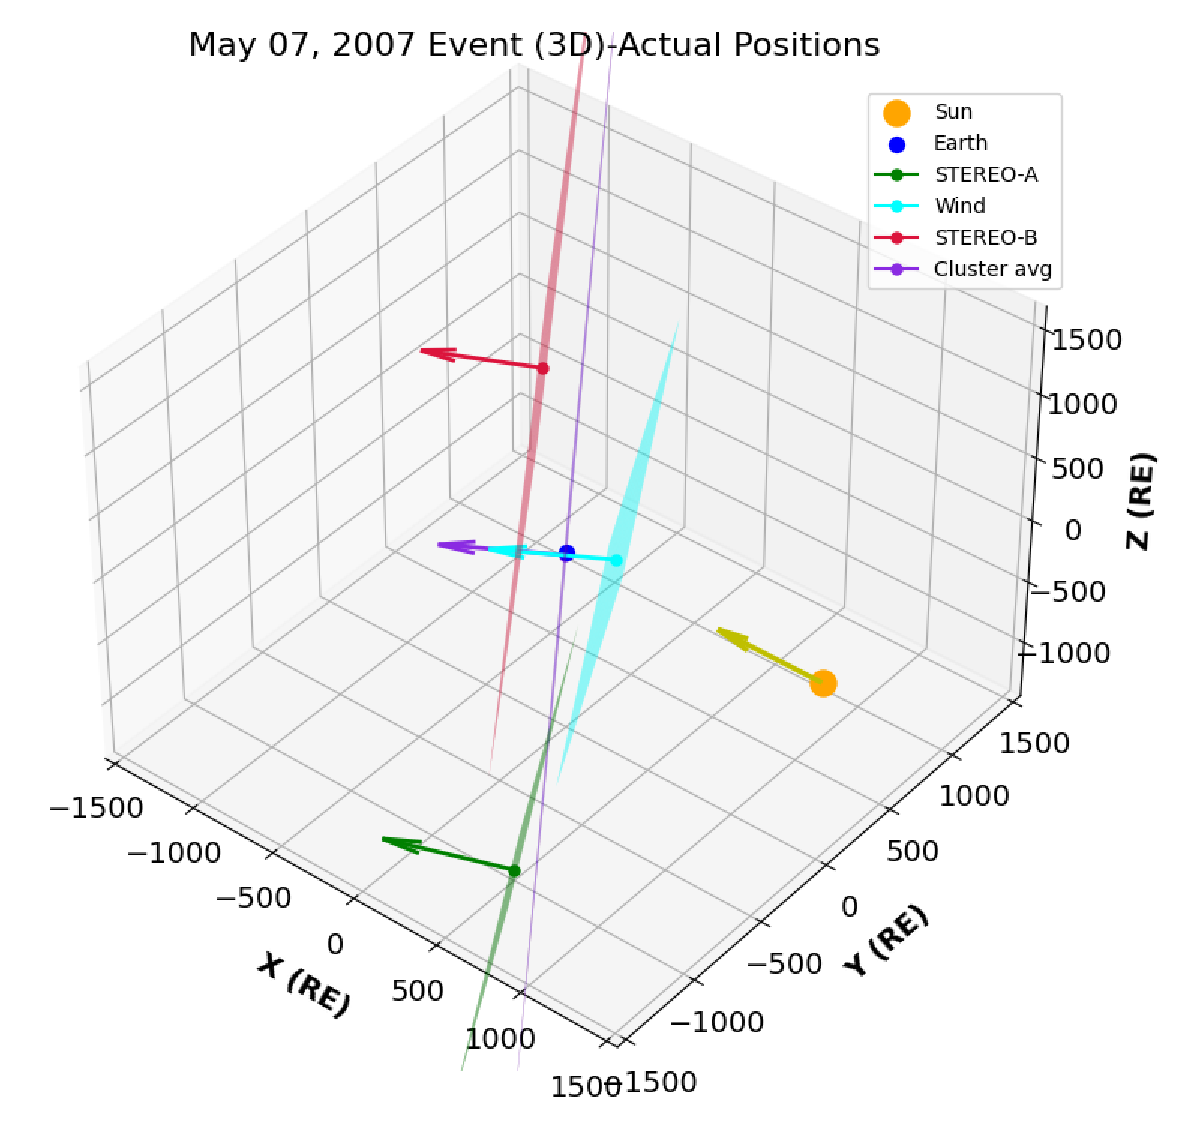
\includegraphics[width=.45\linewidth]{jgr-2023-ipshocks-f17a.eps}
%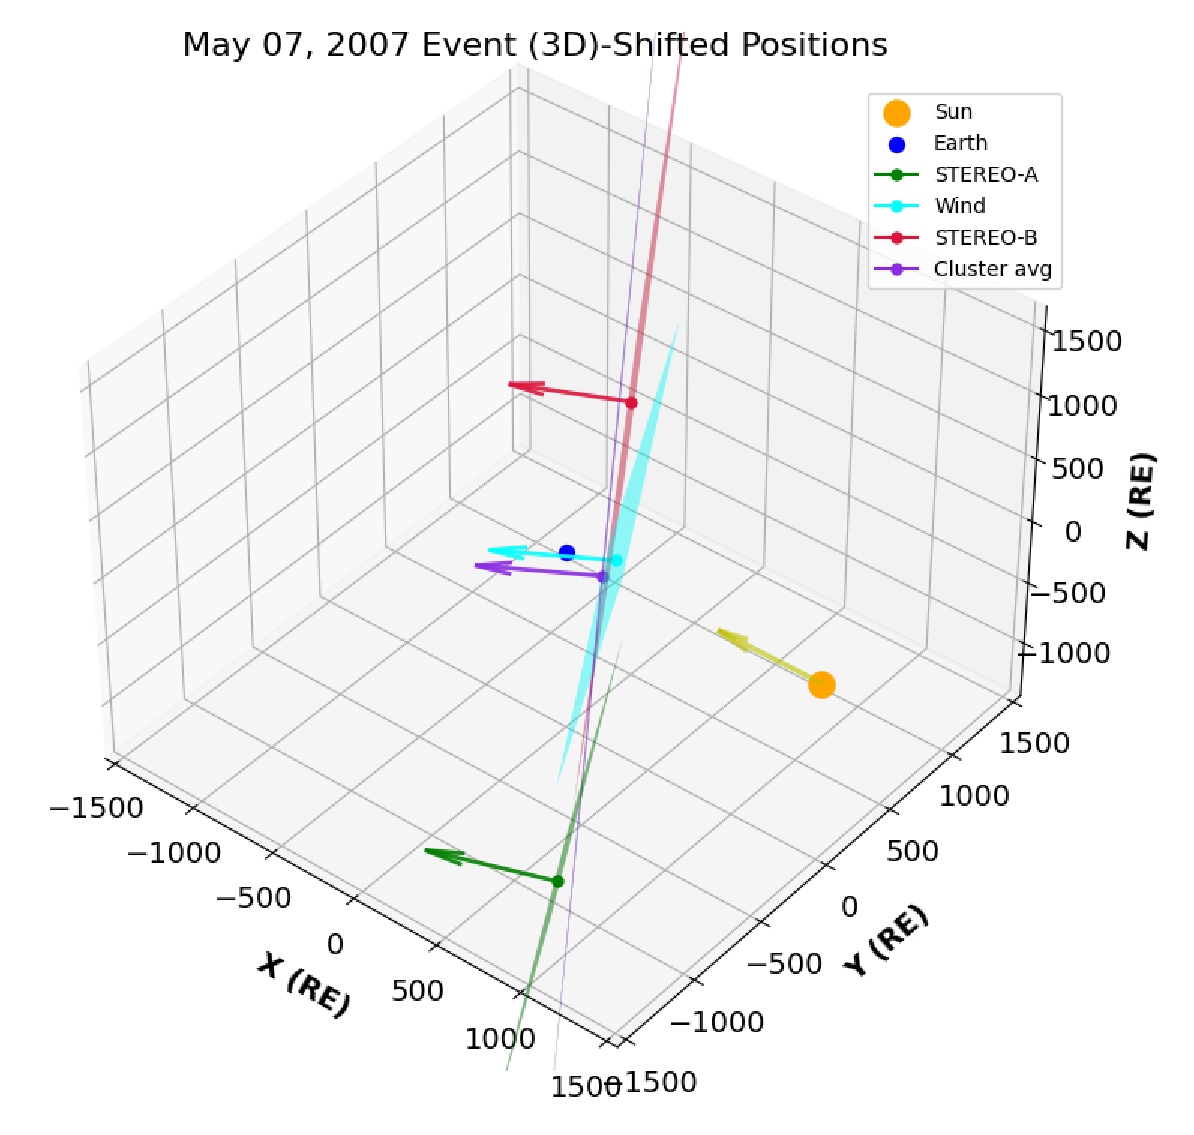
\includegraphics[width=.45\linewidth]{jgr-2023-ipshocks-f17b.eps} 
%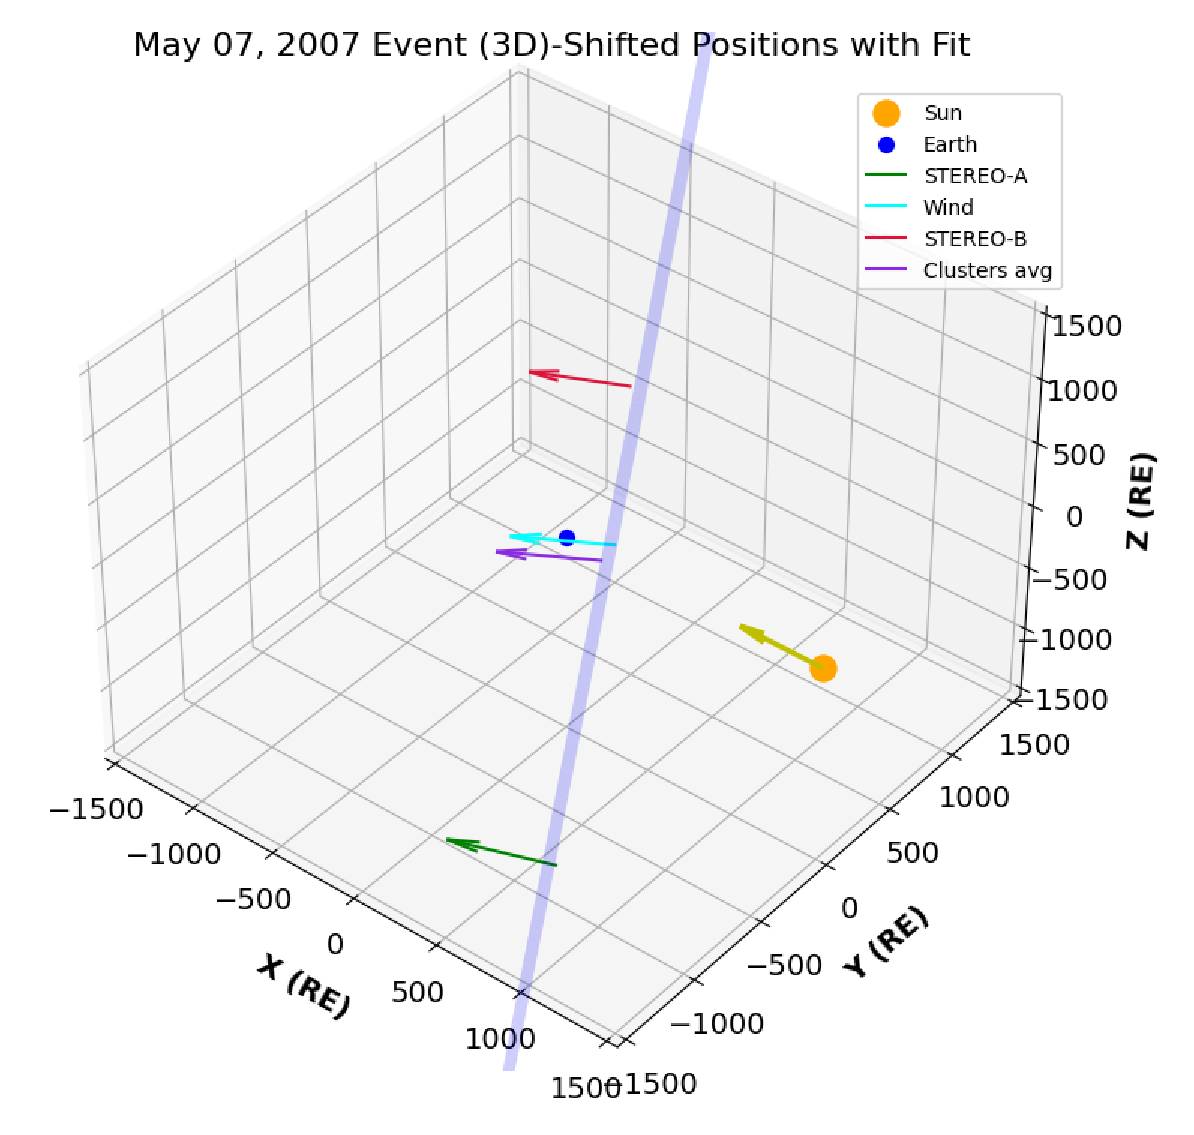
\includegraphics[width=.45\linewidth]{jgr-2023-ipshocks-f17c.eps}
%\caption{A 3D sketch of the propagation of the IP shock through spacecraft-- Wind, STEREO$-$A, and STEREO$-$B, and average position of 4 Cluster satellites. (Top left) Actual shock detected positions. (Top right) The positions of STEREO$-$A, STEREO$-$B, and the average positions of four Cluster spacecraft are shifted back in time to the shock detection time of the Wind spacecraft. (Bottom) The time-shifted positions are fitted with a plane. The arrows indicate the normal vector direction and the planes perpendicular to the normal vectors indicate the shock surface orientations. The sizes of the planes are arbitrary.\label{fig:05073D}}
%\end{figure}

\begin{sidewaysfigure}
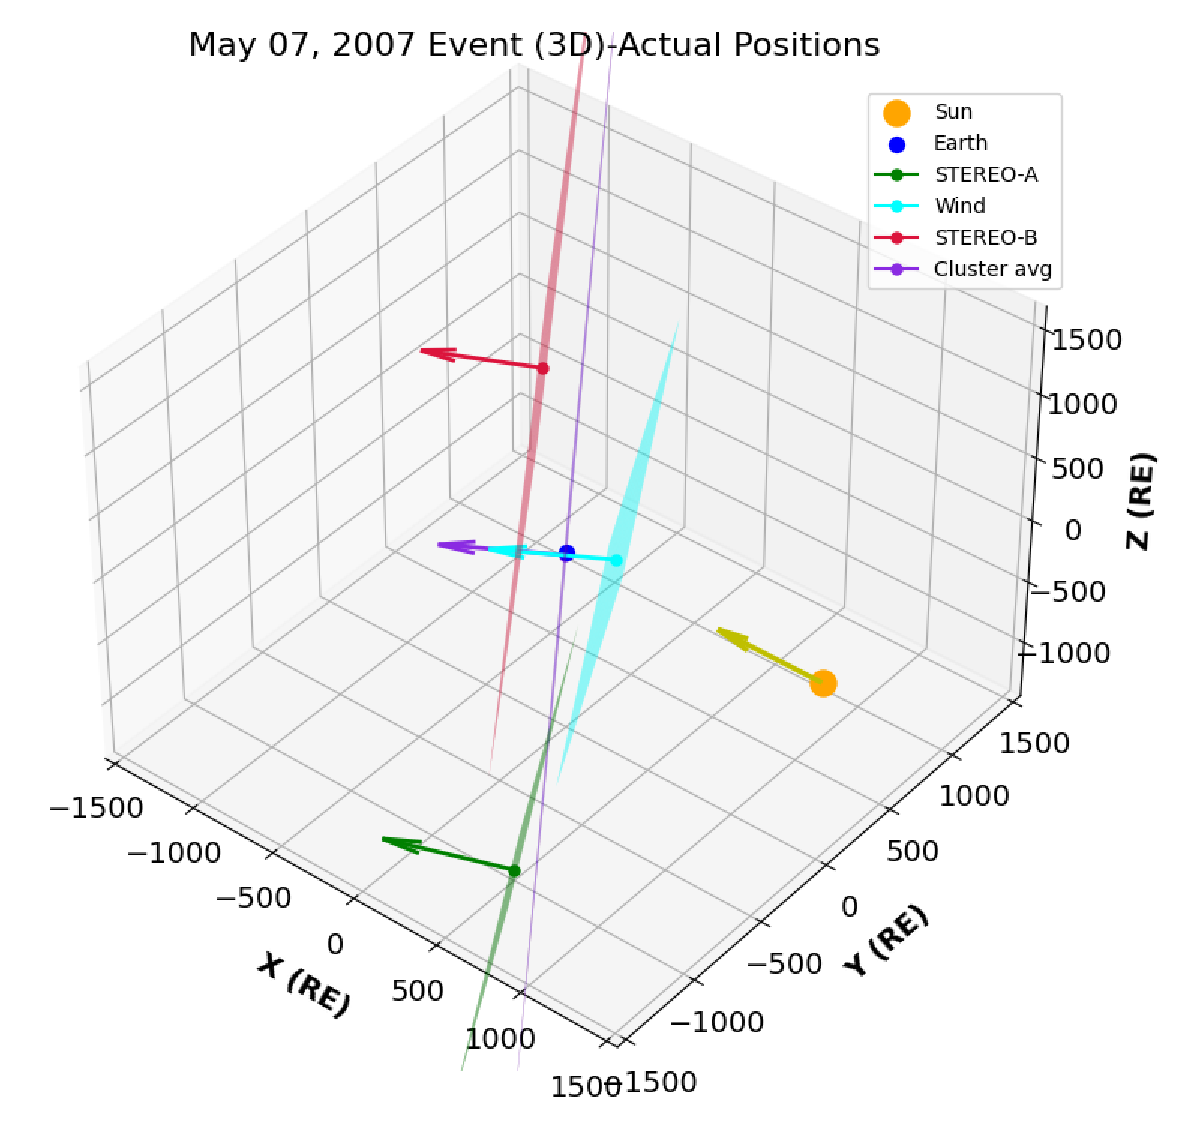
\includegraphics[width=.35\linewidth]{jgr-2023-ipshocks-f17a.eps}
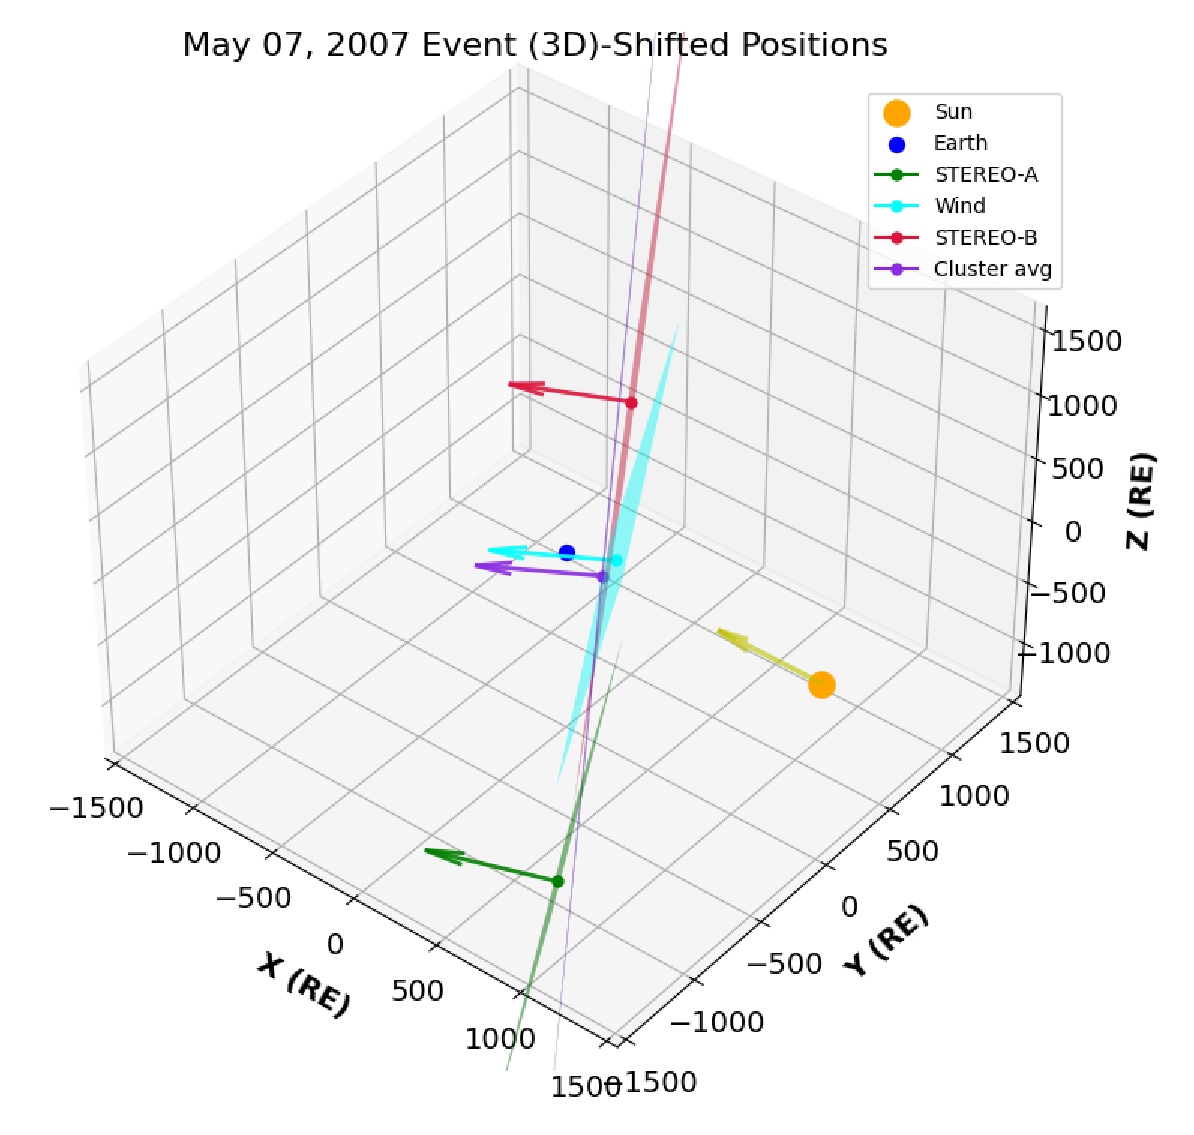
\includegraphics[width=.35\linewidth]{jgr-2023-ipshocks-f17b.eps} 
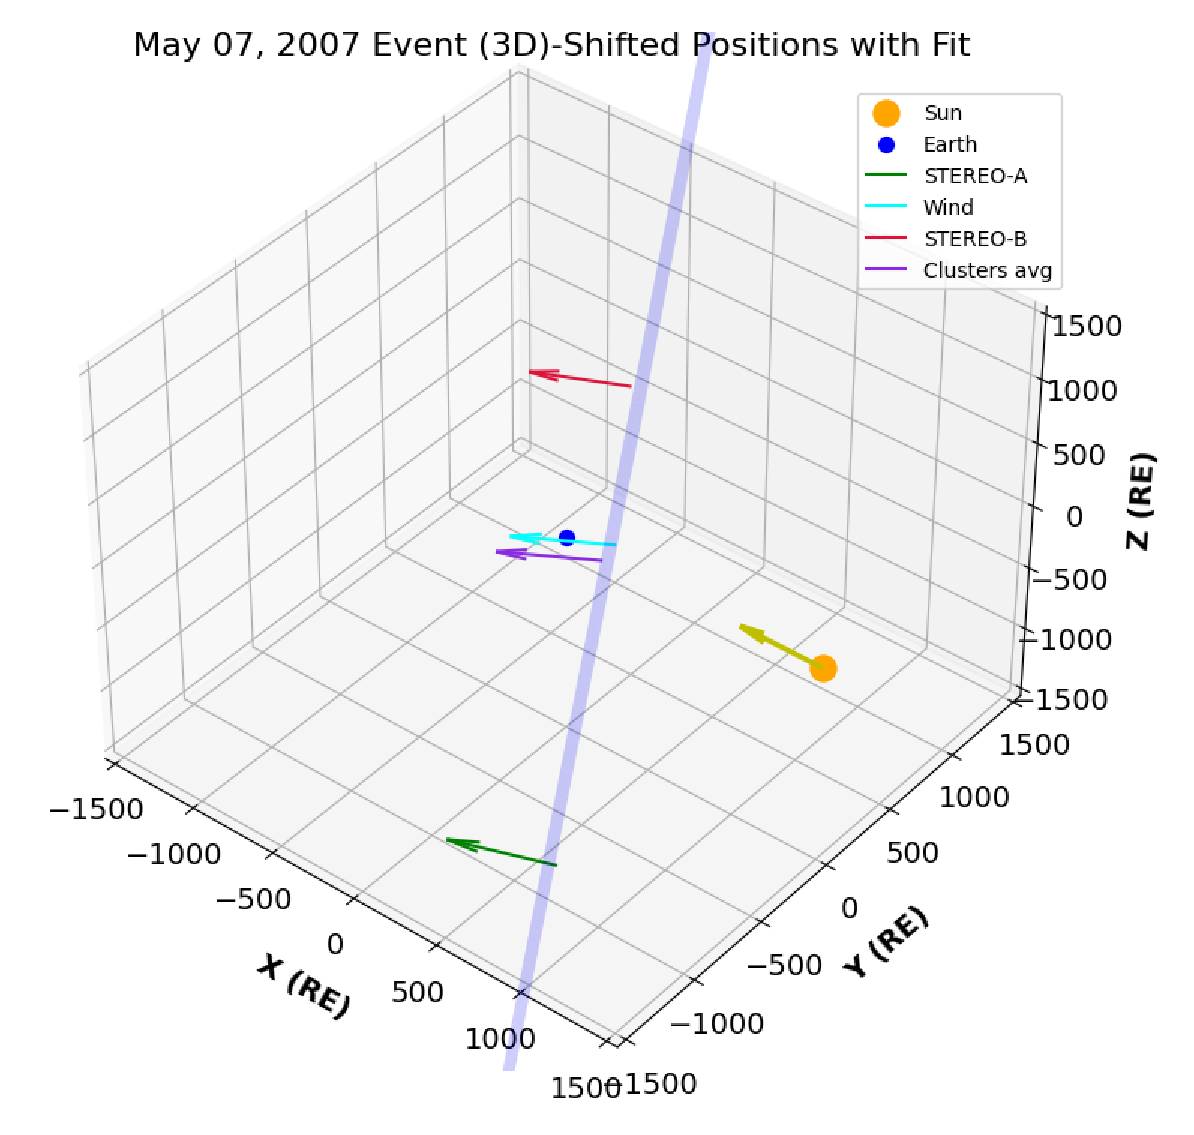
\includegraphics[width=.35\linewidth]{jgr-2023-ipshocks-f17c.eps}
\caption{A 3D sketch of the propagation of the IP shock through spacecraft-- Wind, STEREO$-$A, and STEREO$-$B, and average position of 4 Cluster satellites. (Top left) Actual shock detected positions. (Top right) The positions of STEREO$-$A, STEREO$-$B, and the average positions of four Cluster spacecraft are shifted back in time to the shock detection time of the Wind spacecraft. (Bottom) The time-shifted positions are fitted with a plane. The arrows indicate the normal vector direction and the planes perpendicular to the normal vectors indicate the shock surface orientations. The sizes of the planes are arbitrary.\label{fig:05073D}}
\end{sidewaysfigure}

\pagebreak

 \begin{figure}[!t]
\centering
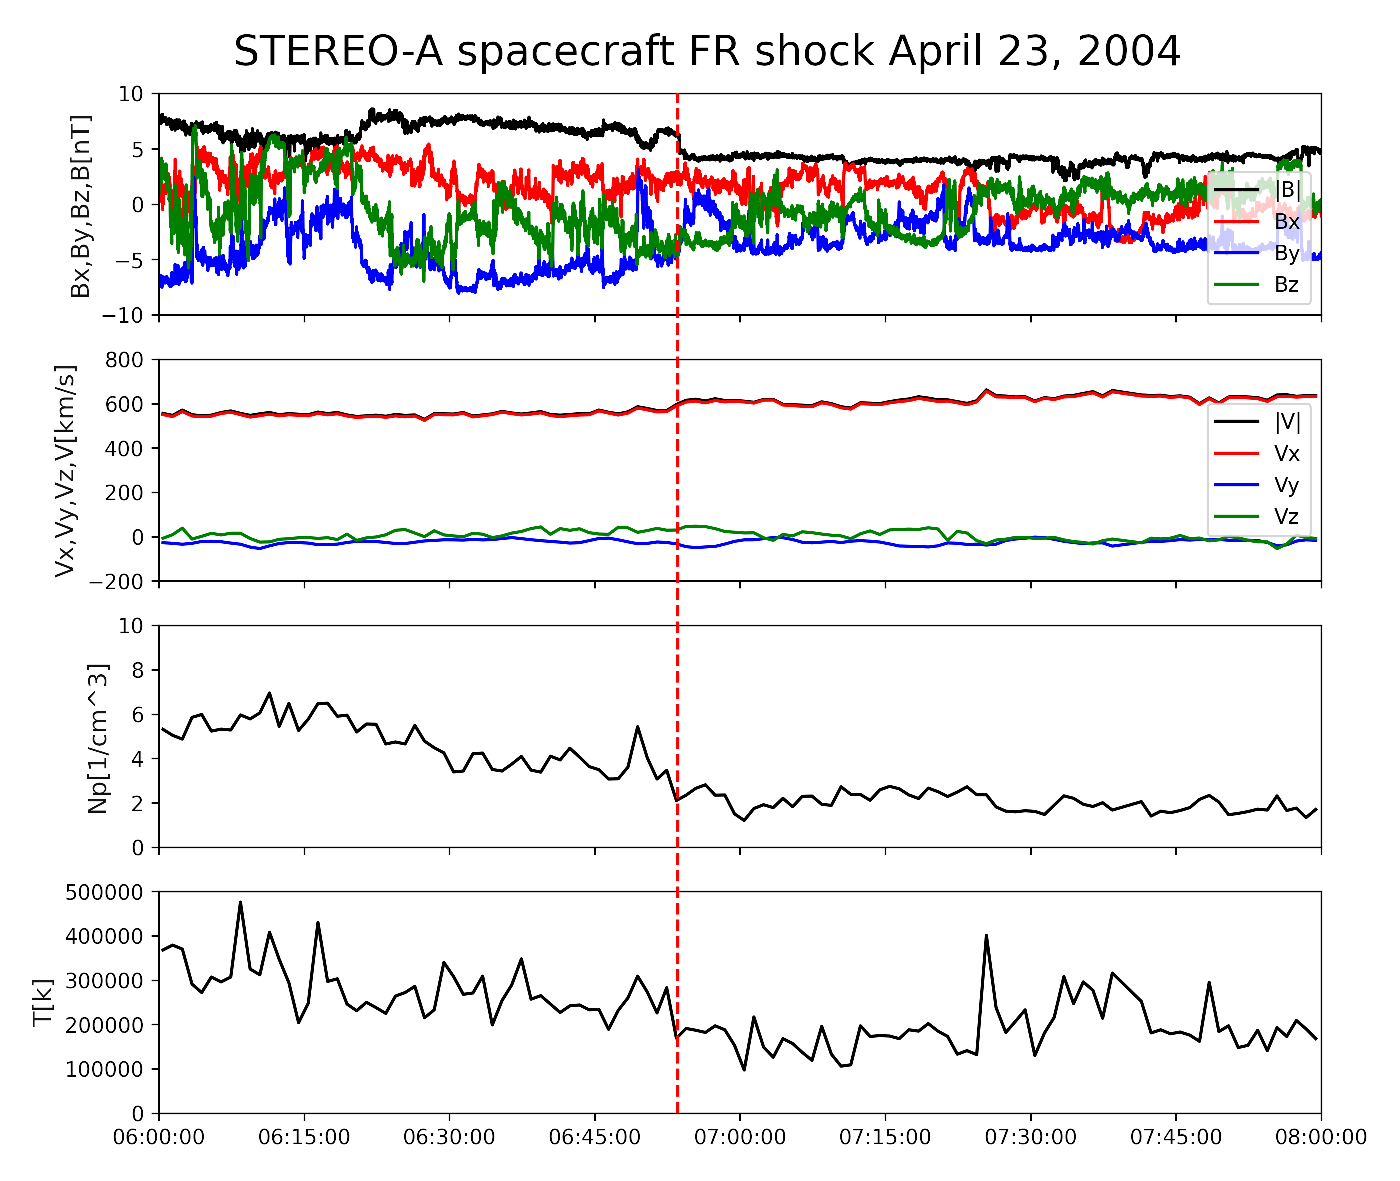
\includegraphics[width=1.0\textwidth]{jgr-2023-ipshocks-f18.eps}
\caption{The plot of the shock detected by the STEREO$-$A spacecraft on April 23, 2007, at 06:53:35 (UTC). FR stands for the fast reverse shock, which means the shock is moving toward its driver. The panels show from top to bottom, the magnetic field magnitude as well as its components, the total velocity and its components, density, and temperature. The dashed red line represents the exact shock time. The duration of the plot is two hours}
\label{fig:staIP0423}
\end{figure}

\pagebreak

\begin{figure}[!t]
\centering
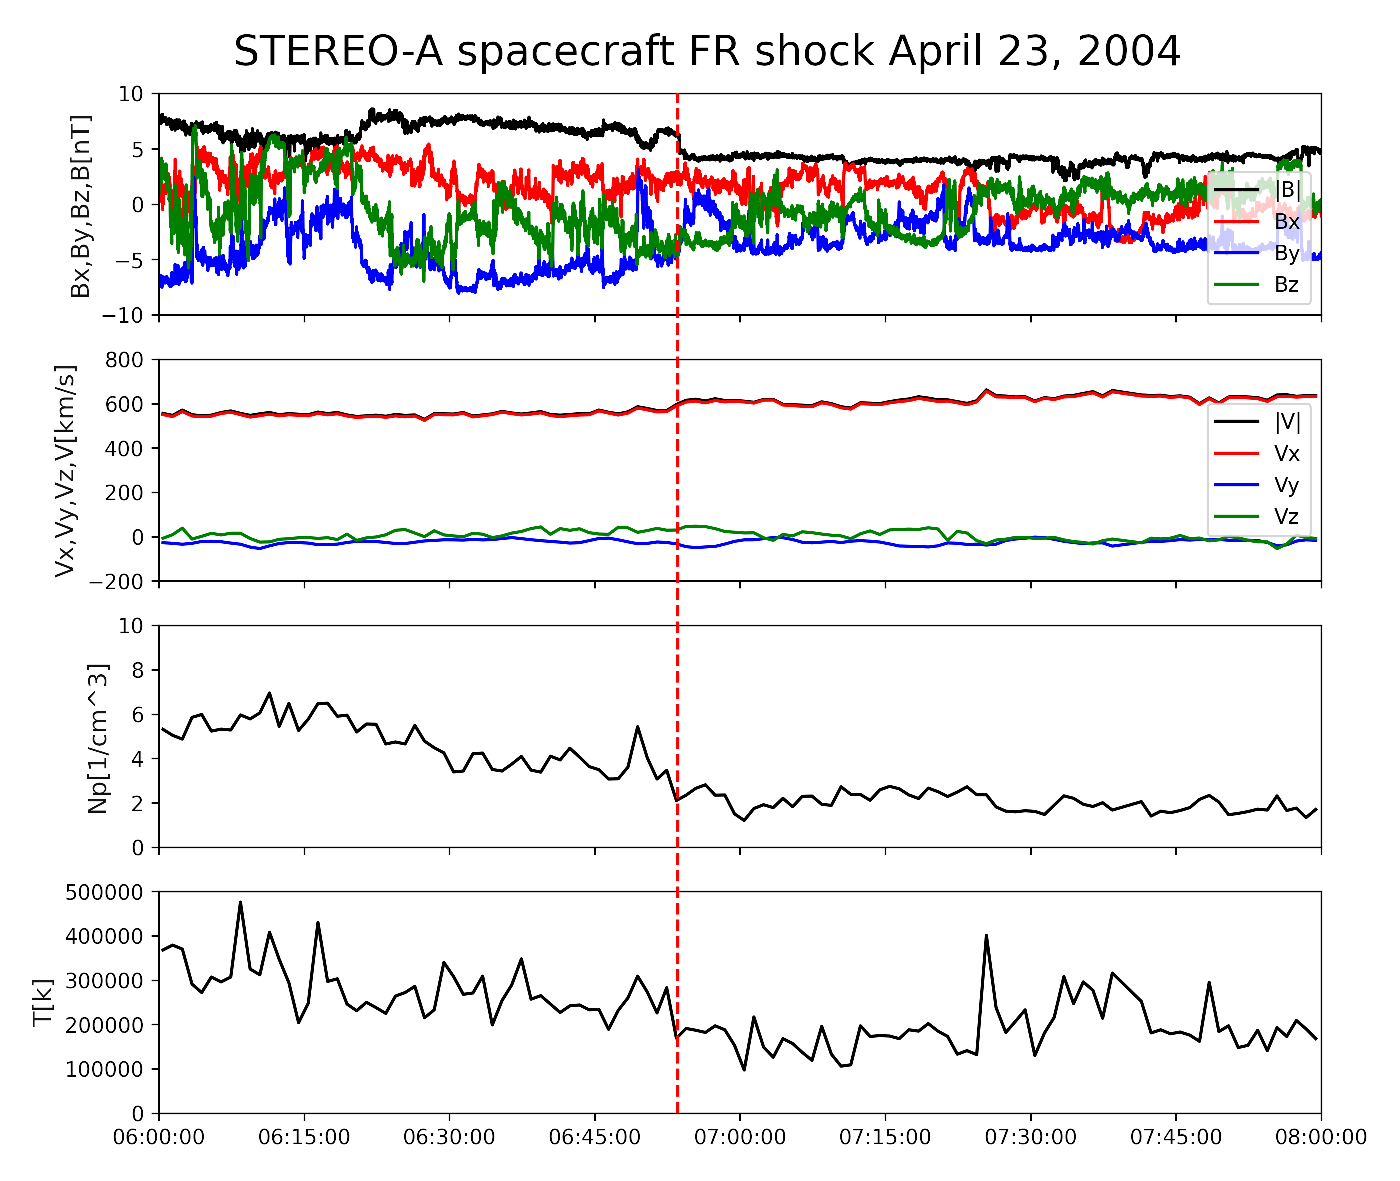
\includegraphics[width=1.\textwidth]{jgr-2023-ipshocks-f19.eps}
\caption{The plot of the shock detected by the ACE spacecraft on April 23, 2007, at 08:57:00 (UTC). The symbols and details of the figures are the same as \ref{fig:staIP0423}. The duration of the plot is two hours.}
\label{fig:aceIP0423}
\end{figure}

\pagebreak

\begin{figure}[!t]
\centering
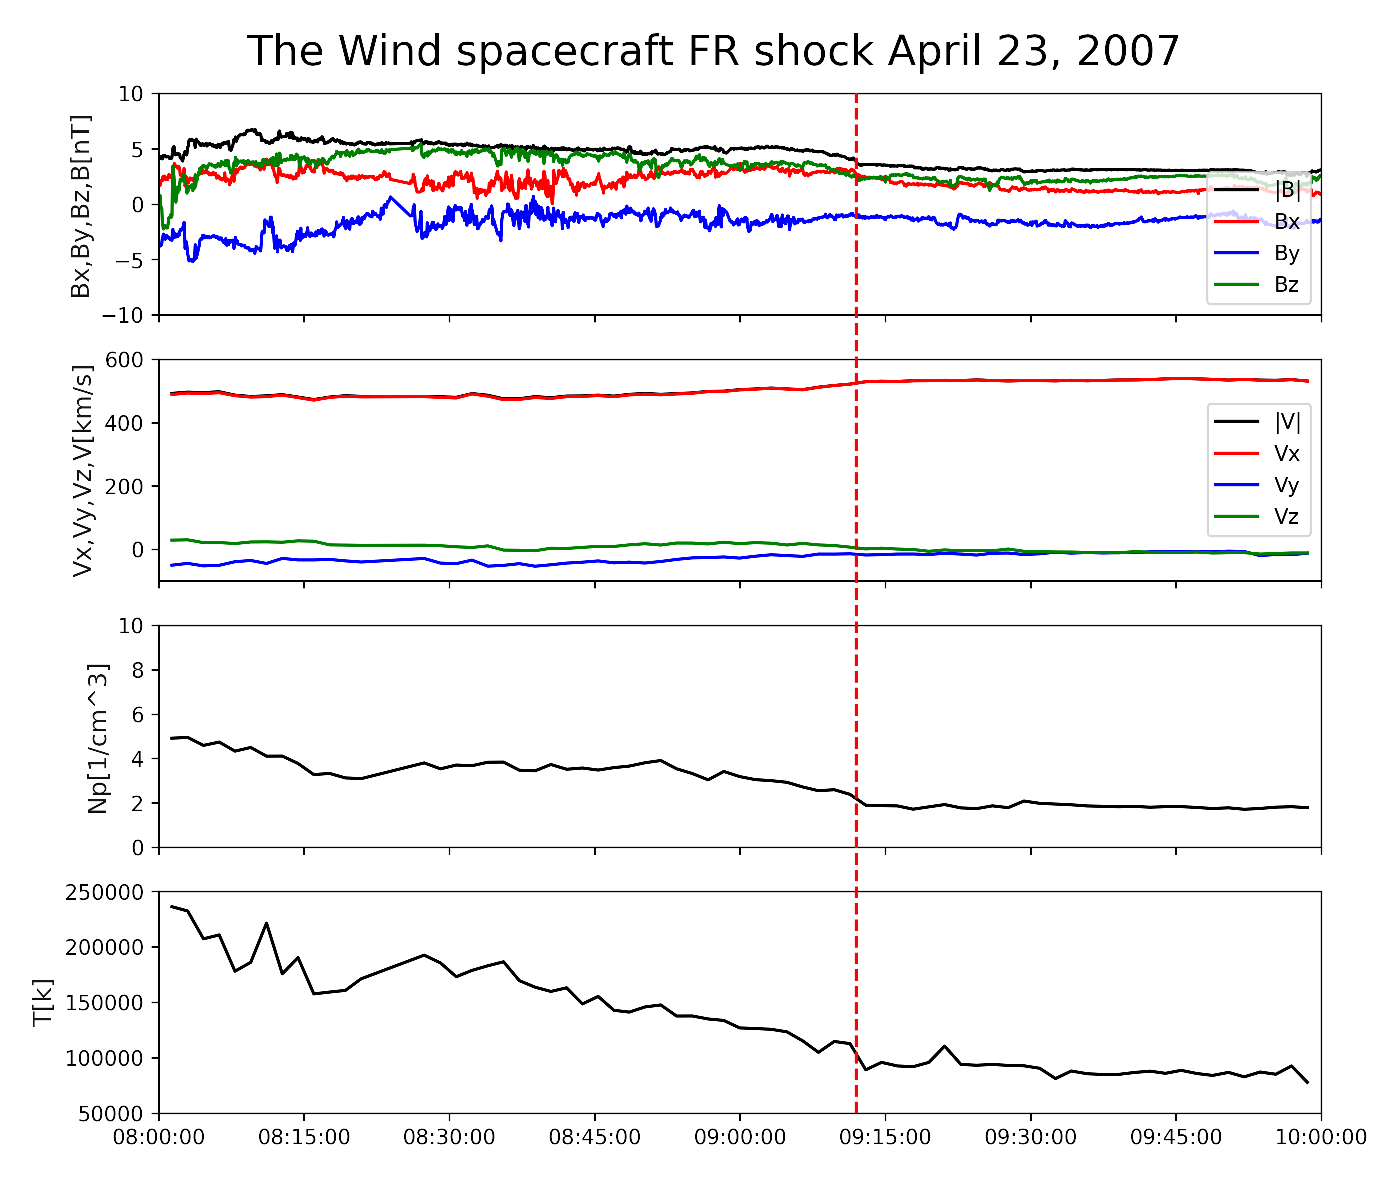
\includegraphics[width=1.\textwidth]{jgr-2023-ipshocks-f20.eps}
\caption{The plot of the shock detected by the Wind spacecraft on April 23, 2007, at 09:12:00 (UTC). The symbols and details of the figures are the same as \ref{fig:staIP0423}. The duration of the plot is two hours.}
\label{fig:WindIP0423}
\end{figure}

\pagebreak

\begin{figure}[!t]
\centering
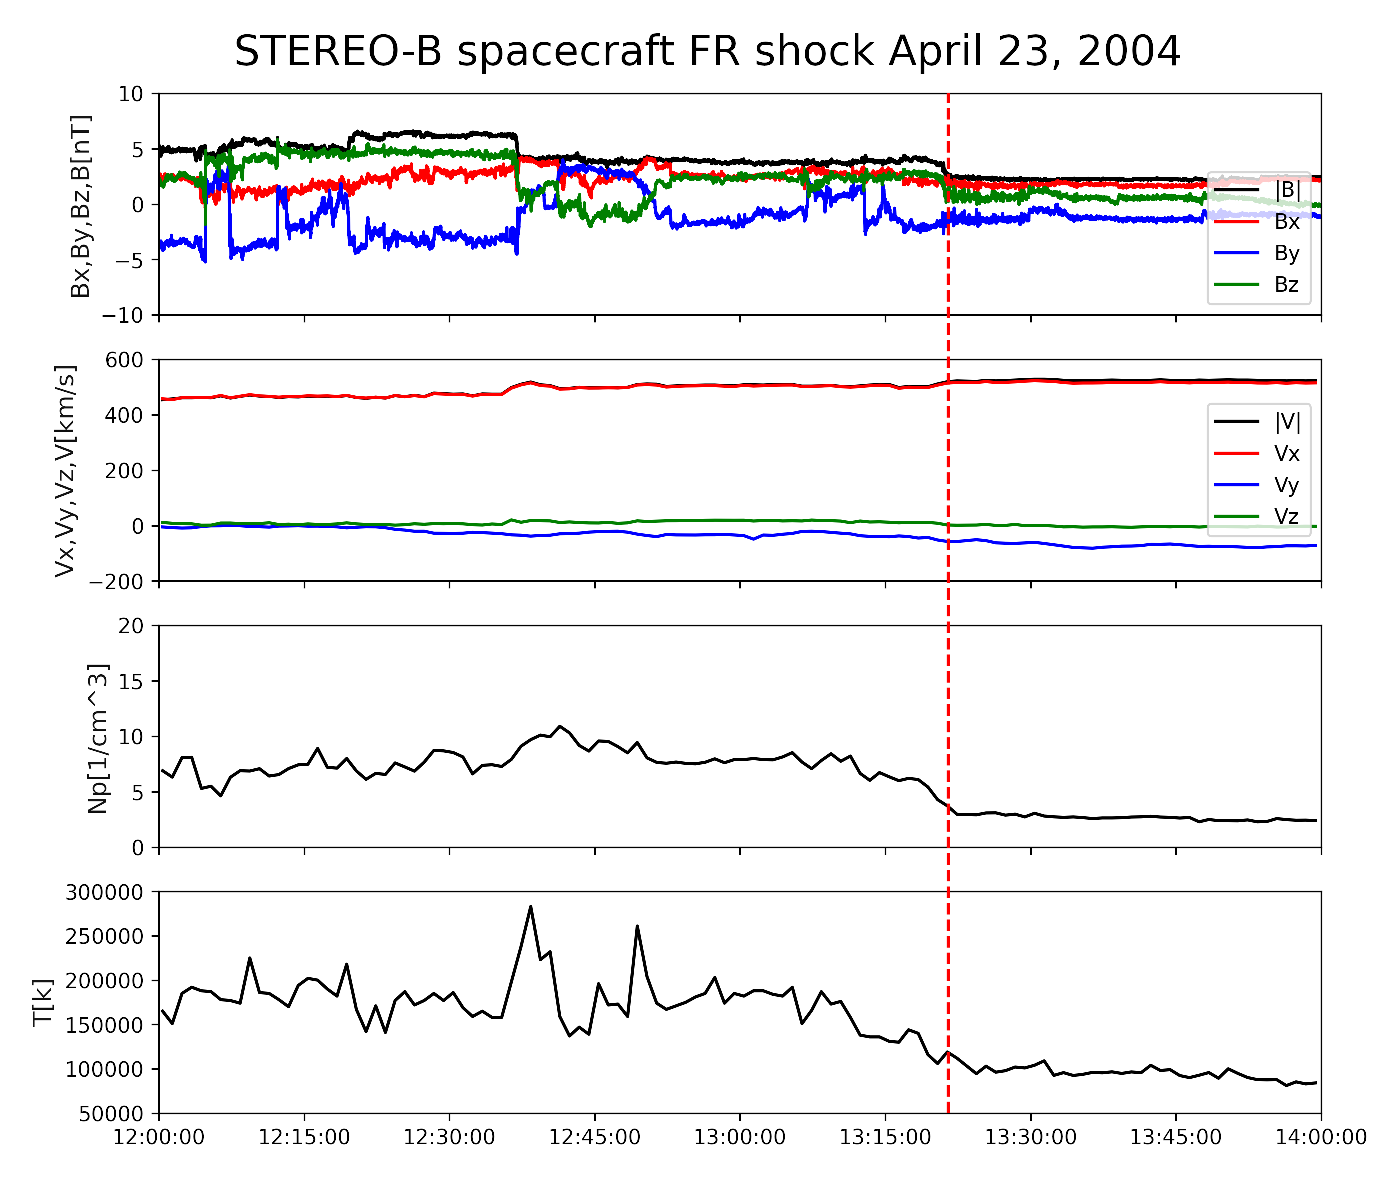
\includegraphics[width=1.\textwidth]{jgr-2023-ipshocks-f21.eps}
\caption{The plot of the shock detected by the Wind spacecraft on April 23, 2007, around 13:21:30 (UTC). The symbols and details of the figures are the same as \ref{fig:staIP0423}. The duration of the plot is two hours.}
\label{fig:stbIP0423}
\end{figure}

 \pagebreak

\begin{figure}[!t]
\centering
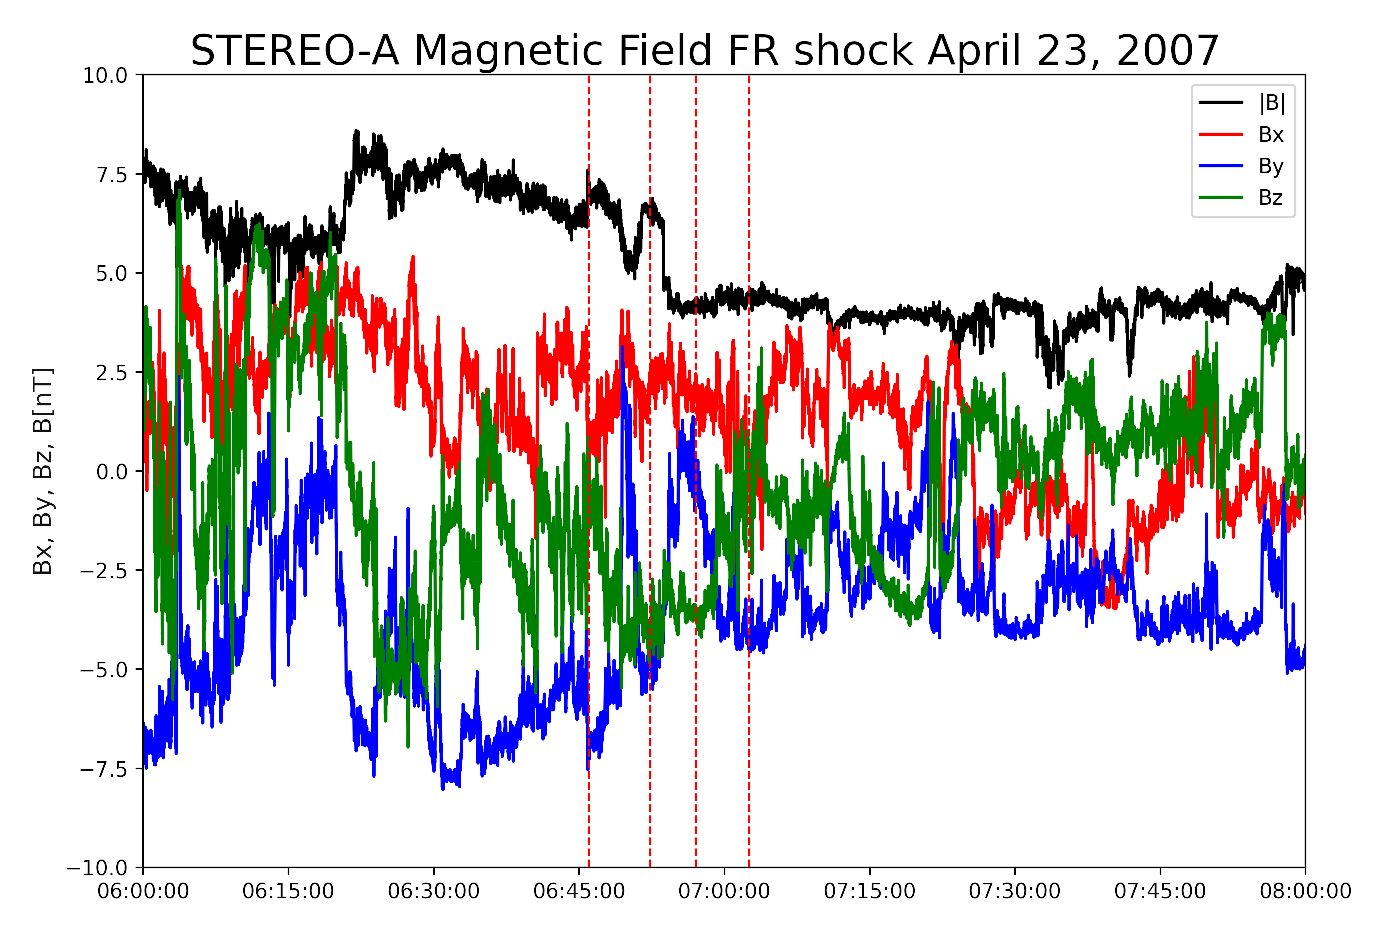
\includegraphics[width=1.\textwidth]{jgr-2023-ipshocks-f22.eps}
\caption{The STEREO$-$A magnetic field measurements. The downstream $\Delta t_{down}$ is between (06:46:00 - 06:52:23), and the upstream $\Delta t_{up}$ is between (06:57:03 - 07:02:34). FR stands for the fast reverse shock, which means the shock is moving toward its driver. The chosen intervals of the upstream and downstream magnetic field. The red dashed lines each represent the downstream starting time and ending time and the upstream starting time and ending time respectively}
\label{fig:staB0423}
\end{figure}

\pagebreak

\begin{figure}[!t]
\centering
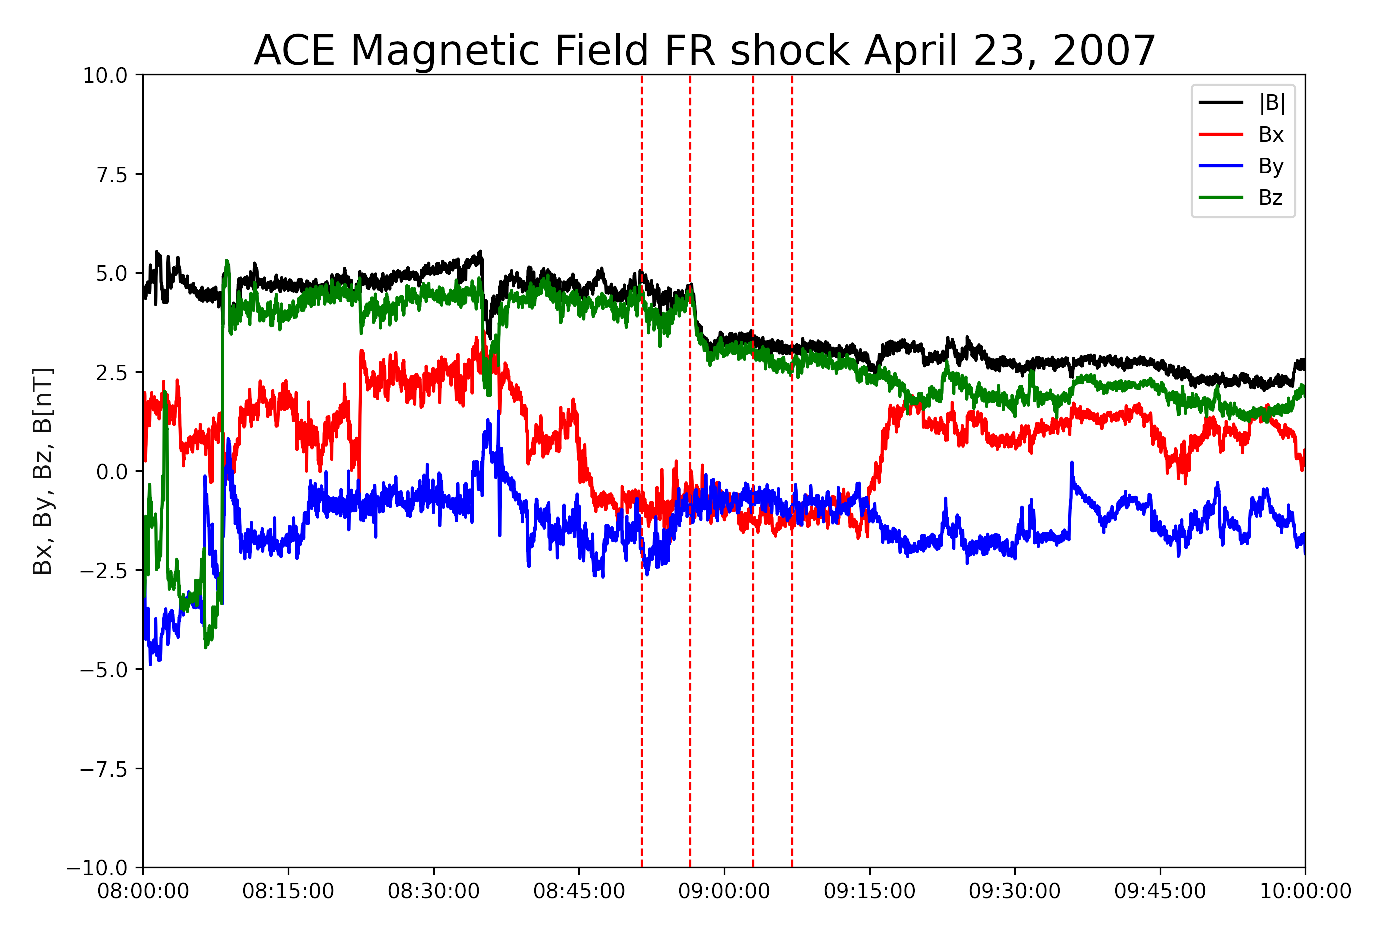
\includegraphics[width=1.\textwidth]{jgr-2023-ipshocks-f23.eps}
\caption{ACE magnetic field measurements. The downstream $\Delta t_{down}$ is between (08:51:30 - 08:56:30), and the upstream $\Delta t_{up}$ is between (09:03:00 - 09:07:00). The symbols and details of the figures are the same as \ref{fig:staB0423}}
\label{fig:aceB0423}
\end{figure}

\pagebreak 

\begin{figure}[!t]
\centering
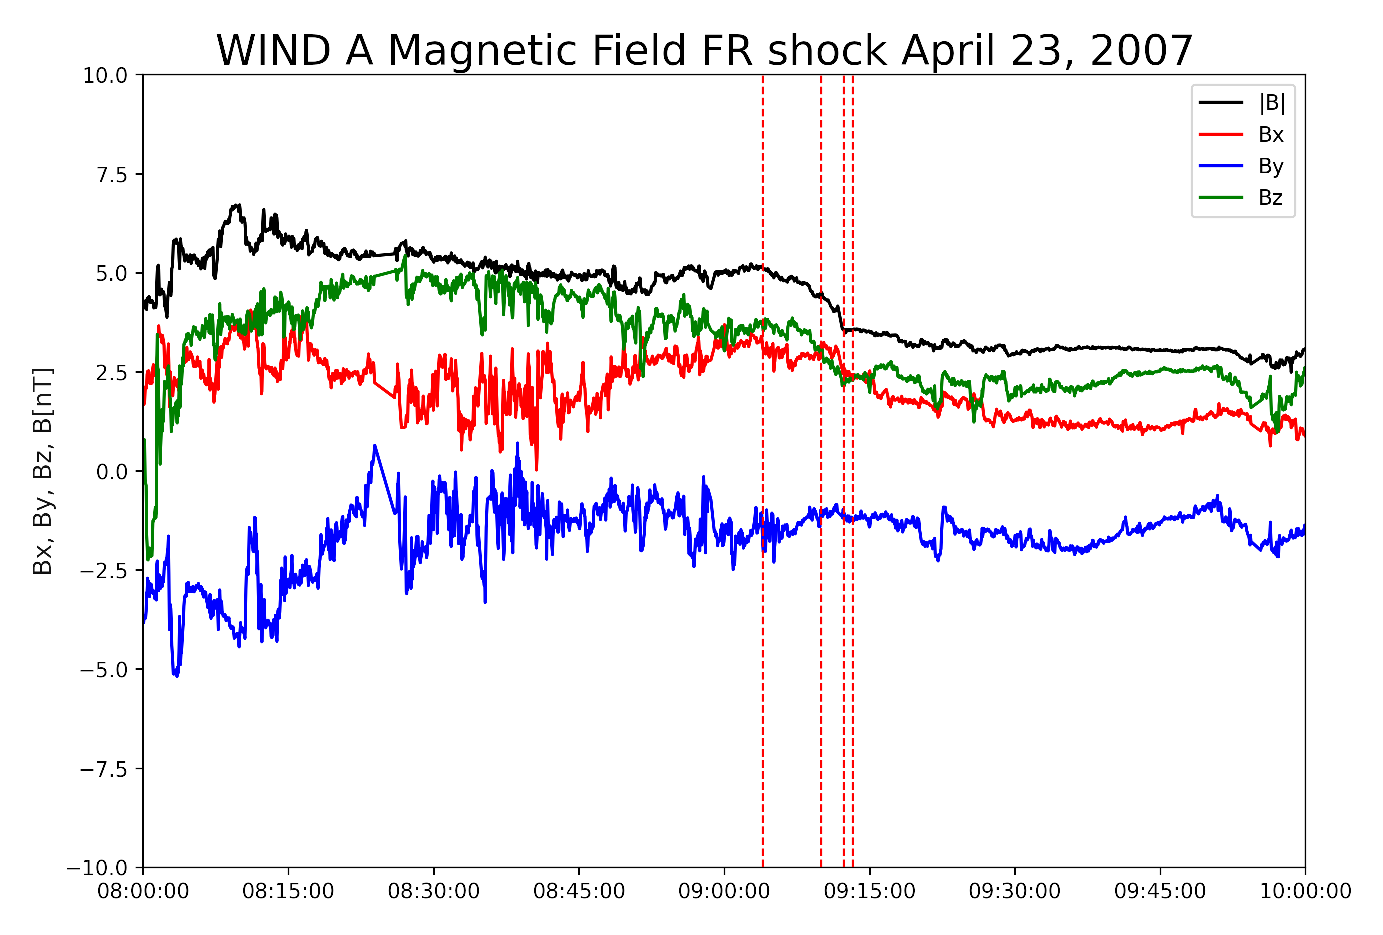
\includegraphics[width=1.\textwidth]{jgr-2023-ipshocks-f24.eps}
\caption{The Wind magnetic field measurements. The downstream $\Delta t_{down}$ is between (09:04:00 - 09:10:00), and the upstream $\Delta t_{up}$ is between (09:12:20 - 09:13:15). The symbols and details of the figures are the same as \ref{fig:staB0423}}
\label{fig:windB0423}
\end{figure}

\pagebreak

\begin{figure}[!t]
\centering
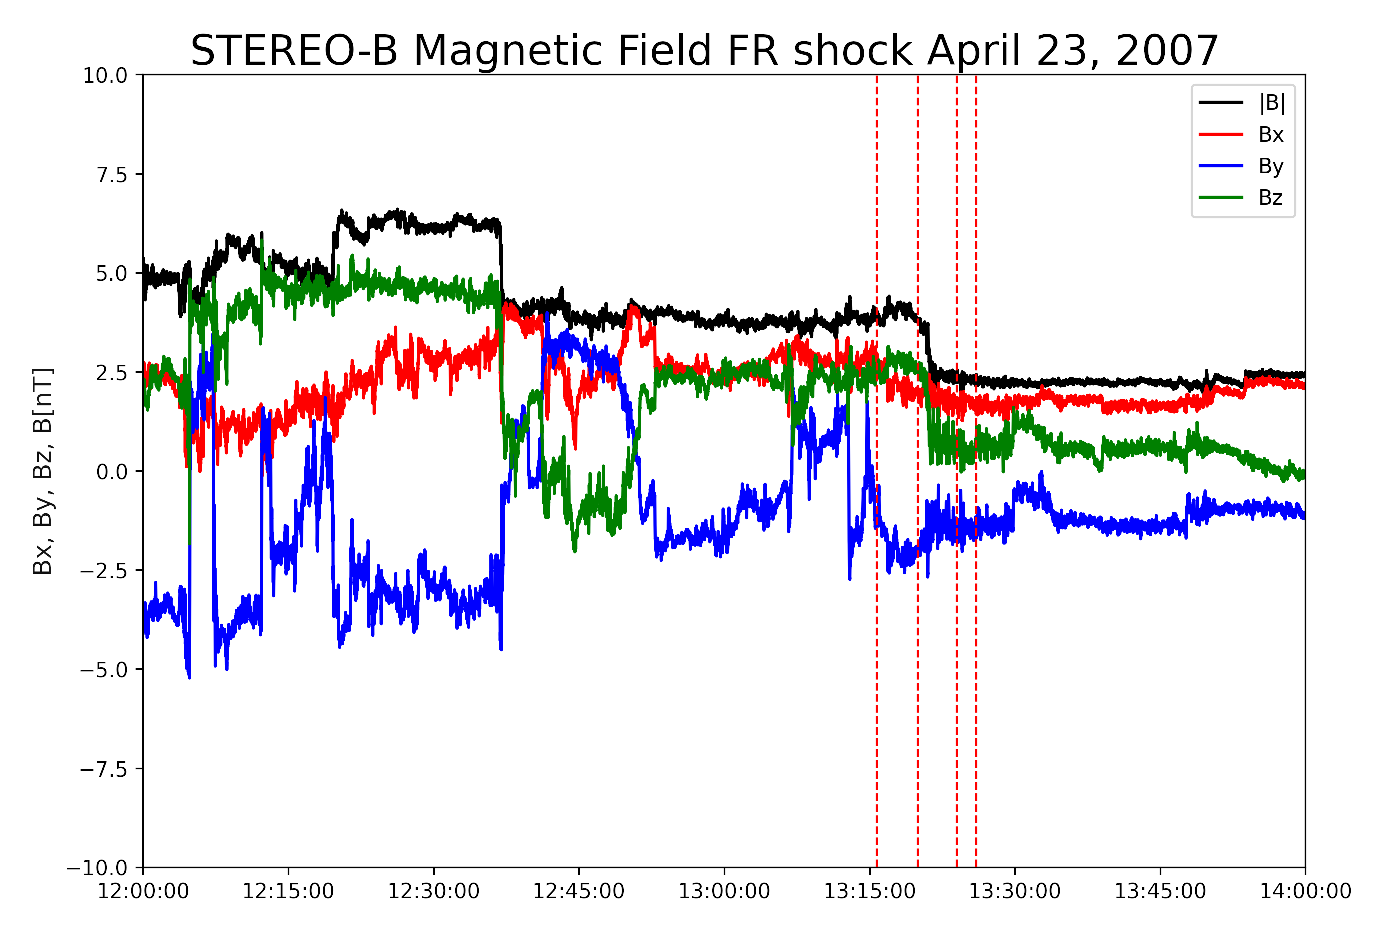
\includegraphics[width=1.\textwidth]{jgr-2023-ipshocks-f25.eps}
\caption{STEREO$-$B magnetic field measurements. The downstream $\Delta t_{down}$ is between (13:15:45 - 13:20:00), and the upstream $\Delta t_{up}$ is between (13:24:00 - 13:26:00). The symbols and details of the figures are the same as on Figure~\ref{fig:staB0423}}
\label{fig:stbB0423}
 \end{figure}

\pagebreak

%\begin{figure}[!t]
%\centering
%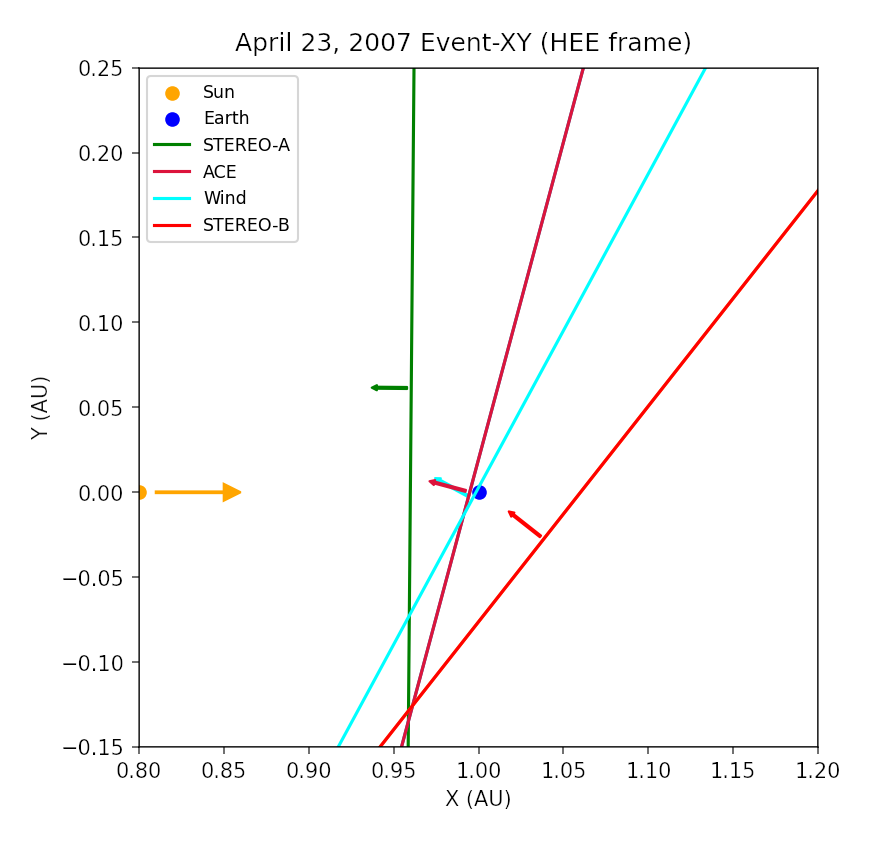
\includegraphics[width=.45\linewidth]{jgr-2023-ipshocks-f26a.eps}
%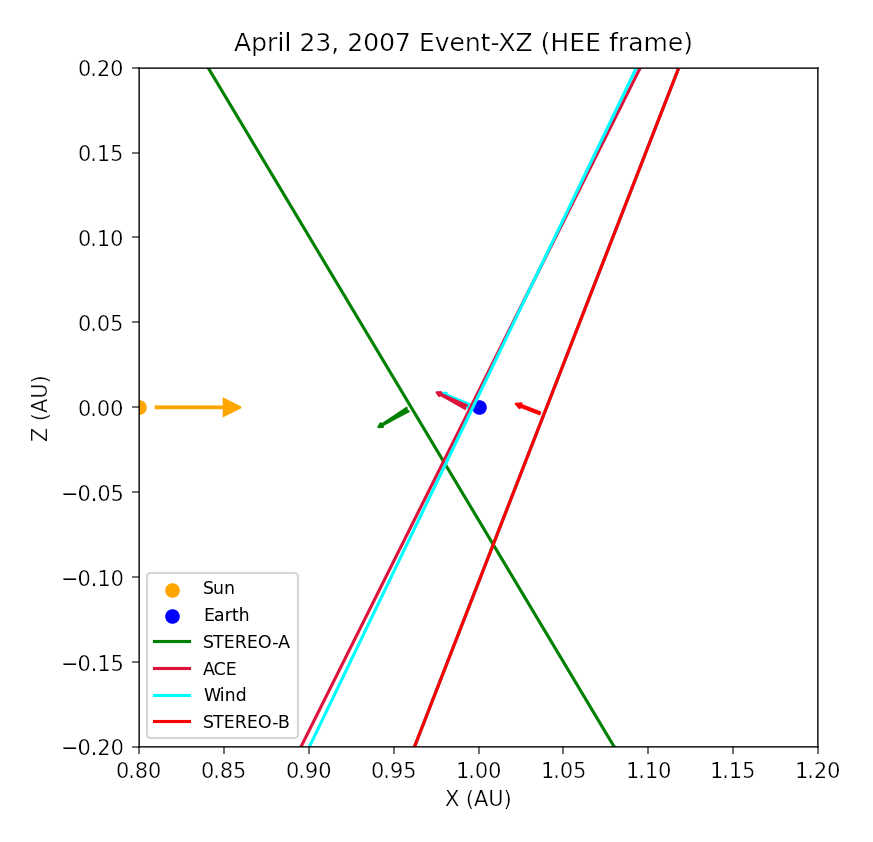
\includegraphics[width=.45\linewidth]{jgr-2023-ipshocks-f26b.eps}
%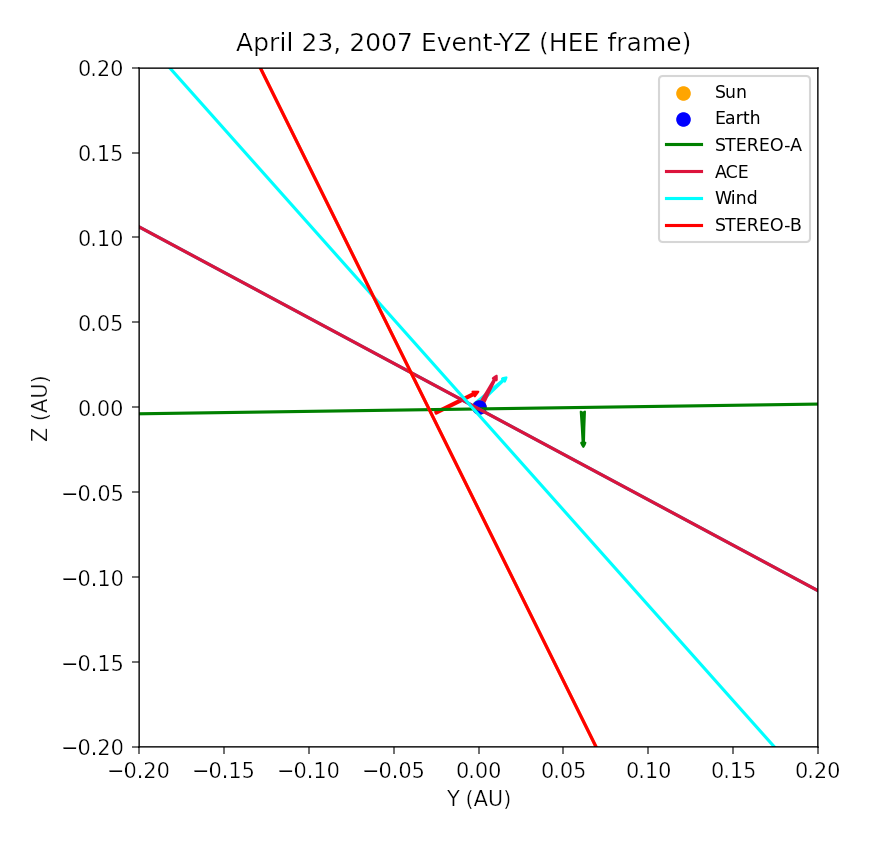
\includegraphics[width=.45\linewidth]{jgr-2023-ipshocks-f26c.eps}
%\caption{2D (Top left) XY, (Top right) XZ, and (Bottom) YZ sketches of the propagation of the IP shock through spacecraft-- STEREO$-$A, ACE, Wind, and STEREO$-$B. The orange arrow represents the Sun-Earth line direction. The arrows on spacecraft positions indicate the normal vector direction calculated from co-planarity method and the lines perpendicular to the normal vectors indicate the shock surface orientations. The sizes of the lines are arbitrary.\label{fig:04232D}}
%\end{figure}

\begin{sidewaysfigure}
\centering
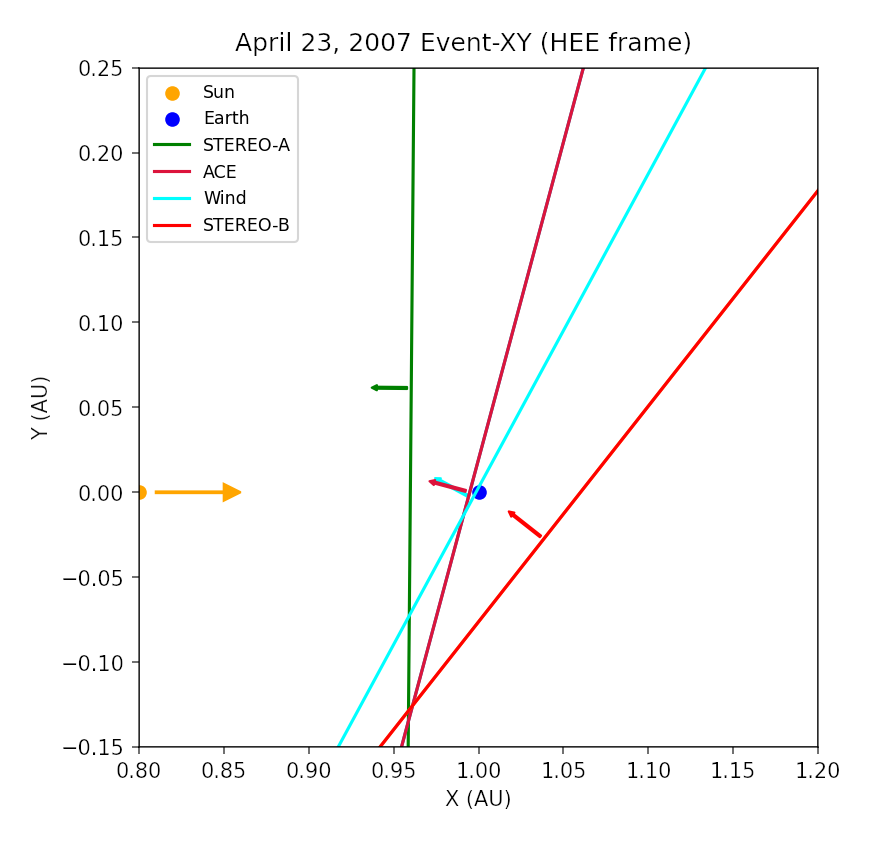
\includegraphics[width=.35\linewidth]{jgr-2023-ipshocks-f26a.eps}
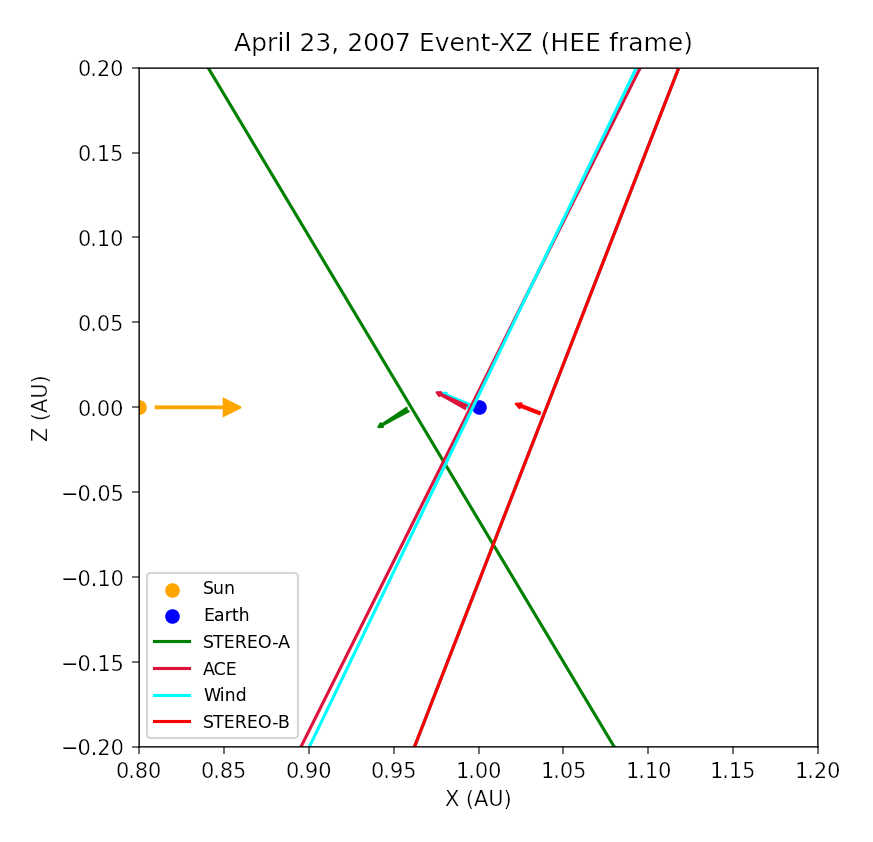
\includegraphics[width=.35\linewidth]{jgr-2023-ipshocks-f26b.eps}
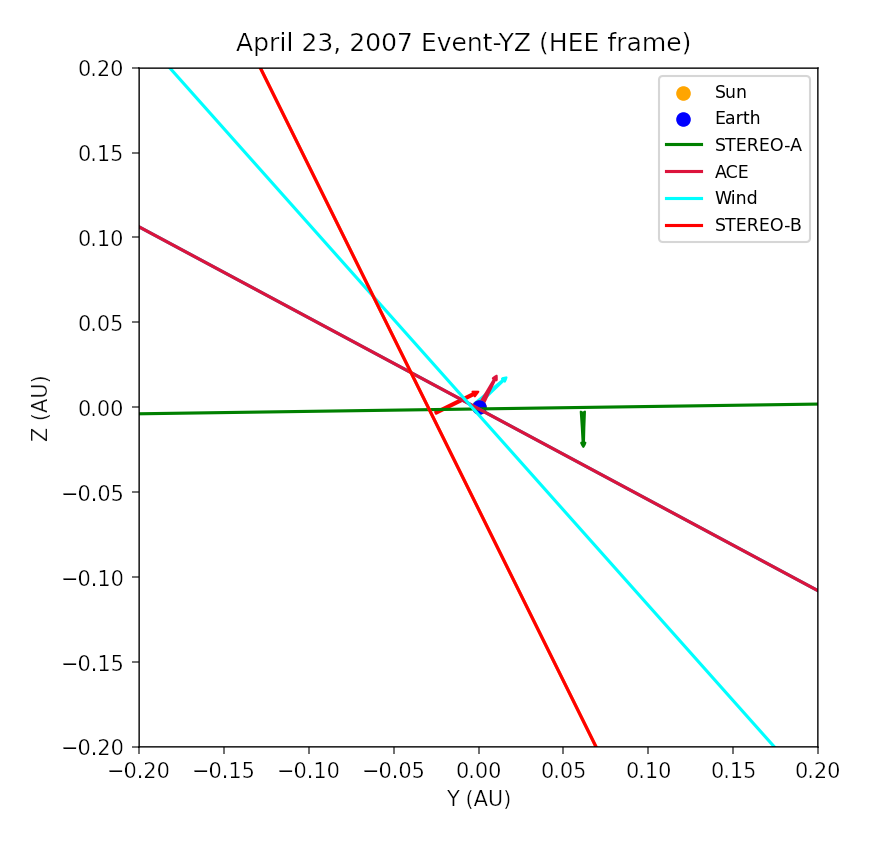
\includegraphics[width=.35\linewidth]{jgr-2023-ipshocks-f26c.eps}
\caption{2D (Top left) XY, (Top right) XZ, and (Bottom) YZ sketches of the propagation of the IP shock through spacecraft-- STEREO$-$A, ACE, Wind, and STEREO$-$B. The orange arrow represents the Sun-Earth line direction. The arrows on spacecraft positions indicate the normal vector direction calculated from co-planarity method and the lines perpendicular to the normal vectors indicate the shock surface orientations. The sizes of the lines are arbitrary.\label{fig:04232D}}
\end{sidewaysfigure}

\pagebreak

%\begin{figure}[!t]
%\centering
%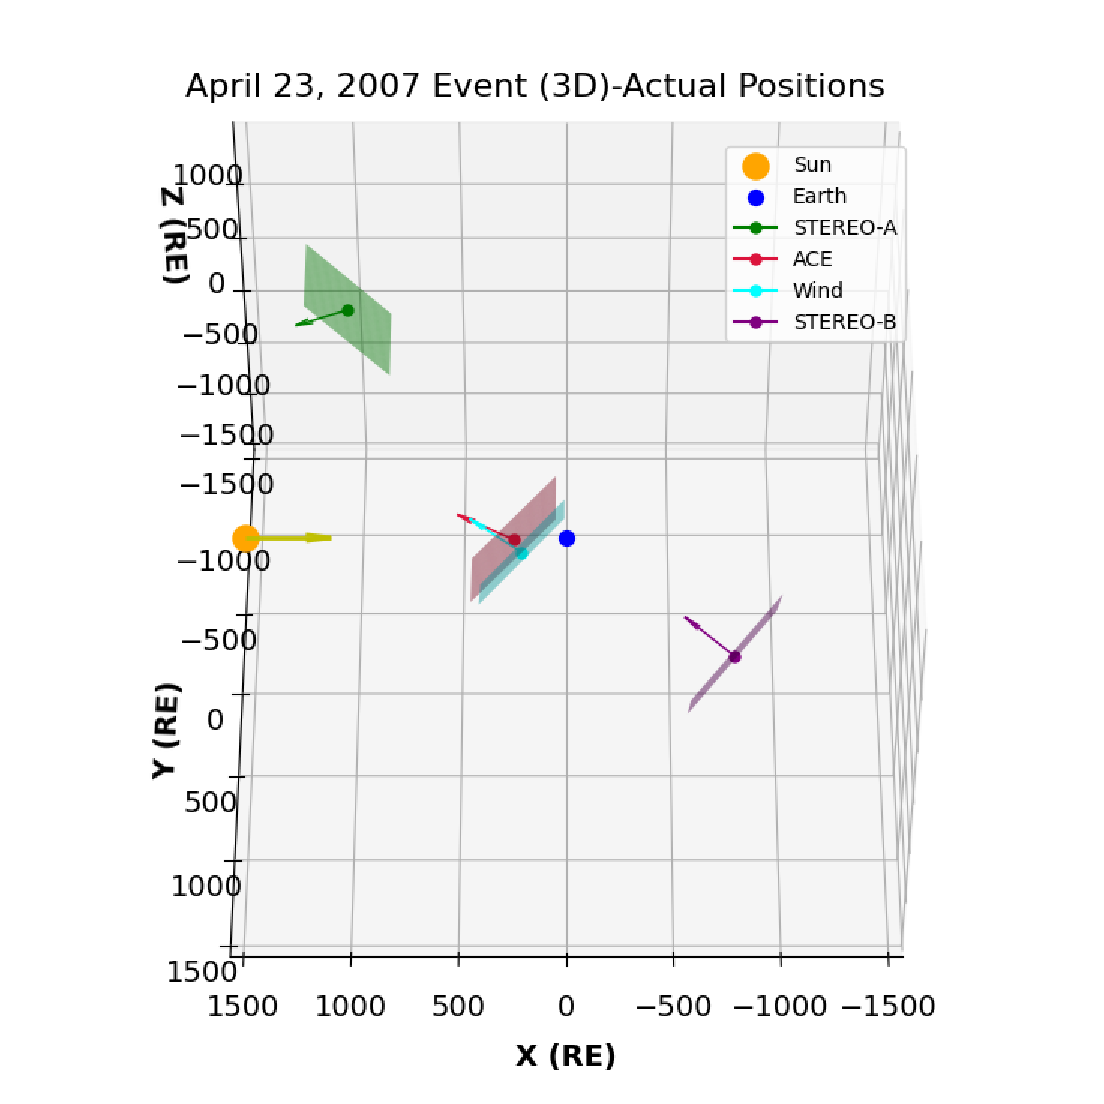
\includegraphics[width=.45\linewidth]{jgr-2023-ipshocks-f27a.eps}
%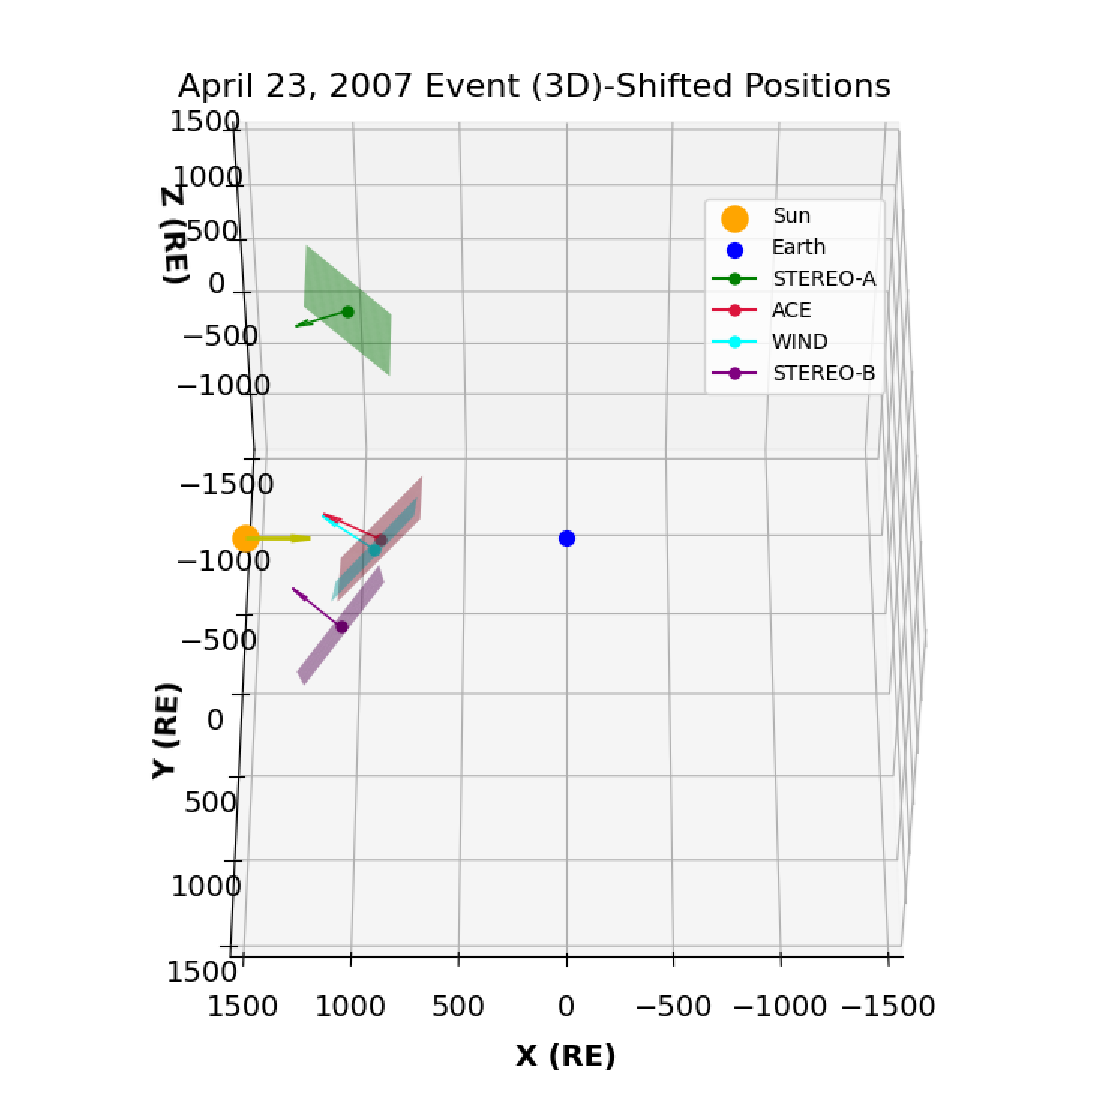
\includegraphics[width=.45\linewidth]{jgr-2023-ipshocks-f27b.eps}
%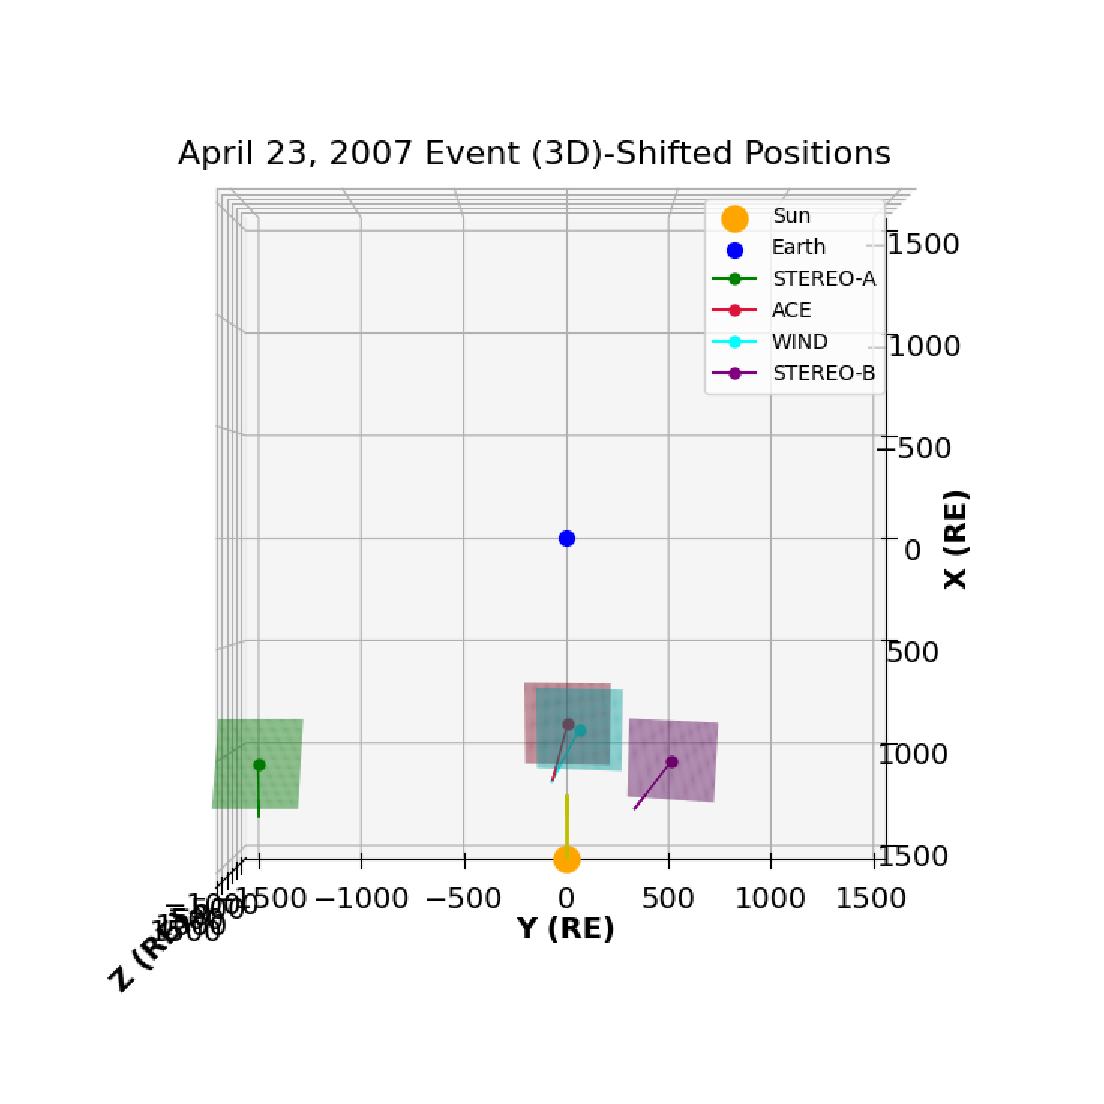
\includegraphics[width=.45\linewidth]{jgr-2023-ipshocks-f27c.eps}
%\caption{ (Top left) A 3D sketch of the propagation of the IP shock through four spacecraft-- STEREO$-$A, Wind, ACE, and STEREO$-$B. (Top right) The positions of Wind, ACE, and STEREO$-$B are shifted back in time to the shock detection time of STEREO$-$A. (Bottom) The shifted positions are shown from the top view. The arrows indicate the normal vector direction and the planes perpendicular to the normal vectors indicate the shock surface orientations. The sizes of the planes are arbitrary.\label{fig:04233D}}
%\end{figure}

\begin{sidewaysfigure}
\centering
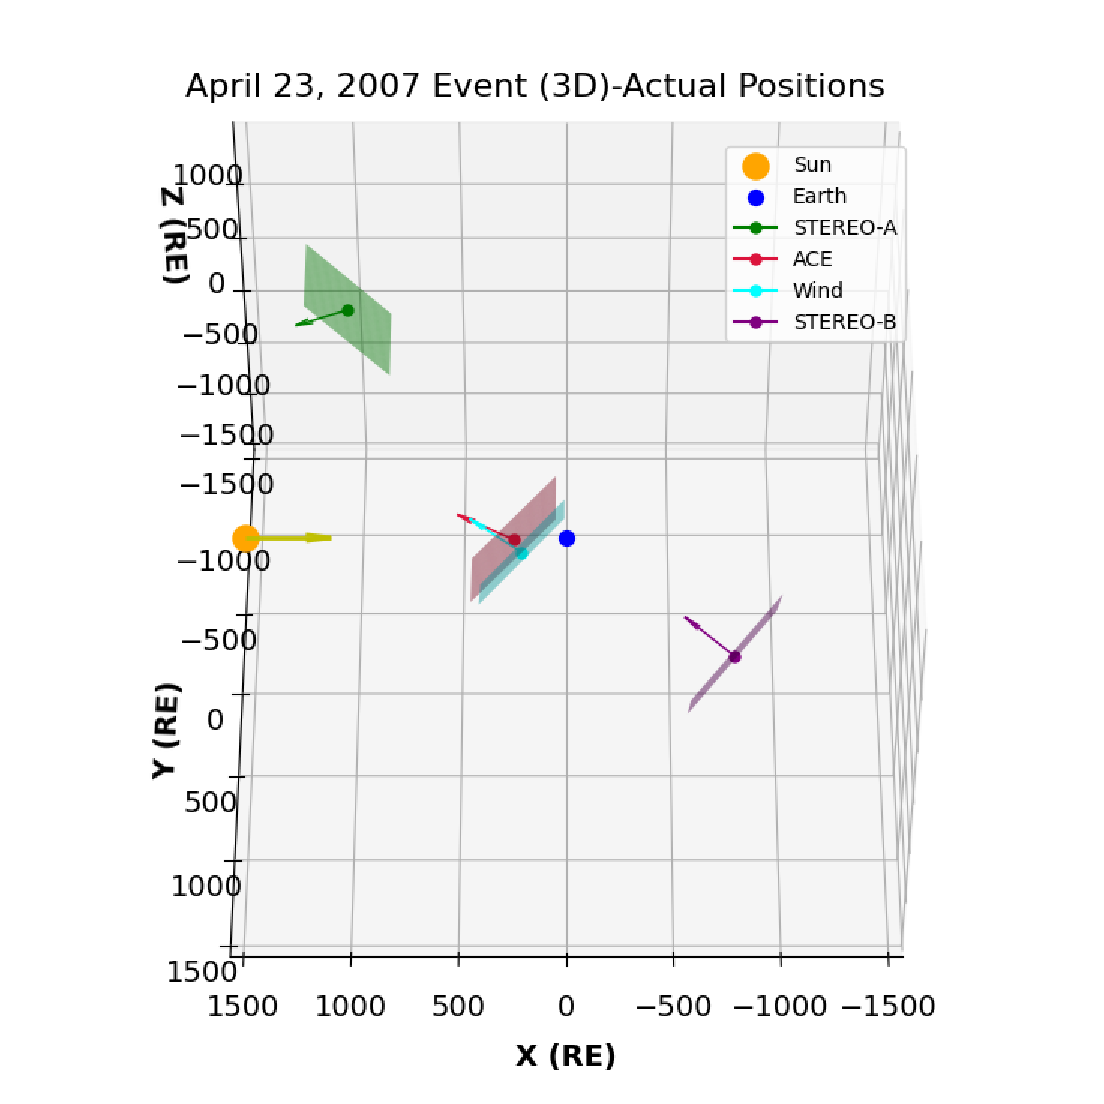
\includegraphics[width=.35\linewidth]{jgr-2023-ipshocks-f27a.eps}
\includegraphics[width=.35\linewidth]{jgr-2023-ipshocks-f27b.eps}
\includegraphics[width=.35\linewidth]{jgr-2023-ipshocks-f27c.eps}
\caption{ (Top left) A 3D sketch of the propagation of the IP shock through four spacecraft-- STEREO$-$A, Wind, ACE, and STEREO$-$B. (Top right) The positions of Wind, ACE, and STEREO$-$B are shifted back in time to the shock detection time of STEREO$-$A. (Bottom) The shifted positions are shown from the top view. The arrows indicate the normal vector direction and the planes perpendicular to the normal vectors indicate the shock surface orientations. The sizes of the planes are arbitrary.\label{fig:04233D}}
\end{sidewaysfigure}

\pagebreak

\begin{figure}[!t]
\centering
\includegraphics[width=1.0\textwidth]{jgr-2023-ipshocks-f28.eps}
\caption{STEREO$-$A PLASTIC bulk velocity, the SWEA electron density, MAG magnetic field magnitude, and the SEPT ion intensity from 110\,keV to 2200\,keV. Periods featuring well-established Co-rotating Interaction Regions (CIRs) from February 1, 2007 to June 1, 2007. It illustrates theeable boosts in ion energy are highlighted with grey shading \cite[Figure~2]{opitz14:_solar_stereo}. \label{fig:cirpaper}}
\end{figure}

\pagebreak

\begin{figure}[!t]
\centering
\includegraphics[width=1.\textwidth]{jgr-2023-ipshocks-f29.eps}
\caption{$K_{p}$-index on May 07, 2007. The green bar indicates moderate geomagnetic activity, while the yellow bar denotes intensifying geomagnetic activity with the red bar being a geomagnetic storm. Here, the red bar indicates a G1-minor geomagnetic storm.}
\label{fig:kp0507}
\end{figure}

\pagebreak

\begin{figure}[!t]
\centering
\includegraphics[width=1.\textwidth]{jgr-2023-ipshocks-f30.eps}
\caption{The $K_{p}$-index on April 23, 2007. The symbols and details of the figure is the same as on Figure~\ref{fig:kp0507}}
\label{fig:kp0423}
\end{figure}

\end{document}

